% Options for packages loaded elsewhere
\PassOptionsToPackage{unicode}{hyperref}
\PassOptionsToPackage{hyphens}{url}
%
\documentclass[
]{book}
\usepackage{lmodern}
\usepackage{amssymb,amsmath}
\usepackage{ifxetex,ifluatex}
\ifnum 0\ifxetex 1\fi\ifluatex 1\fi=0 % if pdftex
  \usepackage[T1]{fontenc}
  \usepackage[utf8]{inputenc}
  \usepackage{textcomp} % provide euro and other symbols
\else % if luatex or xetex
  \usepackage{unicode-math}
  \defaultfontfeatures{Scale=MatchLowercase}
  \defaultfontfeatures[\rmfamily]{Ligatures=TeX,Scale=1}
\fi
% Use upquote if available, for straight quotes in verbatim environments
\IfFileExists{upquote.sty}{\usepackage{upquote}}{}
\IfFileExists{microtype.sty}{% use microtype if available
  \usepackage[]{microtype}
  \UseMicrotypeSet[protrusion]{basicmath} % disable protrusion for tt fonts
}{}
\makeatletter
\@ifundefined{KOMAClassName}{% if non-KOMA class
  \IfFileExists{parskip.sty}{%
    \usepackage{parskip}
  }{% else
    \setlength{\parindent}{0pt}
    \setlength{\parskip}{6pt plus 2pt minus 1pt}}
}{% if KOMA class
  \KOMAoptions{parskip=half}}
\makeatother
\usepackage{xcolor}
\IfFileExists{xurl.sty}{\usepackage{xurl}}{} % add URL line breaks if available
\IfFileExists{bookmark.sty}{\usepackage{bookmark}}{\usepackage{hyperref}}
\hypersetup{
  pdftitle={Environment},
  pdfauthor={Dyrehaugen Web Notebook},
  hidelinks,
  pdfcreator={LaTeX via pandoc}}
\urlstyle{same} % disable monospaced font for URLs
\usepackage{longtable,booktabs}
% Correct order of tables after \paragraph or \subparagraph
\usepackage{etoolbox}
\makeatletter
\patchcmd\longtable{\par}{\if@noskipsec\mbox{}\fi\par}{}{}
\makeatother
% Allow footnotes in longtable head/foot
\IfFileExists{footnotehyper.sty}{\usepackage{footnotehyper}}{\usepackage{footnote}}
\makesavenoteenv{longtable}
\usepackage{graphicx}
\makeatletter
\def\maxwidth{\ifdim\Gin@nat@width>\linewidth\linewidth\else\Gin@nat@width\fi}
\def\maxheight{\ifdim\Gin@nat@height>\textheight\textheight\else\Gin@nat@height\fi}
\makeatother
% Scale images if necessary, so that they will not overflow the page
% margins by default, and it is still possible to overwrite the defaults
% using explicit options in \includegraphics[width, height, ...]{}
\setkeys{Gin}{width=\maxwidth,height=\maxheight,keepaspectratio}
% Set default figure placement to htbp
\makeatletter
\def\fps@figure{htbp}
\makeatother
\setlength{\emergencystretch}{3em} % prevent overfull lines
\providecommand{\tightlist}{%
  \setlength{\itemsep}{0pt}\setlength{\parskip}{0pt}}
\setcounter{secnumdepth}{5}
\usepackage{booktabs}
\usepackage{amsthm}
\makeatletter
\def\thm@space@setup{%
  \thm@preskip=8pt plus 2pt minus 4pt
  \thm@postskip=\thm@preskip
}
\makeatother

\renewcommand\chaptername{}
\usepackage[]{natbib}
\bibliographystyle{apalike}

\title{Environment}
\author{Dyrehaugen Web Notebook}
\date{2022-09-15}

\begin{document}
\maketitle

{
\setcounter{tocdepth}{1}
\tableofcontents
}
\hypertarget{environment}{%
\chapter{Environment}\label{environment}}

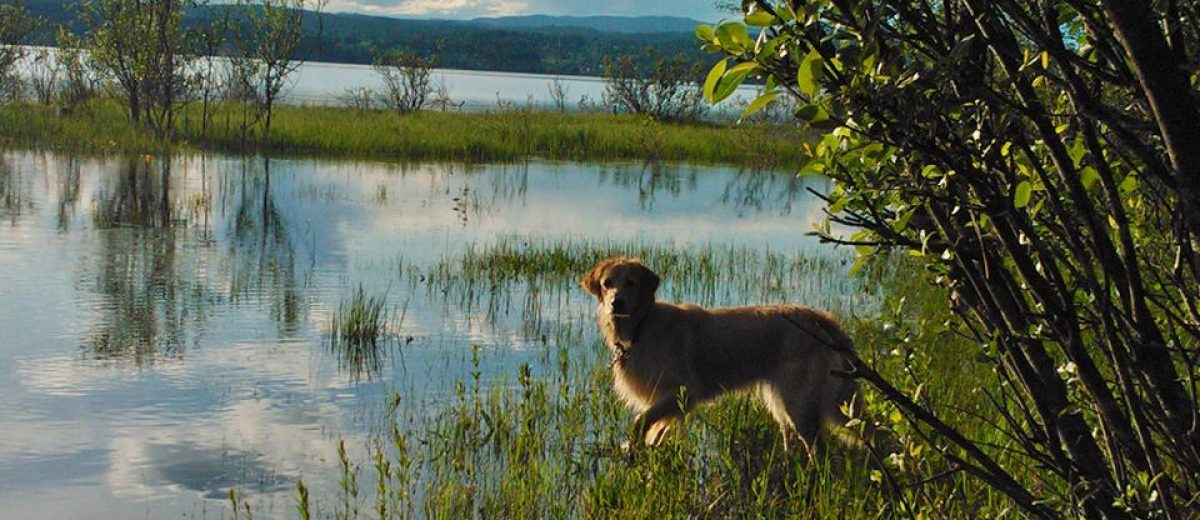
\includegraphics{fig/zelda.jpg}

Here we treat some major environmental issues.
You will not find \emph{Climate Change} here - it has got its own site/book.
The same applies to \emph{Development} i.e.~\emph{Capitalism} as the major
driver of environmental issues.
It too has got its own site/book.

\hypertarget{sustainability}{%
\chapter{Sustainability}\label{sustainability}}

\hypertarget{un-sustainability-goals}{%
\section{UN Sustainability Goals}\label{un-sustainability-goals}}

\emph{Beslik}

The United Nations General Assembly adopted 17 global sustainable development goals (SDGs) in 2015, which may be described as our---humanity's---global strategy for a sustainable world:

1 End all forms of poverty, everywhere.

2 End hunger, achieve food security, improve nutrition, and promote sustainable agriculture.

3 Ensure healthy lives and promote well-being for all.

4 Ensure inclusive and equitable quality education and promote lifelong learning opportunities for all.

5 Achieve gender equality and empower all women and girls.

6 Ensure availability and sustainable management of water and sanitation for all.

7 Ensure access to affordable, reliable, sustainable, and modern energy for all.

8 Promote sustained, inclusive, and sustainable economic growth, full and productive employment, and decent work for all.

9 Build resilient infrastructure, promote inclusive and sustainable industrialization, and foster innovation.

10 Reduce income inequality within and among countries.

11 Make cities and human settlements inclusive, safe, resilient, and sustainable.

12 Ensure sustainable consumption and production patterns.

13 Take urgent action to combat climate change and its impacts by regulating emissions and promoting developments in renewable energy.

14 Conserve and sustainably use the oceans, seas, and marine resources for sustainable development.

15 Protect, restore, and promote sustainable use of terrestrial ecosystems, sustainably manage forests, combat desertification, and halt and reverse land degradation and halt biodiversity loss.

16 Promote peaceful and inclusive societies for sustainable development, provide access to justice for all and build effective, accountable, and inclusive institutions at all levels.

17 Strengthen the means of implementation and revitalize the global partnership for sustainable development.

{[}Beslik (2021) \url{https://esgonasunday.substack.com/p/week-33-where-the-money-tree-grows})

\hypertarget{global-suicide}{%
\section{Global Suicide}\label{global-suicide}}

Humanity is causing a rapid loss of biodiversity and,
with it, Earth's ability to support complex life.

A strange sort of faith lies at the core of mainstream climate advocacy---a largely unexamined belief that the very system that got us into this mess is the one that will get us out of it.

What policy wonks call ``absolute decoupling''---the only kind that would do the climate any good---turns out to be a fantasy akin to a perpetual motion machine, a chimera of growth unhindered by material constraints. One recent analysis of 835 peer-reviewed articles on the subject found that the kind of massive and speedy reductions in emissions that would be necessary to halt global warming ``cannot be achieved through observed decoupling rates.'' The mechanism on which mainstream climate policy is betting the future of the species, and on which the possibility of green growth rests, appears to be a fiction.

\href{https://newrepublic.com/article/161575/climate-change-effects-hurtling-toward-global-suicide}{Ehrenreich (2021) New Republic}

\href{https://www.frontiersin.org/articles/10.3389/fcosc.2020.615419/full}{Bradshaw (2020) Frontiers of Conservation Science}

\hypertarget{resilience}{%
\chapter{Resilience}\label{resilience}}

\hypertarget{de-complexification}{%
\section{De-complexification}\label{de-complexification}}

\emph{King Abstract}

Human civilisation has undergone a continuous trajectory of rising sociopolitical com-
plexity since its inception; a trend which has undergone a dramatic recent acceleration. This phe-
nomenon has resulted in increasingly severe perturbation of the Earth System, manifesting recently
as global-scale effects such as climate change. These effects create an increased risk of a global `de-
complexification' (collapse) event in which complexity could undergo widespread reversal. `Nodes
of persisting complexity' are geographical locations which may experience lesser effects from `de-
complexification' due to having `favourable starting conditions' that may allow the retention of a
degree of complexity. A shortlist of nations (New Zealand, Iceland, the United Kingdom, Australia
and Ireland) were identified and qualitatively analysed in detail to ascertain their potential to form
`nodes of persisting complexity' (New Zealand is identified as having the greatest potential). The
analysis outputs are applied to identify insights for enhancing resilience to `de-complexification'.

\emph{King Memo}

The globe-spanning, energy-intensive industrial civilisation that characterises the
modern era represents an anomalous situation when it is considered against the majority
of human history.

The major shift resulting from the spread of agriculture led to consistent energetic and
material surpluses which, in turn, allowed for the establishment of fixed urban settlements,
hierarchal societies and organisational complexity such as labour specialisation. The
emergence of these phenomena set in motion enhancing feedback mechanisms (e.g., food
surpluses) that led to increasing populations and the spatial expansion of agriculture and
human activity over the majority of the Earth.

The growth of the extent and complexity
of human civilisation continued for centuries but was ultimately constrained by reliance
on natural flows of energy (primarily insolation captured through photosynthesis and
the availability of biomass in which it was stored) and the application of human/animal
muscle power to utilise energy and material resources. Overcoming this limit commenced
from approximately 1800 (the start of the Industrial Revolution) through the large-scale
exploitation of the very large energy stock contained within fossil carbon deposits using
newly developed technologies.

The global population and industrial capacity
grew rapidly for approximately 150 years but achieved near-exponential growth only
from approximately the middle of the 20th century. This period, characterised as the
`Great Acceleration', has generated the most rapid and profound of all the changes
described above, resulting from the strengthening of the feedbacks initiated at the start of
the Industrial Revolution.

The `Great Acceleration' is characterised by substantial and ongoing increases in
societal complexity and the extent and intensity of human activities across a broad spectrum
of measures.
The aggregate effect of this dramatic growth
has been the strong and increasing perturbation of the Earth system and the biosphere,
making collective human civilisation a major force acting at global scale.

From a biophysical perspective, human civilisation is a non-equilibrium thermodynamic
or dissipative system that must maintain a minimum level of available exergy
to avoid entropic decay and a yet higher level to permit physical growth. From the
ecological economics perspective, it can be viewed as an `economic superorganism' that
seeks to maximise energy consumption through self-organisation at a large scale, or the
`megamachine' driven to ever greater size and scope by the enhancing feedbacks of capital
accumulation.

The Earth System is, however, finite in spatial extent, energetic capacity and overall
complexity, and the ongoing expansion of human endeavours has and will continue to
result in the Earth System's limits being exceeded and the system being moved out of
equilibrium. The Earth System (characterised as `Gaia') is a self-regulating mechanism {[}6{]},
and observable shifts in the behaviour of Earth Systems may be manifestations of balancing
feedbacks resulting from the strong and growing perturbation from human activities. These
may have the potential to fundamentally undermine the agriculture-based civilisation that
has flourished in benign Holocene conditions.

Four major categories of threats to the ongoing
viability of the high-intensity civilisation has emerged from the `Great Acceleration'.
These phenomena are

\begin{itemize}
\tightlist
\item
  encountering of limits;
\item
  diminishment of returns;
\item
  ecological destruction;
\item
  `risk multipliers'.
\end{itemize}

The peak use rates across multiple crucial resource types shows that
numerous resources had a synchrony of peak use centred on the year 2006. The
phenomenon has implications in terms of the capacity of global society to adapt to physical
scarcity given that limits on the availability of multiple resources may have to be managed
simultaneously, and this may constrain the capacity for substitution and `de-coupling' of
resource use

The availability of high EROI energy
sources (that provide an `excess' of energy) can be linked with socioeconomic complexity
and `higher' societal functions (e.g., education, health care, culture) that are indicative of
higher living standards. `Traditional' fossil fuels have provided a high EROI value for many
decades, but the decline in the quality and accessibility (and therefore EROI) of these fuels,
in parallel with the generally lower net energy provided by other energy sources, could
result in a reduction in global economic output and quality of life.
A transition to an energy system with a high
proportion of renewables may lead to an `energy trap'.

Application of predator--prey population dynamics models to assess
the evolution of four factors (`elites/commoners/nature/wealth'),
identifies that (economic) `elites' preying on resources and the labour of `commoners' can
lead to economic stratification and ecological strain and, ultimately, irreversible societal
collapse.

Sociopolitical complexity has been fundamental to the functioning and success of human
societies post the Agricultural Revolution {[}28{]} and is described as the collective problem-
solving and efficiency-seeking strategies deployed by all organised human societies in re-
sponse to encountering problems, constraints (e.g., energy or water) or aspirations. It may
include: `bureaucracy' in the form of governments; specialisation of roles, occupations and
industries; new technologies; and increased mobility and trade. The sociopolitical com-
plexity (hereafter complexity) provides marginal gains (i.e., net benefits) when initially
deployed, but as further complexity is added, the marginal gains diminish in an inversely
proportional manner. The subsequent progression through zero and then negative marginal
benefit is posited as the factor consistent with societal collapses (in varied locations and time-frames) throughout history.
Applying simple system dynamic models demonstrates the tendency for
complexity to peak and then diminish.

The sixth extinction episode (or alternatively, the
Holocene Extinction Event) is currently ongoing, meaning that Earth's biosphere is
currently under pressure at levels which occur only infrequently even over geological
timescales.

The advent of the `Great Acceleration'.
The short timescale on which these impacts have grown, along with their sheer scope and
extent, has resulted in \textless3\% of the world's land surface area remaining as `fundamentally
intact', i.e., with species diversity and habitats unaffected by human activity.

The propensity for humans to destroy forest ecosystems gives a high probability (\textgreater90\%)
that global civilisation is very likely to suffer a catastrophic collapse in future (within a few decades).

The current extinction event also differs in that it is driven by the concurrence
of phenomena unique to human actions including changes in land and sea use; direct
exploitation of animals and plants; climate change; pollution; and invasive alien species.
It is also characterised by unique Anthropocene features, such as the introduction of a
global `plastics cycle', which pose an as-yet unknown threat to the stability of global
ecosystems, and by extension, complex human civilisation.

Climate change can be described as a `hyperobject' {[}40{]}, which
are entities that have spatial and temporal scope and dimensions far beyond that of the
human realm. The human system, when considered as an economic `superorganism' {[}1,5{]}
(a decentralised, energy-consuming structure that is emergent at global scale) may also be
continuous with the `climate hyperobject' given that it `excretes' greenhouse gases.
The self-organising tendencies of these `hyperobjects', which seek growth even where
biophysical limits and environmental destruction constrain them, means that the prospects
for reduction and reversal of greenhouse gas emissions are limited and accelerating feed-
back mechanisms have the potential to exacerbate this tendency.

The increasing hyper-connectivity of the globalised economy
is a process characterised by the reduction in
system resilience in favour of increased efficiency and complexity, which may increase the
risk of initially small disturbances being subject to enhancing feedbacks that spread and
potentially eventually create system-level threats

An alternative
viewpoint is that complex, integrated societies have a natural resilience to a range of
stresses and shocks, i.e., that they tend to self-correct when internal and external shocks
occur (e.g., as seen in the response to the `Global Financial Crisis'). However, perturbation
in excess of `tipping point' thresholds can create propagations leading to major changes in
the state of such systems.

The risks of large-scale failures due to
increasing globalisation, complexification, interdependency and the speed of fundamental
societal support systems (particularly in the more developed regions of the world) creates
significant global risks. This is particularly acute for the proportion of the human
population that is entirely reliant on systems such as automated wastewater management and
industrial food production (i.e., large urban populations). Furthermore, the global system
may now have moved beyond human control or understanding

The first objective of this analysis is to define and underpin a `shortlist'
of nations which have inherent natural and anthropogenic characteristics that in combi-
nation are likely to comprise `favourable starting conditions'. This shortlist will need to
take account of the factors that are of the greatest relevance to the potential nature of a
`de-complexification' event to identify which conditions may interact with such an event to
give a higher probability of allowing a degree of complexity to persist.
The methodology for the identification of `shortlisted' nations is based around the
extrapolation and further analysis of the outputs of the `University of Notre Dame---Global
Adaptation Index' (ND-GAIN) study. This is a study that considers a range of factors
relating to the potential for climate change to disrupt different nations around the world. It
gathers and processes a range of different variables to generate indicators of vulnerability
to climate disruptions and readiness to mobilise adaptive actions. The overall output
of the study is a combined score for each nation in the world and a ranking of nations
according to proneness to climate change.

\href{https://www.mdpi.com/2071-1050/13/15/8161/htm}{King (2021) Nodes of Persisting Complexity}
\href{pdf/King_2021_Nodes\%20of_Persisting_Complexity.pdf}{(pdf)}

\emph{Motesharrei Abstract}

There are widespread concerns that current trends in resource-use are unsustainable, but possibilities of
overshoot/collapse remain controversial. Collapses have occurred frequently in history, often followed by centu-
ries of economic, intellectual, and population decline. Many different natural and social phenomena have been
invoked to explain specific collapses, but a general explanation remains elusive.
In this paper, we build a human population dynamics model by adding accumulated wealth and economic in-
equality to a predator--prey model of humans and nature. The model structure, and simulated scenarios that
offer significant implications, are explained. Four equations describe the evolution of Elites, Commoners, Nature,
and Wealth. The model shows Economic Stratification or Ecological Strain can independently lead to collapse, in
agreement with the historical record.
The measure ``Carrying Capacity'' is developed and its estimation is shown to be a practical means for early detec-
tion of a collapse. Mechanisms leading to two types of collapses are discussed. The new dynamics of this model
can also reproduce the irreversible collapses found in history. Collapse can be avoided, and population can reach a
steady state at maximum carrying capacity if the rate of depletion of nature is reduced to a sustainable level and if
resources are distributed equitably.

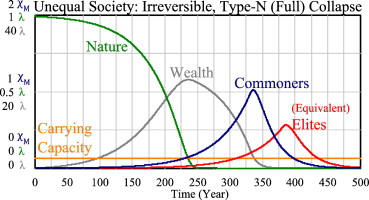
\includegraphics{fig/handy_unequal.jpg}

\emph{Motesharrei Memo}

n this paper we attempt to model collapse mathematically in a more
general way. We propose a simple model, not intended to describe actu-
al individual cases, but rather to provide a general framework that
allows carrying out ``thought experiments'' for the phenomenon of
collapse and to test changes that would avoid it. This model (called
HANDY, for Human and Nature DYnamics) advances beyond existing
biological dynamic population models by simultaneously modeling
two separate important features which seem to appear across so
many societies that have collapsed: (1) the stretching of resources due
to the strain placed on the ecological carrying capacity
and (2) the economic stratification of society into Elites and
Masses (or ``Commoners'')

HANDY is based on the classical predator--prey model, the
inclusion of two societal classes introduces a much richer set of dynam-
ical solutions, including cycles of societal and ecological collapse, as well
as the possibility of smoothly reaching equilibrium (the ecological car-
rying capacity). We use Carrying Capacity in its biological definition:
the population level that the resources of a particular environment
can sustain over the long term.

HANDY was
originally built based on the predator--prey model. We can think of
the human population as the ``predator'', while nature (the natural
resources of the surrounding environment) can be taken as the ``prey'',
depleted by humans. In animal models, carrying capacity is an upper
ceiling on long-term population. When the population surpasses the
carrying capacity, mechanisms such as starvation or migration bring
the population back down. However, in the context of human societies
the population does not necessarily begin to decline upon passing the
threshold of carrying capacity, because, unlike animals, humans can
accumulate large surpluses (i.e., wealth) and then draw down those re-
sources when production can no longer meet the needs of consumption.
This introduces a different kind of delay that allows for much more com-
plex dynamics, fundamentally altering the behavior and output of the
model. Thus, our model adds the element of accumulated surplus not
required in animal models, but which we feel is necessary for human
models. We call this accumulated surplus ``wealth''.

Empirically, however, this accumulated surplus is not evenly distrib-
uted throughout society, but rather has been controlled by an elite. The
mass of the population, while producing the wealth, is only allocated a
small portion of it by elites, usually at or just above subsistence levels.
Based on this, and on the historical cases discussed in the introduction,
we separated the population into ``Elites'' and ``Commoners'', and introduced
a variable for accumulated wealth.

This adds a different dimension of predation whereby
Elites ``prey'' on the production of wealth
by Commoners. As a result, HANDY consists of four prediction equations:
two for the two classes of population, Elites and Commoners,
denoted by \(x_E\) and \(x_C\) , respectively; one for the natural resources or
Nature, \(y\); and one for the accumulated Wealth, \(w\), referred to hereafter
as ``Wealth''. This minimal set of four equations seems to capture essential
features of the human--nature interaction and is capable of producing
major potential scenarios of collapse or transition to steady state.

A similar model of population and renewable resource dynamics
based on the predator--prey model was developed in the pioneering
work of Brander and Taylor (1998) demonstrating that reasonable
parameter values can produce cyclical ``feast and famine'' patterns of
population and resources.
The BT approach only models Population and Nature and
does not include a central component of these historical cases: economic
stratification and the accumulation of wealth.

We have found that including economic
stratification, in the form of the introduction of Elites and Commoners,
as well as accumulated Wealth, results in a much richer variety of solutions,
which may have a wider application across different types of societies.
HANDY's structure also allows for ``irreversible'' collapses, without
the need to introduce an explicit critical depensation mechanism into
the model.

A decline in the
price of a resource is usually thought to reflect an increase in the
abundance of that resource, but in fact, it often reflects that the resource is
simply being extracted more rapidly.

Over the long-term, per capita resource-use has
tended to rise over time despite dramatic technological advances in
resource efficiency.

\href{https://www.sciencedirect.com/science/article/pii/S0921800914000615}{Motesharrei (2014) Human and nature dynamics (HANDY)}
\href{pdf/Motesharrei_2014_HANDY_Human_and_Nature_Dynamics.pdf}{(pdf)}

\hypertarget{anthropocene}{%
\chapter{Anthropocene}\label{anthropocene}}

``Political ecology is the product of our inscription in the capitalocene.
Anthropocene is an idealist and ideological support of capitalism.''
(Matthew Fliesfeder)

\textbf{Note}

Canary Island Promotion:

\begin{verbatim}
We only know 20% of the Planet Earth     
Humans only make up 0.01% of terrestrial life  
We have only discovered 15% ofliving species
81% of the seabed is still unkown to us
\end{verbatim}

????

\href{https://l.facebook.com/l.php?u=http\%3A\%2F\%2Fwww.hellocanaryislands.com\%2F\%3Ffbclid\%3DIwAR0KpL92zBE9DSFFBBlR3nUzvBiOeg8A-GavXdo7iG3FkfXs-qQJkzABYSM\&h=AT1b3VHRAPNbUMsETBii684uDQXiUvMGYAb5RKmfj1-SBxcHO-WGcEUt0cMBKL-6pyGiar4PybInjdaW7O0uy9zyVKsxJvjDmeHz1S7mYi78gtfsKSbXok8nzY0\&__tn__=\%2Cd-UC\%2CP-R\&c\%5B0\%5D=AT08xUEPHg6AG1h8CijMYsvQsAewR1efrP3cTARQlOlbbp1OjjOS7l5EEWN56QpEr43eZMYLpDdxhfjtxcRvHu6q_-C91aQ5RmmiqVUDwPFBn4dyozTyAWj8qB_XR8d3SnApk8jDSA3i_XUfVH9WN1jKbjfjnlou5zK5C5yo0mjfWWyz9kt0JQMtww}{Canary Islands promotion}

\hypertarget{human-self-awareness}{%
\section{Human Self-Awareness}\label{human-self-awareness}}

\emph{Austin}

If it seems frivolous to propose the solution to our problems is some new `Age', as if such a thing might be produced to order, consider that the momentous recognition of the Anthropoceneis exactly the sort of event that might induce an Age. The crystallizing of the Anthropocene is a stunning milestone in the history of human self-awareness -- `Oh, I see, we're that big!' Big enough to change planetary processes. Big enough that Earth is not the immutable backdrop we assumed it to be. Possibly, the only feasible response to such a profound reappraisal of our context is an equiproportional change in human cognition and self-organization. Indeed, with simultaneous advances in Earth sciences and neurosciences, our sense of the world and of the brain we use to navigate it, is changing rapidly and dramatically, with us sandwiched in between. It is impossible to imagine that human beings will not be deeply changed by current events.

\href{https://channelmcgilchrist.com/articles/the-matrix-of-the-emissary/}{Austin (2021) The Matrix of the Emissary - Market Primacy and The Sustainability Cris\\
is}

\hypertarget{material-footprint}{%
\section{Material Footprint}\label{material-footprint}}

\hypertarget{mfa}{%
\subsection{MFA}\label{mfa}}

\emph{Abstract Krausman:}
The growing extraction of natural resources and the waste and emissions
resulting from their use are directly or indirectly responsible for human-
ity approaching or even surpassing critical planetary boundaries. A sound
knowledge base of society's metabolism, i.e., the physical exchange pro-
cesses between society and its natural environment and the production and
consumption processes involved, is essential to develop strategies for more
sustainable resource use. Economy-wide material flow accounting (MFA) is
a framework that provides consistent compilations of the material inputs to
national economies, changes in material stocks within the economic system,
and material outputs to other economies and the environment. We present
the conceptual foundations of MFA and derived indicators and review the
current state of knowledge of global patterns and trends of extraction, trade,
and use of materials. We discuss the relation of material use and economic
development and the decoupling of material use from economic growth in
the context of sustainable resource use policies.

\hypertarget{eu28-footprint}{%
\subsection{EU28 Footprint}\label{eu28-footprint}}

\emph{Abstract Giljum:}
In the context of the transformation toward a ``green economy,'' issues related to natural
resource use have rapidly increased in importance in European and international policy
debates. The large number of studies applying economy-wide material flow analysis
so far mostly produced aggregated national indicators, making the results difficult to
connect to policies, which are often designed for single sectors or consumption areas.
This paper provides a detailed assessment of the composition of EU's material foot-
print in its global context, aiming at identifying the main product groups contributing
to overall material consumption and specifying the geographical sources for the raw
materials required to satisfy EU's final demand. Based on multi-regional input--output
(MRIO) modeling, we apply production layer decomposition to assess supply chains
and their structural changes from 1995 to 2011. The global MRIO database used in this
study is EXIOBASE 3, which disaggregates 200 products and 163 industries, of which 33
represent material extraction sectors. By that means, we increase the level of detail to
a degree where policies can more easily connect to. We find that the generally grow-
ing material footprint of the EU was characterized by a dramatic shift regarding the
origin of raw materials, with the share of materials extracted within the EU territory
falling from 68 \% in 1995 to 35 \% in 2011. In 2011, raw materials extracted in China to
produce exports to the EU already contributed an equal share to EU's material footprint
as material extraction within the EU itself. Import dependency is most critical for the
material group of metal ores, with only 13 \% of all metals required as inputs to EU final
demand stemming from within the EU. Regarding product composition, construction
was confirmed as the most important sector contributing to the material footprint, fol-
lowed by the group of manufacturing products based on biomass. Materials embodied
in service sector activities together contributed a quarter to the total material footprint
in 2011, making services an important, but currently disregarded area for European
resource policies. We also find that supply chain structures became more complex over
time, with a growing part located outside the EU territory.

\href{https://www.annualreviews.org/doi/10.1146/annurev-environ-102016-060726}{Krausman (2017) MFA Material Flow Accounting}
\href{pdf/Krausman_2017_MFA.pdf}{(pdf)}

\href{https://journalofeconomicstructures.springeropen.com/articles/10.1186/s40008-016-0048-5\#Abs1}{Giljum (2016) MRIO Based Material Footprint Assessment}
\href{pdf/Giljum_2016_MRIO_based_Material_Footprint.pdf}{(pdf)}

Max Roser tweeted the following text: ``Material Footprint' is a terrible metric, but it is unfortunately used as one of the indicators of the UN's Sustainable Development Goals. A metric that allows you to offset the use of a ton of coal by using one less ton of sand should really not have that status.'' (1) In the following discussion he said that we should: ``stop reporting environmental impact in this way.'' (2) and that he finds ``Equal weights for fossil fuels and stones {[}\ldots{]} ethically absolutely horrible.'' (3) To make this point, he referred to a recent publication, comparing and disaggregating the EU's overall material footprint (MF) between 1995 and 2011, and more specifically, to one apparent substitution of clay and sand (decreased) with coal use (increased by roughly the same amount)

`Material Footprint' seems to me a bad metric for our impact on the environment.
Some resource use is much more harmful and to treat a kg of sand just like a kg of coal is a terrible idea.
To simply sum up their weight hides that resource use that has the worst impact.

The usefulness of aggregate material flow indicators: their purpose is to study the social metabolism, which is the material scale, composition, and pattern of the human-environment interaction

f we look beyond Roser's blanket rejection of MF and at available scientific publications, we find that MF is actually a useful proxy for aggregate environmental pressures. This is simply because all material extraction (be it biomass, metals, fossil fuels or non-metal minerals) has some impact (7). So, if we measure MF and environmental impacts separately, we would expect to find a correlation between the two. This is exactly what happens. MF is highly correlated with other indicators for environmental pressure, such as carbon dioxide and ecological footprint (6). Also, as Krausmann et al.~state (8, see also 9), material use (here domestic) correlates well with more complex indicators such as environmentally-weighted material use, accounting for different impacts of the respective material categories. Another reason why MF is a useful indicator is its simplicity while being representative.
Indeed, Steinmann et al.~(10) assessed 976 products and found that (p.~1) ``the resource footprints {[}here material (excl. energy and biomass), energy, land, and water{]} accounted for \textgreater90\% of the variation in the damage footprints. {[}\ldots{]} Our results indicate that relatively simple resource footprints are highly representative of damage to human health and biodiversity''. Finally, Voet et al.~(11) reach similar conclusions (p.~130): ``if we compare environmental impact with DMC {[}Domestic Material Consumption{]}, we can conclude that the contribution to the environmental pressure and the contribution to the DMC is not so different for these {[}resource{]} categories''. Thus, MF captures important connections between human extractive activity and environmental pressures quite well on an aggregate level, and this in a simple and understandable way.

\href{https://degrowth.org/2021/02/06/aggregate-material-footprint-as-a-proxy-for-environmental-pressures/}{Lorenz Keyser - Reply to Max Roser}

\citep[ Twitter Thread]{LorenzClimate}(\url{https://twitter.com/LorenzClimate/status/1357810876410175492})

\hypertarget{global-human-made-mass-exceeds-all-living-biomass}{%
\subsection{Global human-made mass exceeds all living biomass}\label{global-human-made-mass-exceeds-all-living-biomass}}

\emph{Memo:}

At the beginning of the twentieth century, anthropogenic mass was equal to only 3\% of global biomass.
About 120 years later, in 2020, anthropogenic mass is exceeding overall biomass in the world.

As the global effect of humanity accelerates, it is becoming ever more imperative
to quantitatively assess and monitor the material flows of our socioeconomic system,
also known as the socioeconomic metabolism.
This quantification is at the heart of the economy-wide material flow analysis framework,
under the field of industrial ecology, which is based on mass balance accounting.

Humanity has become a dominant force in shaping the face of Earth.
We are in the Anthropocene.
The overall living biomass on Earth currently equals approximately 1.1 teratonnes.
The anthropogenic mass has recently doubled roughly every 20years.
The Earth is exactly at the crossover point.
The antropogenic mass will surpass all other global living biomass in 2020.
Each week more than the bodyweight of all humans of antropogenic mass is produced.
This quantification of the human enterprise gives a mass-based quantitative and symbolic characterizatio

The global mass of of produced plastic is greater than the overall mass of all terrestrial and marine animals combined.

\begin{longtable}[]{@{}ll@{}}
\toprule
Living Biomass & Human-mademass\tabularnewline
\midrule
\endhead
Animals 4 Gt & Plastic 8 Gt\tabularnewline
Trees 900 Gt & Buildings 1100 Gt\tabularnewline
\bottomrule
\end{longtable}

The mass of humans is only about 0.01\% of global biomass.
Since the first agricultural revolution, humanity has roughly halved the mass of plant.
While modern agriculture utilizes an increasing land area for growing crops,
the total mass of domesticated crops (about 0.01 Tt)11 is vastly outweighed by
the loss of plant mass resulting from deforestation,forest management and other land-use changes.
These trends in global biomass have affected the carbon cycle and human health.
Additional human actions, including livestock husbandry, hunting and overfishing,
have also strongly affected the masses of various other taxa.

Continuous increases in anthropogenic mass, peaking at over 5\% per year,
mark the period immediately following World War II.
This period, frequently termed the `Great Acceleration',
is characterized by enhanced consumption and urban development

Quantifying the human appropriation of net primary production,
have focused on the allocation of the biosphere productivity flow for human usage.
The anthropogenic mass does not arise out of the biomass stock but from
the transformation of the orders-of-magnitude higher stock of mostly rocks and minerals.
In doing so, humanity is converting near-surface geological deposits into a socially useful form,
with wide implications for natural habitats, biodiversity, and various climatic and
biogeochemical cycles.

\href{https://www.nature.com/articles/s41586-020-3010-5.epdf?sharing_token=5BfrjXKSdktry3fKS7ssCdRgN0jAjWel9jnR3ZoTv0MLvUZ1C0L35yEQYHf_pwmiKx-xqIzWDg-_bH8WmUJdQjqDv1hJIWjUwOgpVde7Oc47mU9HfjoCpd8F0qewoXmjl6QNLlUMD2eeD21ompdgtw3j2FQ9z0hhBzCsqewC9BUQNhgBo5rYNFnTf9gTg419kTld3VXUhXOFlygv007wkcA8jVVlyrBd14KL3O0lNyCW54cq4jSFDWqF63iJKDWo_R6M1MFwDWk6OSU79I8W9ga2hbL-jY7gNoOR9LOhqUfR2c1P5oQrsITBs9UtutQEh--2BsxnLatS_s9_H68tUNKvlSYLF9xHfwWb-DXmoouJXov9L4EbWJH6itdSZHqa\&tracking_referrer=www.theguardian.com}{Nature article (shared pdf)}

\href{https://www.nature.com/articles/s41586-020-3010-5}{Nature web}

\href{https://github.com/milo-lab/anthropogenic_mass}{Github Code and Data}

\hypertarget{sand-mining}{%
\subsection{Sand Mining}\label{sand-mining}}

Sand crisis: mafias thrive as shortages loom.

Demand for construction sand is rising faster than supply, pushing even countries in the Middle East to import it from as far away as Australia and Canada.

Sand, a building block of modern life that sits at the heart of a destructive and sometimes illegal industry, is in increasingly short supply --- and nobody knows how soon it will run out.

Sand is the most used material on the planet but also one of the least well monitored. Unlike most other commodities, policymakers only have rough estimates of how much of it is used each year. A landmark report from the UN Environment Program (UNEP) in 2019 had to rely on data for cement --- which sand and gravel are mixed with to make concrete --- to land on a ballpark figure of 50 billion tons.

Sand mining destroys habitats, dirties rivers and erodes beaches, many of which are already losing ground to rising sea levels. When miners dig out layers of sand, riverbanks become less stable. The pollution and acidity can kill fish and leave less water for people and crops. The problem is made worse when dams upstream prevent sediments from replenishing the river.

\href{https://www.dw.com/en/sand-crisis-shortage-supply-mafia/a-56714226}{DW}

Desert sand grains are too smooth to be useful, and most of the angular sand that is suitable for industry comes from rivers (less than 1\% of the world's land)5. This extraction of sand and gravel has far-reaching impacts on ecology, infrastructure and the livelihoods of the 3 billion people who live along rivers

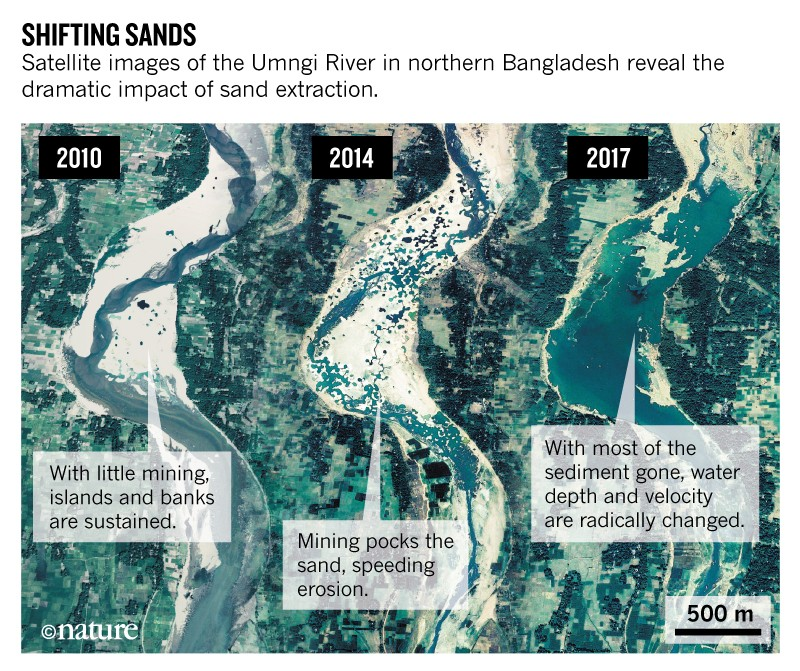
\includegraphics{fig/sand_mining_bangladesh.jpg}

Extraction of sand and gravel from active sources can cause great environmental, social and economic harm, whereas extraction from passive sources has fewer environmental impacts. For example, in the Mekong delta, the Vietnamese government estimates that nearly 500,000 people will need to be moved away from river banks that are collapsing as a result of sand mining in the channel. In the Ganges River in northern India, eroded river banks have destroyed the nesting and breeding habitats of fish-eating gharial crocodiles (Gavialis gangeticus), a critically endangered species with only around 200 adults left in the wild in northern India and Nepal.

\href{https://www.nature.com/articles/d41586-019-02042-4}{Bendixsen (2019) Nature}

\hypertarget{biodiversity}{%
\chapter{Biodiversity}\label{biodiversity}}

\begin{quote}
There is no way 8-10 billion people make it over the 2100 line with
half of plants \& insects at risk of extinction.
No way.
We're sawing through the trunk of the tree of life:
we will fall too.
(Julia Steinberger (Twitter))
\end{quote}

\begin{quote}
First Nations demand a say on climate change.
``Indigenous people make up less than 5\% of the world's population, but they manage and protect 80\% of global biodiversity.''
\href{https://www.theguardian.com/australia-news/2021/mar/27/we-want-to-be-included-first-nations-demand-a-say-on-climate-change}{Guardian}
\end{quote}

\hypertarget{economics-of-biodiversity}{%
\section{Economics of Biodiversity}\label{economics-of-biodiversity}}

\hypertarget{dasgupta-review-2021}{%
\subsection{Dasgupta Review 2021}\label{dasgupta-review-2021}}

The report proposes

\begin{verbatim}
- Recognising nature as an asset and  
- Reconsidering our measures of economic prosperity.
\end{verbatim}

Recommendations include:

\begin{verbatim}
- Making food and energy systems sustainable through technological innovations and policies that change prices and behavioural norms  
- Investing in programmes that provide community-based family planning  
- Expanding and improving access to protected areas  
- Implementing large-scale and widespread investment in nature-based solutions to address biodiversity loss  
- Introducing natural capital into national accounting systems.
\end{verbatim}

\href{https://www.bbc.com/news/science-environment-55893696}{Dasgupta Review (BBC)}

The Dasgupta Review is an independent, global review on the Economics of Biodiversity led by Professor Sir Partha Dasgupta (Frank Ramsey Professor Emeritus, University of Cambridge). The Review was commissioned in 2019 by HM Treasury and has been supported by an Advisory Panel.

\textbf{The Review calls for changes in how we think, act and measure economic success.}

The new framework presented by the Review sets out
how we should account for Nature in economics and decision-making.

The Review finds that humanity has collectively mis-managed its global portfolio of assets,
meaning the demands on nature far exceed its capacity to supply the goods and services
we all rely on.

\begin{quote}
Humanity must ensure its demands on nature do not exceed its sustainable supply and must increase the global supply of natural assets relative to their current level. For example, expanding and improving management of Protected Areas; increasing investment in Nature-based Solutions; and deploying policies that discourage damaging forms of consumption and production.
\end{quote}

.

\begin{quote}
We should adopt different metrics for economic success and move towards an inclusive measure of wealth that accounts for the benefits from investing in natural assets and helps to make clear the trade-offs between investments in different assets. Introducing natural capital into national accounting systems is a critical step.
\end{quote}

.

\begin{quote}
We must transform our institutions and systems -- particularly finance and education -- to enable these changes and sustain them for future generations. For example, by increasing public and private financial flows that enhance our natural assets and decrease those that degrade them; and by empowering citizens to make informed choices and demand change, including by firmly establishing the natural world in education policy.
\end{quote}

\emph{Reactionn from Mark Carney.}
Ecosystems that have more diverse natural assets are more productive, resilient and adaptable. Just as diversity within a financial portfolio reduces risk and uncertainty, greater biodiversity reduces risks and uncertainty within a portfolio of natural assets. As we awaken to the importance of natural capital, we need to place greater value on sustainability and biodiversity -- the precondition to solving the twin crises of biodiversity and climate.

\emph{Reactionfrom Christiana Figueres:}
It is less costly to conserve Nature than to restore it once it's damaged or degraded and provides the economic rationale for expanding and improving the management of protected areas. We can translate this idea into action by protecting 30\% of the planet by 2030. The Review lays the foundation for how to address the twin crises of biodiversity and climate.

\emph{Reaction from Andrew Haldane:}
Most of economics and economic policy has neglected the role of Nature and
underplayed the importance of biodiversity in protecting both Nature and, ultimately, us.

\emph{Reaction from James E. Hansen:}
Flourishing nature, restoration of a healthy climate, and economic well-being of all humanity can co-exist, but they require understanding. Dasgupta's Review helps us begin a journey, which will require decades.

\href{https://www.gov.uk/government/publications/final-report-the-economics-of-biodiversity-the-dasgupta-review/the-economics-of-biodiversity-the-dasgupta-review-reactions}{Dasgupta Review Reactions at Launch}

\textbf{Memo Dasgupta:}

While most models of economic growth and development recognise that Nature is capable only
of producing a finite flow of goods and services, the focus has been to show that technological
progress can, in principle, overcome that exhaustibility. This is to imagine that, ultimately,
humanity is `external' to Nature.
The Review develops the economics of biodiversity on the understanding that we -- and our
economies -- are `embedded' within Nature, not external to it. The Review's approach is based
firmly in what we know from ecology about how ecosystems function, and how they are
affected by economic activity, including the extraction of natural resources for our production
and consumption, and the waste we produce through these activities, which ultimately damages
ecosystems and undermines their ability to provide the services on which we rely. This approach
helps us to understand that the human economy is bounded and reshapes our understanding
of what constitutes truly sustainable economic growth and development: accounting fully for
the impact of our interactions with Nature and rebalancing our demand with Nature's capacity
to supply.

The change required should be geared towards three broad \textbf{transitions}:

\begin{enumerate}
\def\labelenumi{(\roman{enumi})}
\item
  Ensure that our demands on Nature do not exceed its supply,
  and that we \textbf{increase} (\emph{sic!!}) Nature's supply relative to its current level.
\item
  Change our measures of economic success to guide us on a
  more sustainable path.
\item
  Transform our institutions and systems -- in particular our
  finance and education systems -- to enable these changes and
  sustain them for future generations.
\end{enumerate}

Not so long ago, when the
world was very different from what it is now, the economic questions that needed urgent
response could be studied most productively by excluding Nature from economic models.
Nature entered macroeconomic models of growth and development in the 1970s, but in an
inessential form. 3 The thought was that human ingenuity could overcome Nature's scarcity over
time, and ultimately (formally, in the limit) allow humanity to be free of Nature's constraints.
But the practice of building economic models on the backs of those that had most recently been
designed meant that the macroeconomics of growth and development continued to be built
without Nature's appearance as an essential entity in our economic lives.

The natural world is studied in relation to the many other assets we
hold in our portfolios, such as the vehicles we use for transport, the homes in which we live,
and the machines and equipment that furnish our offices and factories. But like education and
health, Nature is more than a mere economic good. Nature nurtures and nourishes us, so we
will think of assets as durable entities that not only have use value, but may also have intrinsic
worth. Once we make that extension, the economics of biodiversity becomes a study in portfolio
management.

Finance plays a crucial role. A significant portion of the responsibility for helping us to shift
course will fall on the global financial system.

\textbf{To leave Nature alone so that it is able to thrive is to invest in it.}

The risks associated with biodiversity loss -- reductions in the productivity and resilience of
ecosystems along supply chains -- have significant macroeconomic and financial implications.
Far more global support is needed for initiatives directed at enhancing the understanding and
awareness among financial institutions of Nature-related financial risks, learning and building
on the advances on climate-related financial risks.

Central banks and financial supervisors can
support this by assessing the systemic extent of Nature-related financial risks. A set of global
standards is required. They should be underpinned by data that are both credible and useful for
decision-making. Businesses and financial institutions could then be obliged to integrate Nature-
related considerations with their other objectives. The idea ultimately is to have them assess
and disclose their use of natural capital. The Task Force on Nature-related Financial Disclosures,
(TNFD) established in 2020, is a step in that direction.

Integrating the protection of biodiversity with the fiduciary duties of
institutional investors and asset managers
would be a way to ensure their investment policies account for natural capital.

The time horizonwithin which financial actors plan and act is, unhappily (!!sic!!),
not more than a few years.
Financial regulators and supervisors can play a key role in the necessary shift
by changing their own assessment horizons and using their regulatory powers.

\emph{Moral Issue}
Ultimately though, it is we citizens who can bring about such changes. (!!sic!!)
Connecting with Nature needs to be woven throughout our lives.
The three pervasive features of Nature -- mobility, silence and invisibility --
mean that the consequences of actions
which desecrate Nature are often untraceable to those who are responsible.
We will have to rely also on self-enforcement, that is, be our own
judge and jury.

\textbf{Memo Main Report:}
Now we are plundering every corner of the world, apparently neither knowing or caring what
the consequences might be.

Today, we ourselves, together with the livestock we rear for
food, constitute 96\% of the mass of all mammals on the planet. Only 4\% is everything else --
from elephants to badgers, from moose to monkeys. And 70\% of all birds alive at this moment
are poultry -- mostly chickens for us to eat.

\emph{GDP}
The contemporary practice of using Gross Domestic Product (GDP) to judge
economic performance is based on a faulty application of economics. GDP is a flow (so many
market dollars of output per year), in contrast to inclusive wealth, which is a stock (it is the
social worth of the economy's entire portfolio of assets). Relatedly, GDP does not include the
depreciation of assets, for example the degradation of the natural environment (we should
remember that `G' in GDP stands for gross output of final goods and services, not output net
of depreciation of assets). As a measure of economic activity, GDP is indispensable in short-run
macroeconomic analysis and management, but it is wholly unsuitable for appraising investment
projects and identifying sustainable development. Nor was GDP intended by economists who
fashioned it to be used for those two purposes. An economy could record a high rate of
growth of GDP by depreciating its assets, but one would not know that from national statistics.

\textbf{VALUES}
Correct economic reasoning is entangled with our values. Biodiversity does not only have
instrumental value, it also has existence and intrinsic value, perhaps even moral worth.

\textbf{(Use) Value} vs \textbf{(Intrinsic) Worth} vs \textbf{(Social) Worth} vs \textbf{(Inclusive) Wealth}
Nature is more than a mere economic good. Nature nurtures and nourishes us,
so we will think of assets as durable entities that not only have use value, but may also have
intrinsic worth. Once we make that extension, the economics of biodiversity becomes a study in
portfolio management.

In order to judge whether the path of economic development
we choose to follow is sustainable, nations need to adopt a system of economic accounts that
records an inclusive measure of their wealth. \textbf{The qualifier \emph{inclusive} says that wealth includes
Nature as an asset.}

The contemporary practice of using Gross Domestic Product (GDP) to judge
economic performance is based on a faulty application of economics. GDP is a flow (so many
market dollars of output per year), in contrast to inclusive wealth, which is a stock (it is the
social worth of the economy's entire portfolio of assets)

\emph{Inclusive Wealth}
The accounting value of an economy's stock of capital goods is its inclusive wealth. The qualifier
signals that the notion of wealth adopted here differs from the one in common use in two ways:
(i) accounting prices are not necessarily market prices; and (ii) in addition to produced capital,
wealth includes human capital and natural capital. As accounting prices measure the social
worth of goods and services, the inclusive wealth of a nation is the social worth of its capital
goods. As noted previously, by `social worth' we mean not only the worth to people who are
alive at that date, but also to future people.

\textbf{Valueing Biodiversity}
Ecosystems are capital goods. Biodiversity is a characteristic of ecosystems. In the terminology
introduced in Chapter 1, it is an enabling asset.

Humanity's future will be shaped by the portfolio of \textbf{assets} we inherit and choose to pass on,
and by the balance we strike between the portfolio and the size of our population. \emph{Assets are
durable objects, producing streams of services}. Their durability enables us to save them for our
own future, offer them as gifts to others, exchange them for other goods and services, and
bequeath them to our children. Durability does not mean everlasting. Assets depreciate, but
unlike services they are not fleeting.

\emph{Capital Assets}
Perhaps because financial capital has figured prominently in
economists' writings, the qualifier `capital' is sometimes added to assets, as in `capital assets'.
Assets acquire their value from the services they provide over their remaining life

\emph{Wealth Accounts}
a deep connection
between inclusive wealth and intergenerational well-being. We prove that any change in one
is mirrored in a corresponding change in the other. The correspondence is named the wealth/
well-being equivalence theorem. We show that the theorem offers a way to judge whether the
development path an economy is following meets the requirement of sustainability. The theorem
is also shown to be the right criterion for evaluating public policy. Inclusive wealth is the coin
with which economic progress or its absence should be measured. Private companies prepare
balance sheets. The theorem shows why countries should now prepare wealth accounts.

\textbf{Capital Goods} vs \textbf{Enabling Assets}
In our classification, there are thus three categories of capital goods and
a wide range of enabling assets.
Three-way partition of \emph{capital goods}: produced capital (buildings, roads,
ports, machines, instruments), human capital (population size, health, education, reputation,
knowledge and skills) and natural capital (ecosystems, sub-soil resources).
What remains -- institutions and practices, more generally, social capital, and
publicly available knowledge --
we will call \emph{enabling assets},
because they confer value to the three classes of capital goods by facilitating their use.

** Economic Evaluation**
Management of a society's portfolio of assets involves
policy analysis and
sustainability assessment.
We call the two generically as economic evaluation.

\emph{(Green Book 6.48)}
A focus solely on the marginal valuation of a loss in services may overlook the potential
for large reductions in stocks.

\emph{Pollinators}
At smaller levels of aggregation, total values of Nature's services can be meaningful and yet not
be useful for policy. It is tempting, for example, to cite the estimate that pollination contributes
an annual £510-690 million to the UK's agricultural production as providing a reason for
restoring the population of pollinators (Breeze, Roberts, and Potts, 2012). But should we regard
it to be a large or small figure? Based on 2019 data from the UK Office of National Statistics,
as a proportion of the UK's annual agricultural output, it is approximately 5\%. As a proportion
of the UK's GDP, it is 0.03\%, a negligible figure. So why care whether any pollinators are left?
The reason we should not be dismissive of pollinators is that proportional figures do not signal
worth. National asset management requires that pollinators enter projects with their accounting
prices. Chapters 2 to 4 demonstrate that pollinators may be of great value even if their
measurable services to GDP are of negligible worth.

\href{https://www.gov.uk/government/publications/final-report-the-economics-of-biodiversity-the-dasgupta-review}{Dasgupta Review Final Report}
\href{pdf/Dasgupta_2021_Final.pdf}{(pdf final (full) report)}
\href{pdf/Dasgupta_2021_Short.pdf}{(pdf short)}
\href{pdf/Dasgupta_2021_Messages.pdf}{(pdf messages)}
\href{pdf/Dasgupta_2021_Interim.pdf}{(pdf Interim Report (April 2020))}

\href{https://tnfd.info/}{TNFD}

\textbf{Observations}

Borgelig idealisme

Document Searches:
`capitalism': 2 entries\\
`doughnut': 0

\href{https://www.worldeconomicsassociation.org/newsletterarticles/the-dasgupta-review/}{WEA Commentary}

\hypertarget{daggupta-review-deconstructed}{%
\subsection{Daggupta Review Deconstructed}\label{daggupta-review-deconstructed}}

\emph{Spash Abstract}

The Dasgupta Review is the latest attempt at justifying financialisation of
Nature, but also much more. It represents a high point in applying concepts
of capital and wealth accumulation comprehensively to all aspects of human
and non-human existence. Unravelling the flaws in the arguments,
contradictions and underlying motives requires both understand of and
cutting through the specialist language, neoclassical economic models,
mathematics and rhetoric. We offer a critical guide to and deconstruction of
Dasgupta's biodiversity economics and reveal its real aim. Framing critical
biodiversity loss as an issue of asset management and population size is a
blind to avoid questioning economic growth, which remains unchallenged
and depoliticized despite apparently recognizing natural limits. Dasgupta
ignores long-standing problems with capital theory and social cost--benefit
analysis. Rather than a scientific review of biodiversity economics he offers
impossible to achieve valuation, based on old flawed theories and methods,
embedded in an unsavoury political economy.

\emph{Spash Memo}

There is no error in this `independent' report having been commis-
sioned by the Treasury department under a ruling Conservative Party. While pricing, trading-off
and optimizing are traditional economic fare, the political vision here involves a far reaching public
policy agenda, promoting the total domination of non-financial aspects of life by finance.

Central to Dasgupta's whole approach is an analogy between biodiversity protection and finan-
cial asset management. Destruction of Nature is blamed on a misallocation of capital investment,
with too much going to produced and human capital relative to natural capital. Curbing biodiver-
sity destruction is then reframed as optimal asset management by a `citizen investor' guided by
`accounting prices' that correct all market failures by internalizing externalities after calculations
made by experts in social cost--benefit analysis.
Cost--benefit analysis is a calculus for maximizing an economy's inclusive wealth'. This
builds on the UN supported study entitled The Economics of Ecosystems and Biodiversity (TEEB,
2010) that moved from monetary valuation to capturing value via new financial instruments,
and linked directly into proposals to `hardwire biodiversity and ecosystems services into finance'
(UNEP Finance Initiative, 2010).

On this basis, and supported by powerful institutions and lobby groups, The Review places mon-
etary valuation of Nature at the forefront of national and international environmental policy. The
world is turned upside-down, so that wealth accumulation, sustainable growth (=development) and
`the economy' are the things in need of being protected, not Nature or biodiversity.

The Review in its full 610 page version is a user unfriendly technical report packed with standard
neoclassical economic (mathematical) models, annexes and specialist terminology, but the
abridged 100 page version misguides as to the problems underlying The Review and its failings.

\begin{quote}
Financial asset management is an
inappropriate analogy for biodiversity conservation.
\end{quote}

While ostensibly about biodiversity loss The Review is in fact a broad reaching orthodox econom-
ist's vision of how the entire world should operate. Humans are consumers who aim to maximize
their utility, which can be variously described as happiness, welfare or (Dasgupta's preference) well-
being. Despite claims that the model is not restricted to `individuals', that is exactly what is done,
because the `economic agent' -- regardless of whether a generation, government or family -- is an
identical optimizing unit. This agent is only concerned to maximize utility, which through a series
of equivalents becomes money; that is, utility = well-being = wealth = capital = money values.

Intergenerational well-being is defined as a function of four factors: consumption, investment in
human capital, investment in technological innovation and extraction of natural resources. How-
ever, the overarching objective is to maximize intergenerational well-being deemed equivalent to
inclusive wealth.
Maximizing inclusive wealth is considered to auto-
matically maximize intergenerational well-being which is then framed as the objective of policy-
making. Dasgupta terms this his `sustainable development theorem'

Dasgupta talks of `the economy' (a phrase used 91 times) in the singular, as if only his chosen
economic system could exist -- an idealized market capitalism. All variety in actual social provision-
ing systems and alternatives across time and space are conveniently ignored. Also absent from the
picture are corporations, one of the most powerful institutions in the modern economy, and the role
of organized labour unions. What is recognized is that `the economy' suffers imperfections because
prices fail to reflect social values. This means government intervention must be allowed, although
Dasgupta repeatedly emphasizes its dangers and especially market distorting (as opposed to market
correcting!) subsidies. The question then becomes what form government intervention should take?
Addressing market failures is the job of what is in effect a central planner, but presented in the
guise of a female `citizen investor' or `social evaluator'.
Governance for Dasgupta is about optimal
investment in capital assets. Nature is something that gives a rate of return and that economists have
failed to adequately include in their investment portfolios.
He repeatedly remarks that: `The fault is
not in economics; it lies in the way we have chosen to practise it'

That price-making markets fail to value things that matter to humans, and non-humans, is
reduced down to accountancy, getting the prices right and social CBA.
For Dasgupta the term `accounting prices' is substituted for the traditional economic terms
social cost or shadow prices.

The favoured mainstream economic accounting convention is
employed to calculate net present values assuming all future humans will be better-off in terms
of having more consumption. Dasgupta -- like other mainstream economists such as Nordhaus
and Stern -- relegates the fate of the future to a theoretical dispute over discount
rates.

\begin{quote}
In summary, Dasgupta is proposing the optimal management of life on Earth in all its facets, an
all encompassing approach, made possible by assuming the only thing that matters is maximizing
social value measured as monetary wealth invested in a capital stock. The aim of life is to maximize
rates of return on investments. Achieving social good requires that the wise `citizen investor' choose
the optimal portfolio of capital assets.
\end{quote}

\begin{quote}
This means Dasgupta's approach to everything -- human fertility, education, trust in
society, species existence, the sacred in indigenous communities, ecosystem structure and function
-- is reduced down to the value of capital and returns on capital investment.
\end{quote}

\textbf{Produced Capital}

As a neoclassical economist, Dasgupta opts for (ii), claiming that: `{[}a{]}ssets acquire their value from
the services they provide over their remaining life' (Dasgupta, 2021, p.~138). This leads to an asset management approach.
Different types of assets, or forms of capital, are required to produce the
same rate of return in order to achieve an optimally managed investment portfolio (i.e.~that maximizes
returns by equating returns on every investment at the margin). More simply, this means whether
investing in produced capital, education or blue whales the economic agent (`citizen investor')
seeks the same return. What is ignored by Dasgupta is a long history, that involved his own University
and Economics Department, concerning problems with measuring capital.

A further problem, largely unrecognized by most economists (from either Cambridge or else-
where), arises due to environmental pollution. As has been explained, capital is a monetary value
dependent either on its cost of production or the value of what it produces. However, those costs
and future return values are only valid for economic resource allocation if they take into account
all associated social costs and benefits in the production and consumption process. Due to the all per-
vasive character of pollution that means all prices must be adjusted, but to what and by whom? If no
objective value exists then economic theory cannot justify prices as valid reflections of a `true' social
value, let alone tell us what is the stock (i.e.~value) of produced capital, or any other capital.
The Dasgupta Review provides an excellent example of the contradictions and how economists
attempt to fudge all these issues. Dasgupta acknowledges the essential and central role of a common
metric for his capital approach:
It is not enough to say that houses can be measured in physical units (floor space, say), they need to be
compared with other capital goods, such as cars. We need a common unit. Valuing assets is a way to do
that. (Dasgupta, 2021, p.~323)
However, he is also repeatedly forced to admit the practical problems of valuing things and the
capital stock in particular. Yet, he assumes some social evaluation process will take care of
finding the `true price' by valuing everything in a money metric. Social CBA will be conducted
by expert economists, or a `social evaluator' nay `citizen investor', who will miraculously solve
all problems. \emph{Faith enters by the door and science leaves by the window.}

\textbf{Natural Capital}

Dasgupta (2021, p.3) states that: `In the Review, the terms Nature, natural capital, the natural
environment, the biosphere, and the natural world are used interchangeably'. More simply all con-
cepts of Nature are reduced to capital. Natural capital is an anthropocentric and utilitarian view of
Nature, where Nature is reframed as contributing goods and services solely for human well-being
(Hache, 2019). In The Review, ecosystem services are classified, following the Common Inter-
national Classification of Ecosystem Services (see Haines-Young \& Potschin, 2018), as either:

\begin{itemize}
\tightlist
\item
  Provisioning services: plants and animals for nutrition, materials or energy;
\item
  Regulating and maintenance services: such as habitat and gene pool protection, flood control,
  pest and disease control; or
\item
  Cultural services: covering intangible things such as the enjoyment and spiritual value of Nature.
\end{itemize}

Anything that fails to contribute to human well-being is ignored, deemed worthless, which again
places valuation at the centre of the whole approach.

Even if the, so called, stock of natural capital were known in physical terms it would, like produced
capital, require a common value basis to make diverse elements comparable and commensurate.
Numbers may be produced, as under existing `experimental' approaches (e.g.~Office for National
Statistics, 2020), but aggregate numbers for national accounting do not help optimum portfolio
investment (i.e.~indicate rates of return on different investments). They also fail to meet the requirements of the neoclassical economic approach for scarcity prices of resources, the `true' social values,
called `accounting prices' by Dasgupta. Those values, as Dasgupta repeatedly tells us, cannot be
found in any market. As he makes clear:
Only social cost-benefit analysis, using the same accounting prices as are estimated for sustainability
assessment, would tell the social evaluator which investment projects are socially desirable.
Decades ago environmental CBA developed a range of methods for imputing monetary values, but
with limited applicability under specific conditions (Hanley \& Spash, 1993; Spash, 2005). For a
start, these methods only apply to marginal changes in environmental goods or services, not
least because the value of money itself (its marginal utility) alters when there are large changes
affecting income; also, economic welfare measures assume other things (e.g.~all other prices) remain
the same which is violated by large changes. Clearly things like mass extinction of species and
human induced climate change are not small, marginal, changes.

There are two major failings in The Review when valuing natural capital. First is the inability of
economists to actually apply their utility preference value theory to obtain `true' social costs (Das-
gupta's accounting prices). Second is the divorce between the economic theory of value and a range
of alternative value theories held to exist in human societies.

An even more basic problem, with appealing to human preferences, occurs when people do not
understand complex environmental issues, or terminology (e.g.~biodiversity), or have never
encountered a species or know nothing of the object of value (e.g.~genes, microbes or distant eco-
systems). The problems with respect to biodiversity have long been recognized.

However, many economists, including Dasgupta, naïvely refer to establishing `true values'
as if people had, stored away in their brains, values to every entity on the planet in every quantity
and quality in which it might appear in an economic equation to be traded-off against something
else, and that they can immediately produce such values on demand when asked their maximum
willingness-to-pay (for or against an environmental change).

Then there is the disconnect between marginal values sought by social CBA and the aggregate
national income accounts covering the entire stock of natural capital.
The study Dasgupta takes as exemplary is by Managi and Kumar on `inclusive wealth' for a total
(not marginal productivity) value. Even this proves problematic. We are told that due to `data limit-
ations' natural capital was taken to be minerals and fossil fuels, agricultural land, forests as sources
of timber and fisheries. The topic of biodiversity is totally absent. Instead of social values (aka
accounting prices) we have a list of rather simple marketed inputs to production and consumption
using market prices. Both theory and relevance go out the win-
dow, once again. As Dasgupta's rhetoric rises, the failure of theory to translate into practice
becomes transposed into theory acting as a surrogate means by which to justify cutting corners.

As Dasgupta's rhetoric rises, the failure of theory to translate into practice
becomes transposed into theory acting as a surrogate means by which to justify cutting corners.
In practice, empirical corners have to be cut. An understanding of the tight {[}sic{]} theory helps accoun-
tants to justify the corners they choose to cut.
He then goes on to explain that:
\textgreater Moreover, there are Nature's objects and sites of cultural significance that resist being valued and placed
in comparison to marketed goods. Societies record their presence and allocate funds to preserve and
restore them. They fall outside the scope of national accounts. (Dasgupta, 2021, p.~337)

What then are the implications of recognizing the existence of things `that resist being valued and placed
in comparison to marketed goods'? Apparently nothing! The divorce from, and applicability to, reality
of Dasgupta's theory is for him irrelevant because `{[}e{]}mpirical work is forced to cut theoretical corners'.

Yet, despite the problems and contradictions Dasgupta implies all barriers to monetary valuation
can be overcome. Of course they must be, if his sustainability theorem, is to progress into policy:

\begin{quote}
economic worth of natural capital remains the greatest barrier to an understanding of economic devel-
opment. Until that ignorance is lifted, policy analysis will remain crippled and sustainability will continue to be a notion we admire but cannot put into operation. (Dasgupta, 2021, p.~353)
\end{quote}

He is correct that his policy analysis is indeed crippled. However, that policy analysis can be con-
ducted without his approach seems to pass him by, along with the impossibility of ever actually
implementing anything close to what he suggests, regardless of how many theoretical corners he
is prepared to cut.

The idea that time with a dying loved one, a non-
human species, an ecosystem or anything else cannot be valued in this way is highly problematic for
such economic accountancy, as adopted by Dasgupta, so it must be relegated to irrelevance by side-
lining (his favourite tactic). Mention something and its importance and then go about your econ-
omic business as normal. The result is to totally ignore plural values and alternative (non preference
utilitarian) systems of ethics as having any relevance to how `the economy' should be run or Nature
valued.

The basic fact is that if significant things cannot be valued as proposed, either due to inadequate
methods or existence of plural incommensurable values, then the whole approach of The Review
falls apart, along with neoclassical value theory. Money is used to create the illusion of a common
metric. As we saw for the case of produced capital, the only sense to be made of such a singular
concept as capital is to convert it to a common value basis. Whether returns to natural capital
or the total stock of natural capital, there must be some means of summing-up everything that con-
stitutes capital, which is impossible in physical terms. More frogs do not equate to fewer tigers.
What then is `natural capital'? Without the money metric it is non-existent, a meaningless econ-
omic abstraction totally divorced from reality. The myth of optimal resource management directing
environmental policy is then dead.

Biodiversity is described as `a characteristic of natural capital {[}\ldots{]} a factor influencing the pro-
ductivity of natural capital, or more concretely, ecosystems'. It is reduced
down to an input to production, something that adds productivity to natural capital. Dasgupta claims
that because biodiversity is only an enabling asset there is no need to measure its value directly.

Exactly why Dasgupta wants to relegate biodiversity to a more functionary sub-role is unclear.

Research from the early
1990s onwards uncovered was that people, when asked to state their preferences, may, in significant
numbers, reject the economists valuation approach and instead hold multiple and
incommensurable values.
They may hold rights-based positions and refuse to trade-off values.

This economics fails to empower ecologists, respect Nature, pay attention to
biodiversity science or even listen to what people say
when interviewed; it has been doing exactly the opposite.

\emph{OptimalExtinction}

Preserving any species, or anything, that
does not payback profit at the going commercial rate is inefficient.
All slow growing species should
be optimally and efficiently terminated. The stock should be liquidated and the capital invested else-
where.

We should remember Dasgupta's words, that: `Ecosystems are capital goods, like pro-
duced capital (roads, buildings, ports, machines)', while `Biodiversity is a characteristic of
ecosystems.

As Dasgupta himself makes very clear:

\begin{quote}
An asset that has a lower rate of return than another will not be chosen. A portfolio is the best for the agent only if the assets in it have the same rate of return.
\end{quote}

Quite simply, much of Nature is a bad investment and should be eradicated because financial returns
are higher elsewhere, and this financial profiteering is exactly how capitalism has been operating for
centuries and why we confront an ecological crisis. Dasgupta's capitalist approach to Nature does not
preserve anything, it simply makes investors' money, it accumulates financial capital. Biodiversity
valued as a financial asset will be destroyed, not saved, by Dasgupta's capitalist approach.

\emph{Population Growth}

The Review puts great emphasis on the size of the global population, in the tradition of Malthus,
while insisting that it does not. As Fletcher notes:

\begin{quote}
the interrelation between social inequality and ecological destruction can be explained in one of two
ways: as a function of human population growth creating resource scarcity; or as a product of a capi-
talist economic system demanding unsustainable resource use to facilitate economic growth that has
little to do with satiating the needs of the human collective, but rather with enriching a select few at
the expense of the rest---as well as at the expense of the planet as a whole.
\end{quote}

The Review clearly chooses the first. The focus on global population size, natality rates and poor
women's education implicitly shifts responsibility and blame for biodiversity loss away from capital
accumulation and on to developing countries and women.

\textbf{Biodiversity conservation is not asset management}

Dasgupta equates biodiversity conservation with asset management. The ana-
logy attempts to avoid structural change and maintain the current economic system with relatively
minor adjustments. This asset misallocation framing of biodiversity loss enables the continuation of
economic growth subject to an added condition of (hopefully) not destroying life on Earth.

Dasgupta tries to claim all conservation requires investment. In fact, Nature can regenerate with-
out human intervention (which in modernity is often the cause preventing this from occurring).
Where ecosystem restoration involves opportunity costs to curb destruction, the aim is not a return
on an investment. Preventing the destruction of Nature concerns stopping harm. Neither is pre-
venting harm to others (human or non-human) a matter of profiteering or accumulating wealth.
The view that biodiversity destruction is an issue of bad asset management is therefore far from
self-evident and on the contrary quite controversial. The more prevalent and contrasting view is
that biodiversity destruction has always been a corollary of capital accumulating growth, since such
economic activities are about appropriation and transformation of natural resources.

The analogy claims price-making markets are efficient, able to price scarce resources and allocate
them optimally. Public policy is seen as fostering new environmental markets to provide the `right
incentives' for private actors to choose the optimal allocation of resources that would maximize and
sustain economic growth. This aligns neoclassical economics with the neoliberal Wall Street Consen-
sus that seeks to transform the State from a sovereign actor to a standard setter, provider of subsidies
and means of de-risking private sector investment. That markets cannot achieve efficient allocation is
why Dasgupta requires a `social evaluator' and accounting (shadow) prices based on social CBA.

While Dasgupta highlights government subsidies, as a key market failure,
he ignores oligopoly and monopoly power as actualized today in the Davos elite of billionaires and
institutionalized in the multi-national corporation.

An asset manager's job is to maximize the return on a portfolio for a given investment mandate
allowing for risk taking. Optimization, whether of financial returns, or well-being, reduces human
action to pushing the limits and regulatory constraints to achieve maximum exploitation of others
(human and non-human) in order to make profit; what Kapp (1978/1963) termed cost-shifting.
When exploiting Nature and destroying biodiversity it assumes implicitly, and incorrectly, that
sufficiently complete and certain knowledge exists to avoid high stakes failures and catastrophic out-
comes. Crucially, optimizing reduces the margin for error and increases the risk of failure. Nature, by
contrast, avoids optimization and is full of redundancies, that make for resilience and robustness.

\textbf{Uncertainty}

Distinguishing between different types of unknown futures is important to understanding what
actions should be undertaken. Typically economists reduce all unknowns to risk, which is the prob-
ability of an event occurring. So when considering a simple coin toss, for example, we can expect a
50:50 chance of heads or tails and then repeatedly toss the coin to see. In this case the possible
future states or events are known and so are the probabilities. However, uncertainty and incertitude
arise when we either only know the possible outcomes, but not their probability, or we know the
risk, but not all the potential events. Human induced climate change is a good example, where
future states involve unique events, such as the melting of the West Antarctic ice sheets, an unre-
peatable experience, a knowable event without a probability distribution. We suffer from both par-
tial ignorance and social indeterminacy, not least because humans are also unpredictable in their
actions which may confound expectations. An important distinction is then that between weak
uncertainty where events and probabilities can be assigned (Spash, 2002a, Chapter 4), and strong
uncertainty where ignorance and indeterminacy dominate (Spash, 2002a, Chapter 5). The latter
requires a different approach to public policy that entails precaution (Stirling, 2017), not risk man-
agement or risk taking. Yet, despite these distinctions having been recognized a century ago by Key-
nes (1988/1921), economists, like Dasgupta, Stern, Nordhaus and others, persist in reducing strong
to weak uncertainty. While asset management and financial markets are generally designed to
handle risk, they are unable to handle strong uncertainty. In fact, the greater strong uncertainty
the more uncertain are the prices and the greater the chance of sudden and unexpected price
crashes (Slovik, 2011). This inability to deal with strong uncertainty makes the asset management
analogy both erroneous and dangerous. The analogy encourages misleading impressions of
substitutability and lognormal probability distributions, a false sense of predictability and promotes
inappropriate financial concepts (such as diversification).

Asset management is a profession where there is a huge gain/lose asymmetry in decision-mak-
ing, i.e.~between potential gain and personal risk. Rewards are typically a function of both the quan-
tity of assets under management and over-performance, but when asset managers fail they can only
lose their job. They are incentivised by design to take a great deal of risk. The analogy implies this
type of hugely asymmetric pay-off and limited accountability is the appropriate model to be
adopted by policy-makers, Dasgupta's citizen investor. The psychology of a high stakes gambler
hardly seems an ideal for public policy, especially where responsibility extends to existential threats
to others (both non-human and human).

The psychological aspect of financial markets involves group behaviour creating instability. For
example, the much-praised benefits of diversification (i.e.~risk spreading) evaporate when a big crises
hits, because fear dominates behaviour (all correlations jump towards one). The `risk appetite' of
market participants disappears, and trading positions are closed to stop losses or lock-in profits in
assets unrelated to the original event. This exemplifies how financiers' behaviour is dominated by
interdependent expectations. Keynes (1978/1936, p.~156) described professional investment as like
a newspaper competition in which the competitors have to pick out the six prettiest faces from a hun-
dred photographs, the prize being awarded to the competitor whose choice most nearly corresponds
to the average preferences of the competitors as a whole. You win not by judging who has the prettiest
face, but by guessing whom others on average will likely think has the prettiest face, while they guess
how you (and others) think they will think, and you guess how they think you (and others) will think,
and so on. Investment is game-playing not truth seeking. It requires very different skills from Nature
conservation or biodiversity preservation, where traditional and scientific knowledge provide causal
descriptive understanding of biophysical structure that informs social practice.

\textbf{Conclusions}

The fact that governments have budgetary choices and trade-offs to make does not imply, in any
way, that environmental policies are similar to asset management.

Using the language and concepts of finance and
capitalism to describe loss of biodiversity is far from neutral,
certainly not scientific let alone objective, and misunderstands the object of concern.

Promoting such
an incorrect framing is deeply problematic and worrying, because it will not only misdirect public
policy on biodiversity loss but also fail to address the structural causes of the ongoing
social-ecological and economic crises facing humanity.

\href{https://www.tandfonline.com/doi/full/10.1080/14747731.2021.1929007}{Spash (2021) The Dasgupta Review deconstructed: an exposé of biodiversity economics}
\href{pdf/Spash_2021_Dasgupta_Deconstructed.pdf}{(pdf)}

\hypertarget{invasive-species}{%
\section{Invasive Species}\label{invasive-species}}

\hypertarget{trade-related-costs}{%
\subsection{Trade related Costs}\label{trade-related-costs}}

\emph{Carrington}

The costs of damage caused by invasions of alien species across the world
is trebling every decade, research has found.

Mosquitoes, rats, ragweeds and termites are among the species that have hitched a ride on globalised trade routes, bringing disease, crop destruction and damage to buildings. The scientists calculated the costs at \$1.3tn (£944bn) since 1970, and said even this ``staggering sum'' was likely to be a big underestimate as much damage is unreported.

\href{https://www.inkl.com/news/damage-from-alien-species-invasions-trebling-every-decade?share=EQBnNnUMdyY}{Carrington (2021) Damages from Invasive Species Trebling}

\emph{Diagne}

Biological invasions are responsible for substantial biodiversity declines as well as high economic losses to society and monetary expenditures associated with the management of these invasions1,2. The InvaCost database has enabled the generation of a reliable, comprehensive, standardized and easily updatable synthesis of the monetary costs of biological invasions worldwide3. Here we found that the total reported costs of invasions reached a minimum of US\$1.288 trillion (2017 US dollars) over the past few decades (1970--2017), with an annual mean cost of US\$26.8 billion. Moreover, we estimate that the annual mean cost could reach US\$162.7 billion in 2017. These costs remain strongly underestimated and do not show any sign of slowing down, exhibiting a consistent threefold increase per decade. We show that the documented costs are widely distributed and have strong gaps at regional and taxonomic scales, with damage costs being an order of magnitude higher than management expenditures. Research approaches that document the costs of biological invasions need to be further improved. Nonetheless, our findings call for the implementation of consistent management actions and international policy agreements that aim to reduce the burden of invasive alien species.

\href{https://www.nature.com/articles/s41586-021-03405-6}{Diagne (2021) High and rising economic costs of biological invasions worldwide. Nature (Paywall)}

\hypertarget{degradation-loss}{%
\section{Degradation Loss}\label{degradation-loss}}

\emph{Ellis Significance}

The current biodiversity crisis is often depicted as a struggle to preserve untouched habitats. Here, we combine global maps of human populations and land use over the past 12,000 y with current biodiversity data to show that nearly three quarters of terrestrial nature has long been shaped by diverse histories of human habitation and use by Indigenous and traditional peoples. With rare exceptions, current biodiversity losses are caused not by human conversion or degradation of untouched ecosystems, but rather by the appropriation, colonization, and intensification of use in lands inhabited and used by prior societies. Global land use history confirms that empowering the environmental stewardship of Indigenous peoples and local communities will be critical to conserving biodiversity across the planet.

\emph{Ellis Abstract}

Archaeological and paleoecological evidence shows that by 10,000 BCE, all human societies employed varying degrees of ecologically transformative land use practices, including burning, hunting, species propagation, domestication, cultivation, and others that have left long-term legacies across the terrestrial biosphere. Yet, a lingering paradigm among natural scientists, conservationists, and policymakers is that human transformation of terrestrial nature is mostly recent and inherently destructive. Here, we use the most up-to-date, spatially explicit global reconstruction of historical human populations and land use to show that this paradigm is likely wrong. Even 12,000 y ago, nearly three quarters of Earth's land was inhabited and therefore shaped by human societies, including more than 95\% of temperate and 90\% of tropical woodlands. Lands now characterized as ``natural,'' ``intact,'' and ``wild'' generally exhibit long histories of use, as do protected areas and Indigenous lands, and current global patterns of vertebrate species richness and key biodiversity areas are more strongly associated with past patterns of land use than with present ones in regional landscapes now characterized as natural. The current biodiversity crisis can seldom be explained by the loss of uninhabited wildlands, resulting instead from the appropriation, colonization, and intensifying use of the biodiverse cultural landscapes long shaped and sustained by prior societies. Recognizing this deep cultural connection with biodiversity will therefore be essential to resolve the crisis.

\emph{Ellis Memo}

\textbf{Natural History Is Human History}

Contemporary patterns of biodiversity-rich areas, areas priori-
tized for conservation, and those specifically labeled ``natural'' all
show long and significant histories of human use

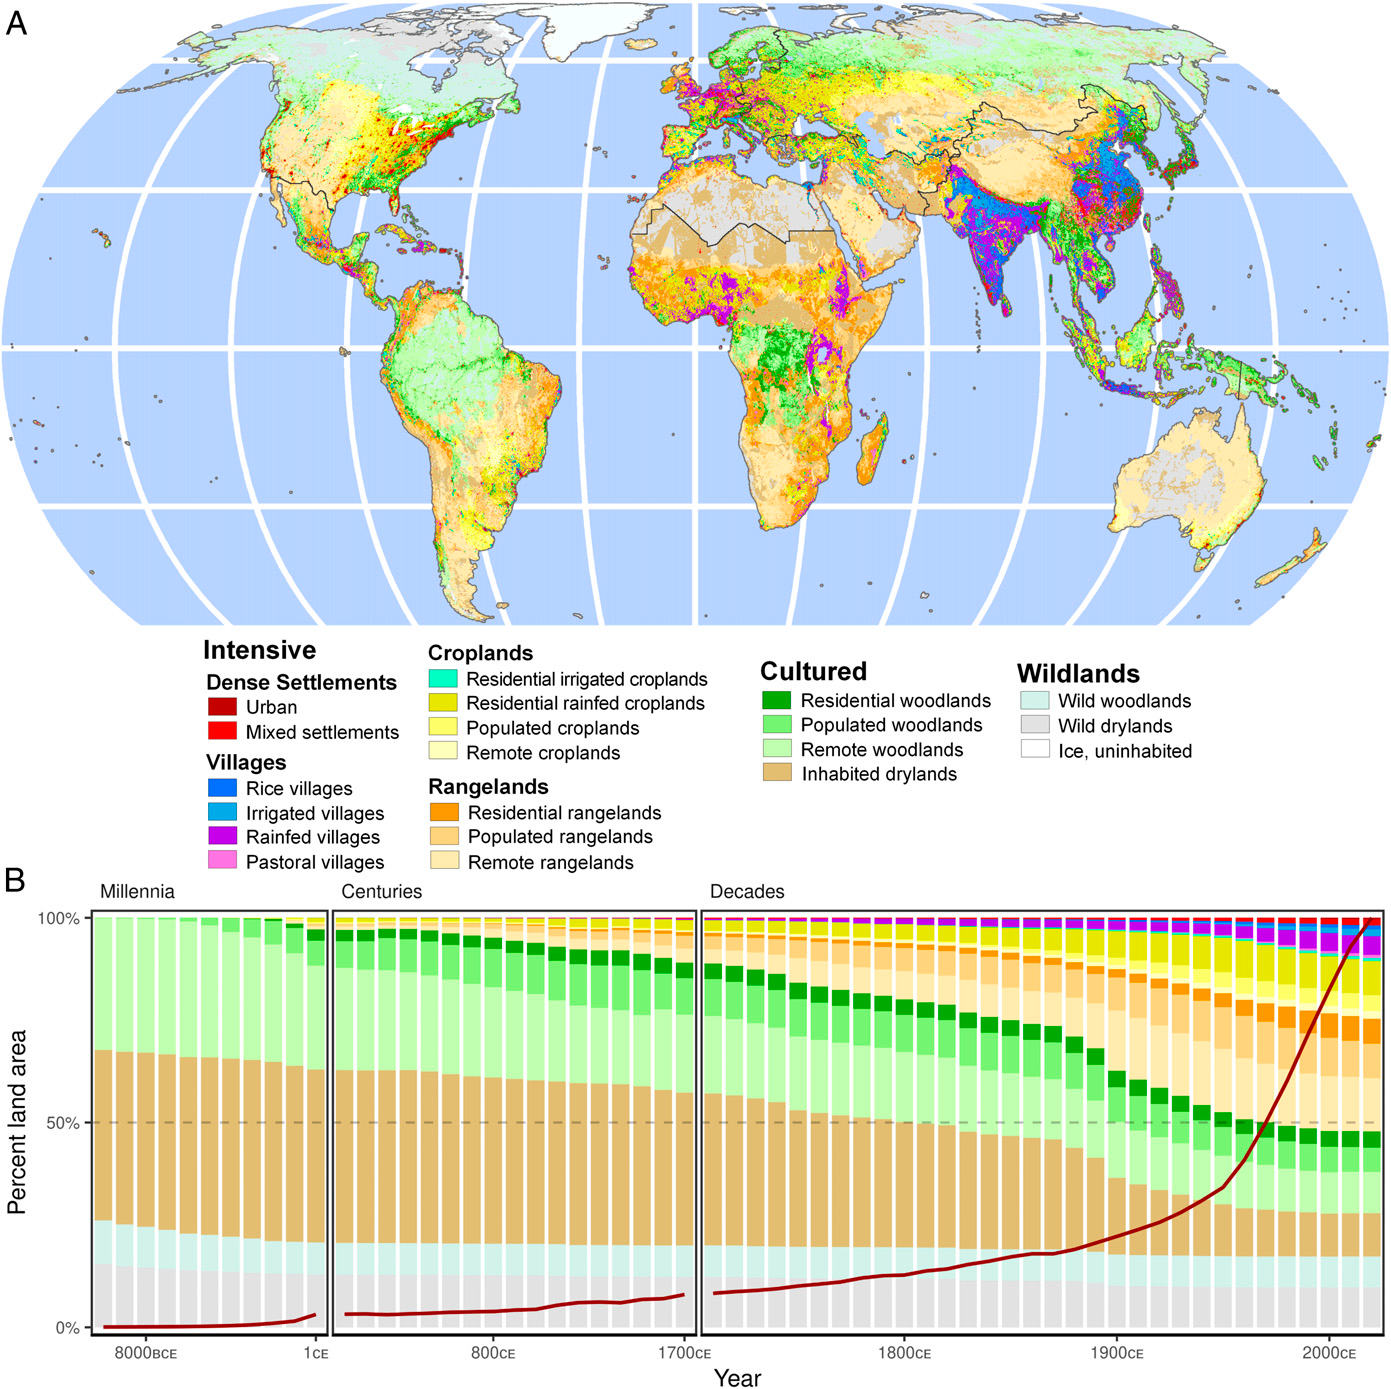
\includegraphics{fig/anthromes.png}

Only about 17\% of Earth's land was without
evidence of prior human habitation or use over the past 12,000 y.
Yet, even this low percentage is certainly an overestimate, based
on growing evidence that the most up-to-date global change models
remain biased toward underestimating the importance of early
human habitation and land use, especially in areas where seasonal
and temporary habitation and use of land predominates

\href{https://www.pnas.org/content/118/17/e2023483118}{Ellis}
\href{pdf/Ellis_2021_Degradation_Loss.pdf}{(pdf)}
\href{Ellis_2021_Degradation_Loss_SI.pdf}{(pdf SI)}

\href{https://en.wikipedia.org/wiki/Anthropogenic_biome}{Wikipedia: Anthromes}

\hypertarget{living-planet-index}{%
\section{Living Planet Index}\label{living-planet-index}}

\emph{Ritchie}

The Living Planet Index is the biodiversity metric that always claims the headlines. Unfortunately many of these headlines are wrong. The index is very easy to misinterpret.

The Living Planet Index reports an average decline of 68\% across tens of thousands of wildlife populations since 1970. This does not tell us anything about the number of individuals, species or populations lost, or even the share of populations that are shrinking.

Before reporting on the Living Planet Index we should understand what it actually tells us about the world's wildlife. We should also be aware of the misconceptions and pitfalls of using this index to capture the changes in more than 20,000 of the world's animal populations.

``In the last 50 years, Earth has lost 68\% of wildlife, all thanks to us humans'' (India Times)

``Humanity has wiped out 60\% of animal populations since 1970, report finds'' (The Guardian)

``We've lost 60\% of wildlife in less than 50 years'' (World Economic Forum)

These are just three of many headlines covering the Living Planet Index. But they are all wrong. They are based on a misunderstanding of what the Living Planet Index shows.

\textbf{What does `average decline' actually mean?}

The Living Planet Index (LPI) measures the average change in the number of individuals across the world's animal populations. A `population' is defined as a species within a geographical area. So, despite being the same species, the African elephant in South Africa and Tanzania are counted as different populations.

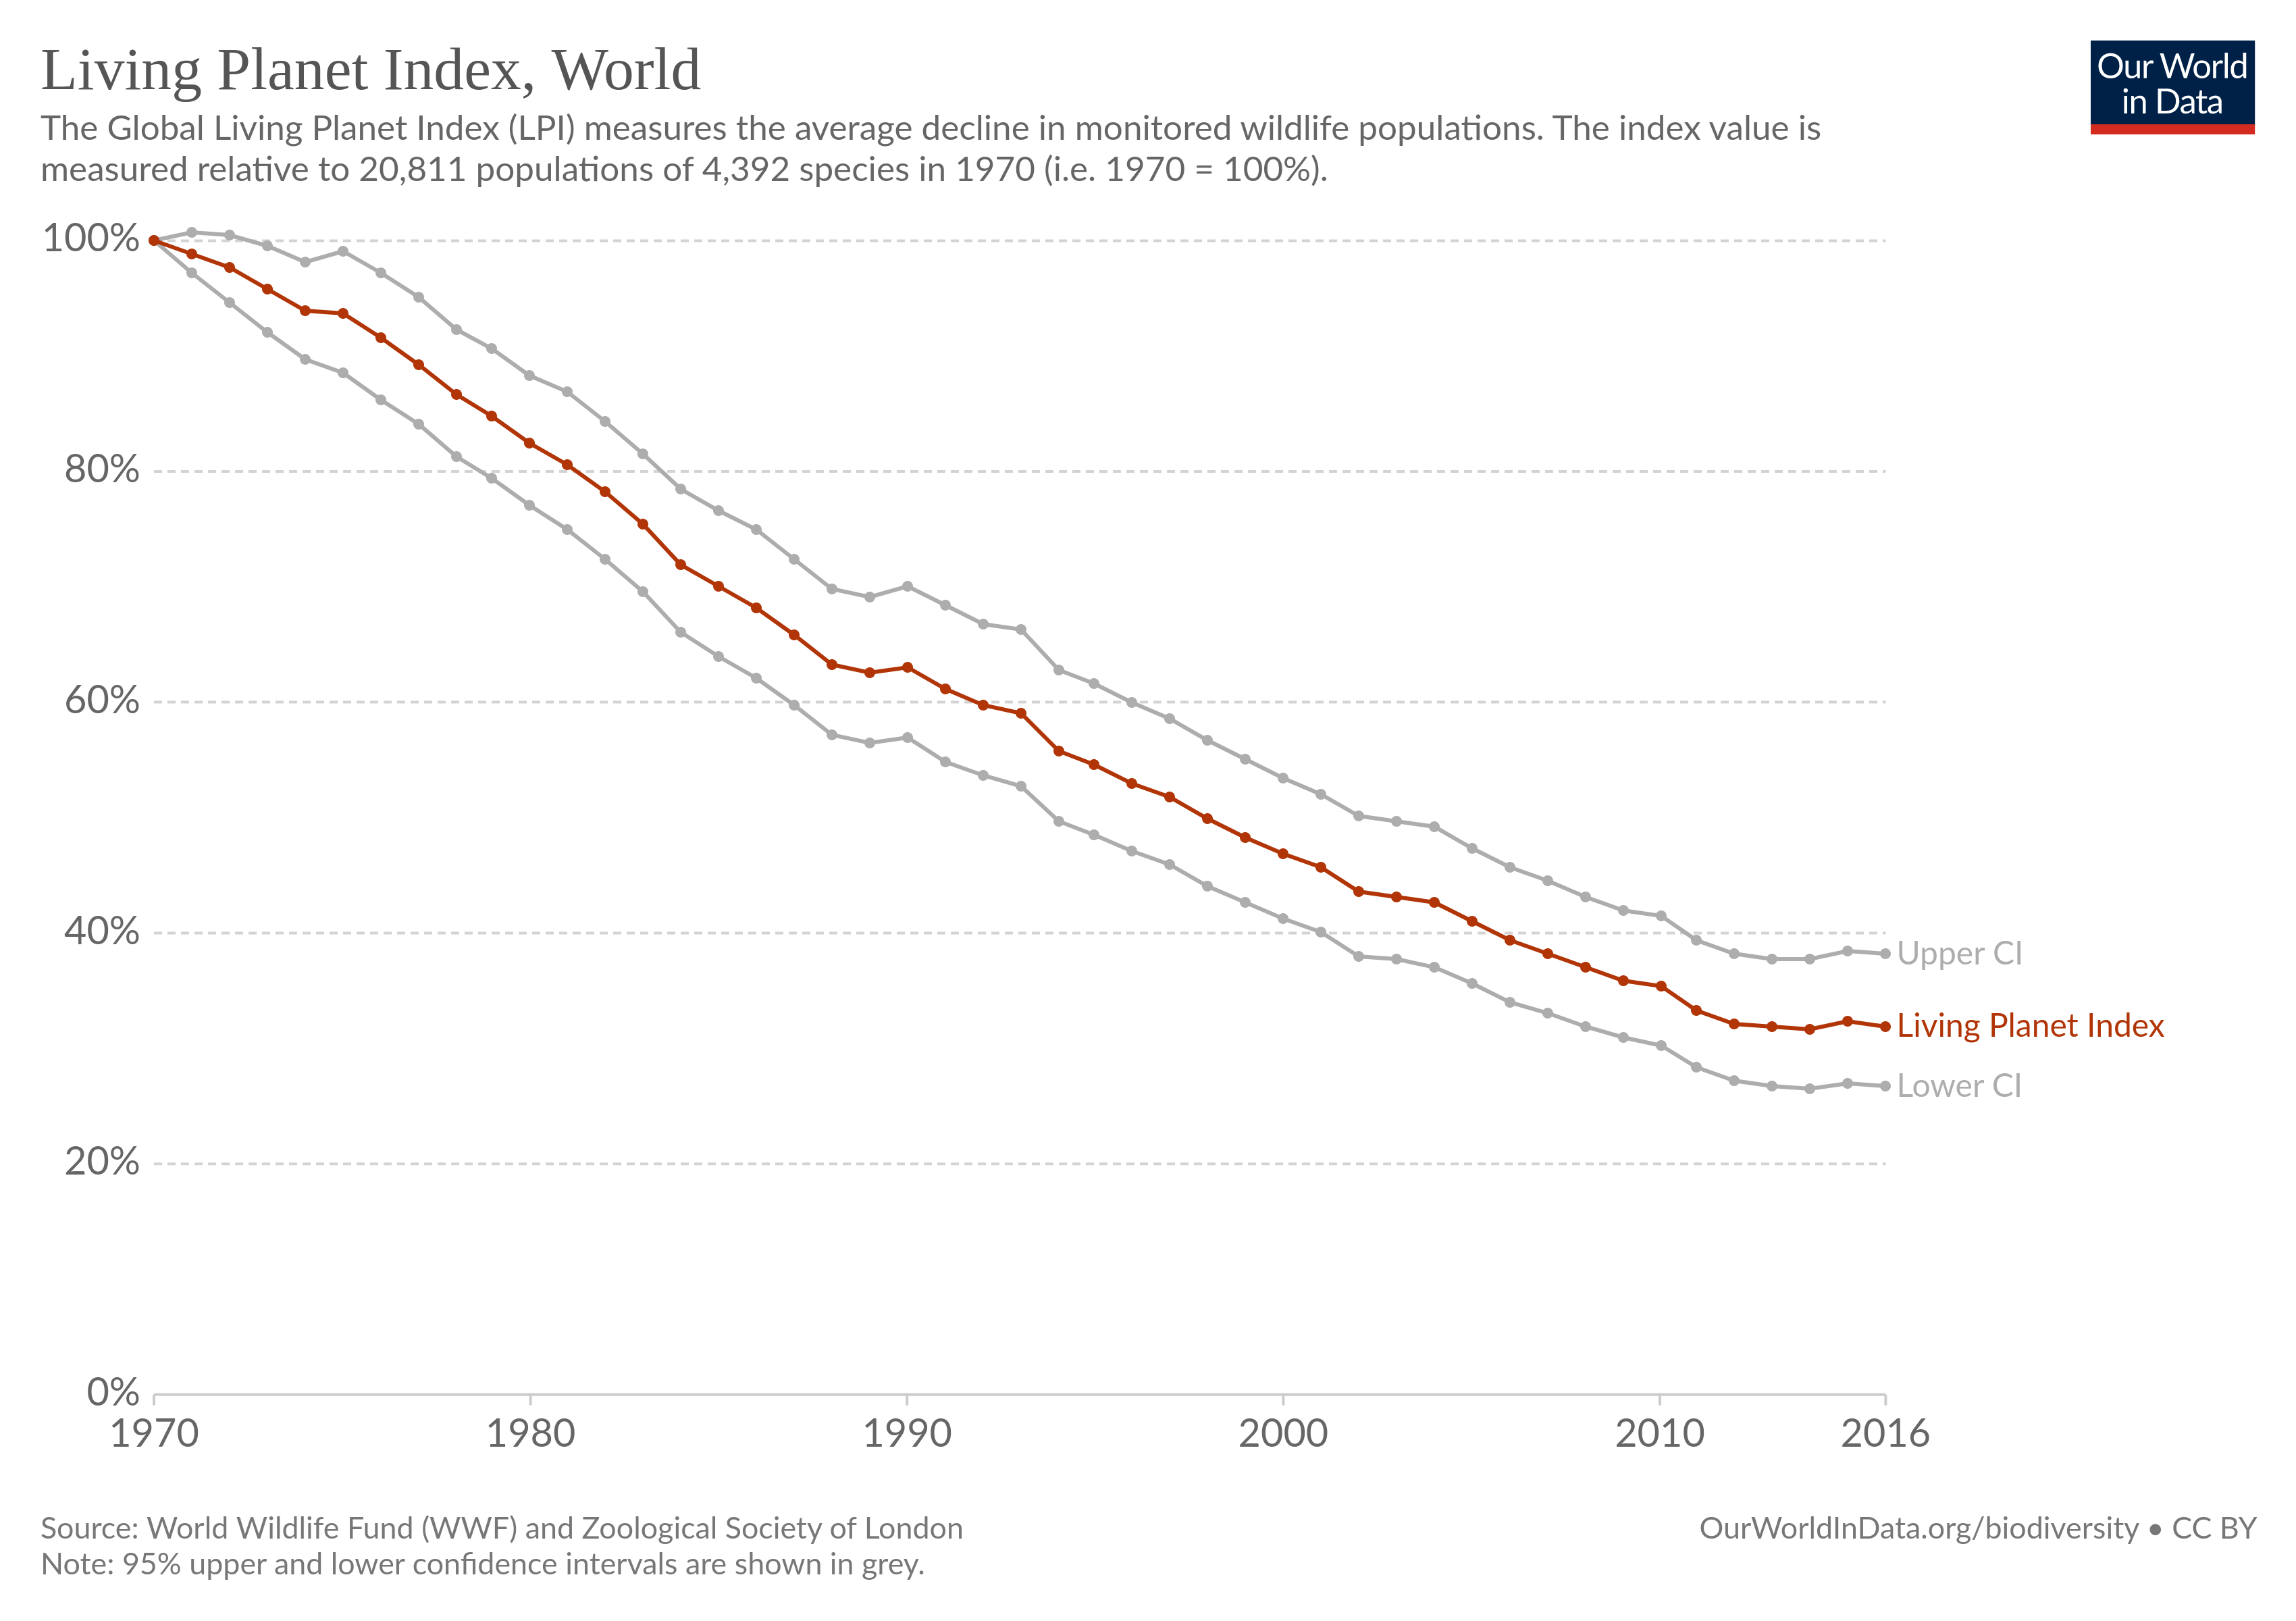
\includegraphics{fig/global-living-planet-index.png}

The Living Planet Index tells us that studied animal populations have seen an average decline of 68\% since 1970

In the latest report it covered 20,811 populations of 4,392 species across the world. It only covers vertebrate species -- mammals, birds, fish, reptiles and amphibians. It includes a large number of populations from each world region, however the tropics tend to be underrepresented relative to Europe and North America. This is not ideal, considering the tropics are home to the greatest diversity of species and is where wildlife is most threatened.

This reveals two further limitations. First, it only covers a tiny percentage of species: Only 15\% of known bird species; 12\% of mammals; 5\% of fish; 4\% of amphibians and merely 2\% of known reptile species. It's hard to say how representative the available data is: it's often the case that the species we are most concerned about (deservedly) get the most attention in the research. Second, many taxonomic groups are not included at all -- nothing on insects, fungi, coral or plants. This is largely due to data availability -- it's easier to count bears than ants.

\href{https://ourworldindata.org/living-planet-index-decline}{Ritchie: OWiD Living Planet Index}

\hypertarget{genetic-manipulation}{%
\chapter{Genetic Manipulation}\label{genetic-manipulation}}

Aedes aegypti makes up about 4\% of the mosquito population in the Keys, a chain of tropical islands off the southern tip of Florida. But it is responsible for practically all mosquito-borne disease transmitted to humans in the region, according to the Florida Keys Mosquito Control District (FKMCD), which is working closely with Oxitec on the project. Researchers and technicians working on the project will release bioengineered male Aedes aegypti mosquitoes, which don't bite, to mate with the wild female population, responsible for biting prey and transmitting disease. The genetically engineered males carry a gene that passes to their offspring and kills female progeny in early larval stages. Male offspring won't die but instead will become carriers of the gene and pass it to future generations. As more females die, the Aedes aegypti population should dwindle.

In late April of this year, project researchers placed boxes containing Oxitec's mosquito eggs at six locations in three areas of the Keys. The first males are expected to emerge within the first two weeks of May. About 12,000 males will exit the boxes each week over the next 12 weeks. In a second phase later this year, intended to collect even more data, nearly 20 million mosquitoes will emerge over a period of about 16 weeks, according to Oxitec.

Genetically engineered mosquitoes are an alternative to insecticides, which are used heavily in the United States to control insect populations. This has resulted in the evolution of mosquitoes that are resistant to insecticides.

\href{https://www.nature.com/articles/d41586-021-01186-6?utm_source=twitter\&utm_medium=social\&utm_content=organic\&utm_campaign=NGMT_USG_JC01_GL_Nature}{Waltz (2021) First genetically modified mosquitoes released in the United States}

\hypertarget{habitat-loss}{%
\chapter{Habitat Loss}\label{habitat-loss}}

\hypertarget{ecosystems}{%
\section{Ecosystems}\label{ecosystems}}

\hypertarget{intact-ecosystems---3}\label{intact-ecosystems---3}}

Just 3\% of the world's land remains ecologically intact with healthy populations of all its original animals and undisturbed habitat.
These fragments of wilderness undamaged by human activities are mainly in parts of the Amazon and Congo tropical forests, east Siberian and northern Canadian forests and tundra, and the Sahara. Invasive alien species including cats, foxes, rabbits, goats and camels have had a major impact on native species in Australia, with the study finding no intact areas left.

The researchers suggest reintroducing a small number of important species to some damaged areas, such as elephants or wolves -- a move that could restore up to 20\% of the world's land to ecological intactness.

Previous analyses have identified wilderness areas based largely on satellite images and estimated that 20-40\% of the Earth's surface is little affected by humans. However, the scientists behind the new study argue that forests, savannah and tundra can appear intact from above but that, on the ground, vital species are missing. Elephants, for example, spread seeds and create important clearings in forests, while wolves can control populations of deer and elk.

The new assessment combines maps of human damage to habitat with maps showing where animals have disappeared from their original ranges or are too few in number to maintain a healthy ecosystem.

It might be possible to increase the ecological intact area back to up to 20\% through the targeted reintroductions of species that have been lost in areas where human impact is still low, provided the threats to their survival can be addressed.

The analysis did not take account of the climate crisis.

\href{https://www.theguardian.com/environment/2021/apr/15/just-3-of-worlds-ecosystems-remain-intact-study-suggests}{Guardian}

Conservation efforts should target the few remaining areas of the world that represent
outstanding examples of ecological integrity and aim to restore ecological integrity to
a much broader area of the world with intact habitat and minimal species loss while
this is still possible.

There have been many assessments of ``intactness'' in recent
years but most of these use measures of anthropogenic impact at a site, rather than
faunal intactness or ecological integrity.

This paper makes the first assessment of faunal
intactness for the global terrestrial land surface and assesses how many ecoregions
have sites that could qualify as Key Biodiversity Areas (KBAs -- sites contributing
significantly to the global persistence of biodiversity) based on their outstanding
ecological integrity (under KBA Criterion C).

Three datasets are combined on species
loss at sites to create a new spatially explicit map of numbers of species extirpated.
Based on this map it is estimated that no more than 2.9\% of the land surface can be
considered to be faunally intact.

The number of ecoregions that
could qualify as Criterion C KBAs could potentially increase land area up to 20\% if
their faunal composition was restored with the reintroduction of 1--5 species.

\href{https://www.frontiersin.org/articles/10.3389/ffgc.2021.626635/full}{Plumptre}
\href{pdf/Plumptre_2021_Ecologically_Intact_Communitiesd.pdf}{(pdf)}

\hypertarget{food-industry-drives-habitat-loss}{%
\section{Food industry drives habitat loss}\label{food-industry-drives-habitat-loss}}

\emph{Memo}

The projected loss of millions of square kilometres of natural ecosystems to meet
future demand for food, animal feed, fibre and bioenergy crops is likely to
massively escalate threats to biodiversity.
Proactive policies targeting how, where, and what food is produced could reduce these threats, with a combination of approaches potentially preventing almost all these losses while contributing to healthier human diets.

The global food system is on course to drive rapid and widespread ecological damage with almost 90\% of land animals likely to lose some of their habitat.
Without fundamental changes, millions of square kilometres of natural habitats could be lost by 2050.

While conventional conservation tactics such as establishing new protected areas
or introducing legislation to save specific species were necessary,
the research underscored the importance of ``reducing the ultimate
stresses to biodiversity -- such as agricultural expansion''.

Shifting to healthier diets would have big benefits in North America, but it is less likely to have a large benefit in regions where meat consumption is low and food insecurity is high.

Responding to the impending biodiversity crisis requires decisions informed by high-resolution,
spatially explicit and species-specific assessments of many thousands of species
to identify the species and landscapes most at risk.
Results from these assessments can be used to help plan appropriate conservation responses,
such as species- or location-specific legislation, and to assess which proactive changes
to food systems have the greatest potential to reduce future threats to biodiversity before
they occur.
The utility of most existing analyses for conservation planning and action has been limited by
coarse spatial resolutions, a focus on a relatively small suite of species or
on generalized biodiversity metrics such as species richness,
or using narrative pathways that are neither tied to current agricultural trajectories
nor able to examine how specific changes to food systems might mitigate future biodiversity declines.

{[}The new research{]} analyse at a high spatial resolution (1.5 × 1.5 km)
the impacts of likely agricultural expansion
on an unprecedented number of species (almost 20,000)
while explicitly accounting for differences in how individual species may be impacted
by agricultural land-use change,
and by analysing how proactive food-system transitions might mitigate future biodiversity decline.

The projected severity of agricultural land-cover change on habitat area means that proactive policies to reduce future demand for agricultural land will probably be required to mitigate widespread biodiversity declines. To investigate the potential of such proactive approaches, we developed a scenario that implemented four changes to food systems: closing crop yield gaps globally, a global transition to healthier diets, halving food loss and waste, and global agricultural land-use planning to avoid competition between food production and habitat protection.

In reality, threats to biodiversity could be considerably greater than those we project: other projections of future agricultural land demand are higher than those we use5, and we do not include the impacts of anthropogenic climate change, habitat fragmentation, over-exploitation, invasive species or pollution5,6,39--41. Climate change is likely to drive widespread changes in biodiversity by altering the location of suitable habitats and environments, and may have synergistic effects with habitat loss and fragmentation from agricultural expansion41. In addition, its effect on agricultural yields42 and the relative suitability of different regions for various crops43 could have indirect impacts on biodiversity by altering patterns of agricultural expansion. Uncertainty in how climatic changes will affect agriculture44 and species45 precludes quantitatively assessing these impacts

\href{https://www.theguardian.com/environment/2020/dec/21/global-food-industry-to-drive-rapid-habitat-loss-research}{Food Industry drives habitat loss (Guardian)}

\href{https://www.nature.com/articles/s41893-020-00656-5.epdf?sharing_token=R2MS-n7EpYm6CQn6PyyqL9RgN0jAjWel9jnR3ZoTv0O6RrkjpmW9fP_y1r0KlZ-Jx6UWX_jcBOXnlP2cYuEslvZu1-m7EgvCszD8mx-fwAIyiIh3Gx1tvRg-Geb5oZYMrgHYywVW7ovXIyZGEpuBr79zSzsD8wwHk_mBt8B8l1kD4xX_vLU2HtS04lrY7S9dTPE2uBW6UFWvOPGd3COAVQjH2qEEkkmbXzsW9f9DQh3JSJxMsDCiFz84VmI_GLPqG-tl6sb70A-DTfHoDYnqvlncEQlHNJLKvMauKaoH-1acinO7dw5-2OW3LzB2QDW-3G7YVVO3x8J2MOFAfUTTGlrNf0ZNDDvSOygvJ1S5z0E6Chteld_Pgugf-yhbLXH9t5TkqNaBYlrrKXb-bgmBYr68yQbKOcBwQy7EfcgOgAnmIVbitCX94Y-_DdD00Vp3YRsOm9AhIG2fmkWzW8OY4nB4Bi2BafrHNNHniHbTJidRx5Uxm8_GFX9tykH3e_M00qDlLJhxMWq1Tl45zu6vdQ\%3D\%3D\&tracking_referrer=www.theguardian.com}{Nature article (shared pdf)}

\href{https://www.nature.com/articles/s41893-020-00656-5}{Nature article (web))}

\hypertarget{mass-extinction}{%
\chapter{Mass Extinction}\label{mass-extinction}}

\emph{Bendell}

The last mass extinction of life on earth, where 95\% of species disappeared,
was due to methane-induced rapid warming of the atmosphere (Lee, 2014; Brand et al, 2016).

\href{pdf/\%20Bendell_2020_Deep_Adaptation.pdf}{Bendell (2018) Deep Adaption: A Map for Navigating Climate Tradegy (pdf)}

\hypertarget{coral-reefs}{%
\section{Coral Reefs}\label{coral-reefs}}

Bad news from the Coral Reefs.
Bleaching is going on and reefs are not healing between events
UNEP is reporting on this issue.

From the 2020 report:

\begin{quote}
Stony corals bleach when warm sea temperatures disrupt the mutualistic relationship between
the algal symbionts, called zooxanthellae, that reside within the host coral tissues (Douglas
2003). Corals can either regain their zooxanthellae (Baker 2001) and survive or die if
temperature stress persists. The third global coral bleaching event, which started in 2014 and
extended well into 2017, was the longest coral bleaching event on record (Eakin et al.~2019).
The length of the event means corals in some parts of the world had no time to recover in 2014,
2015 or 2016 during the cool/winter season, prior to experiencing bleaching the following year.
Van Hooidonk et al.~(2013, 2014, 2016 and 2017) found that a majority of coral reefs are
projected to experience annual severe bleaching (ASB) by the mid-2040's under a business-as-
usual emissions scenario (RCP8.5). This means that the recent global bleaching event of 2014-
2017 represents what climate models suggest may become the norm over the coming few
decades. Lower frequencies of bleaching events per decade (e.g., 2x or 4x per decade) are
projected to occur earlier than ASB. ASB is projected here because annual severe bleaching is a
time beyond which coral reefs seem certain to change (and possibly rapidly degrade).
Importantly though, great spatial variation exists in the projected timing of the onset of ASB
conditions among the world's coral reefs. This variation will be a major driver of differences in
the relative vulnerability of coral reef ecosystems to climate change.
\end{quote}

\begin{quote}
In the IPCC's widely adopted vulnerability assessment framework, vulnerability is a function of
exposure to climate and non-climate threats and sensitivity to these threats, which yields
potential impacts that are moderated by adaptive capacity (Turner et al.~2003). Sensitivity and
adaptive capacity can be collectively seen as resilience (Marshall and Marshall 2007), i.e., the
capacity of a system to absorb or withstand stressors such that the system maintains its
structure and functions in the face of disturbance and change, and the capacity to adapt to
future challenges (McLeod et al.~2019). Managing coral reefs for resilience entails reducing
coral reef vulnerability to climate change by reducing exposure to non-climate threats (i.e., local-
scale anthropogenic stress, Anthony et al.~2014).
\end{quote}

\begin{quote}
A key challenge for reef management lies in deciding where to target actions to reduce
anthropogenic stress, ensuring efficacy as well as cost effectiveness of actions taken.
Ecosystem and Resilience Based Management (EBM and RBM) are becoming increasingly
sophisticated (Mills et al.~2015, McLeod et al.~2019), and software that combines and analyzes
spatial data is increasingly accessible and used in planning to strike a balance between what
can be competing conservation and development objectives (Watts et al.~2009). For example,
protecting biodiversity, providing for sustainable fisheries, and minimizing user conflicts are
among the highest priorities during marine spatial planning (MSP) efforts in reef areas (Agardy
et al.~2011). Incorporating spatial variation in coral reef vulnerability to climate change is
frequently discussed during MSP but, as yet, is rarely operationalized (Anthony et al.~2014). This
will require assessing spatial variation in the key vulnerability components -- exposure and
resilience - at a locally relevant scale (one km to 10s of km).
\end{quote}

\href{https://www.unenvironment.org/resources/report/coral-bleaching-futures}{UNEP Coral Bleaching Futures 2017}
\href{/pdf/UNEP_2017_Coral_Bleaching_Futures.pdf}{(pdf)}

\href{https://www.unenvironment.org/resources/report/projections-future-coral-bleaching-conditions-using-ipcc-cmip6-models-climate}{UNEP Coral Reefs Report 2020}
\href{/pdf/UNEP_2020_Coral_Reefs_CMIP6.pdf}{(pdf)}

\href{https://www.cell.com/trends/ecology-evolution/fulltext/S0169-5347(20)30306-2\#secst0025}{Biological Conservation Issues 2021 Scanning}

\hypertarget{extinction-rate}{%
\section{Extinction Rate}\label{extinction-rate}}

\hypertarget{compared-to-5th-mass-extinction}{%
\subsection{Compared to 5th Mass Extinction}\label{compared-to-5th-mass-extinction}}

\emph{Neubauer Abstract}

The Cretaceous--Paleogene mass extinction event 66 million years ago eradicated three quarters of marine and terrestrial species globally. However, previous studies based on vertebrates suggest that freshwater biota were much less affected. Here we assemble a time series of European freshwater gastropod species occurrences and inferred extinction rates covering the past 200 million years. We find that extinction rates increased by more than one order of magnitude during the Cretaceous--Paleogene mass extinction, which resulted in the extinction of 92.5\% of all species. The extinction phase lasted 5.4 million years and was followed by a recovery period of 6.9 million years. However, present extinction rates in European freshwater gastropods are three orders of magnitude higher than even these revised estimates for the Cretaceous--Paleogene mass extinction. Our results indicate that, unless substantial conservation effort is directed to freshwater ecosystems, the present extinction crisis will have a severe impact to freshwater biota for millions of years to come.

\href{https://www.nature.com/articles/s43247-021-00167-x}{Neubauser (2021) Current extinction rate in European freshwater gastropods greatly exceeds that of the late Cretaceous mass extinction}

\href{https://www.naturetoday.com/intl/en/nature-reports/message/?msg=27702\&utm_source=rssfeed\&utm_medium=rss\&utm_campaign=web-rss-nb}{Nature Today (2021) Biodiversity devastation: human-driven decline requires millions of years of recovery}

\href{https://www.independent.co.uk/independentpremium/mass-extinction-humans-dinosaurs-biodiversity-b1853021.html}{Independent (2021) Human-driven biodiversity loss faster than mass extinction when dinosaurs were wiped out}

\hypertarget{material-extraction}{%
\chapter{Material Extraction}\label{material-extraction}}

\hypertarget{material-and-energy-productivity}{%
\section{Material and Energy Productivity}\label{material-and-energy-productivity}}

\emph{Steinberger Abstract}

Resource productivity, measured as GDP output per resource input, is a widespread sustainability indicator
combining economic and environmental information. Resource productivity is ubiquitous, from the IPAT identity to the analysis of
dematerialization trends and policy goals. High resource productivity is interpreted as the sign of a resource-efficient, and hence
more sustainable, economy. Its inverse, resource intensity (resource per GDP) has the reverse behavior, with higher values
indicating environmentally inefficient economies. In this study, we investigate the global systematic relationship between material,
energy and carbon productivities, and economic activity. We demonstrate that different types of materials and energy exhibit
fundamentally different behaviors, depending on their international income elasticities of consumption. Biomass is completely
inelastic, whereas fossil fuels tend to scale proportionally with income. Total materials or energy, as aggregates, have intermediate
behavior, depending on the share of fossil fuels and other elastic resources. We show that a small inelastic share is sufficient for the
total resource productivity to be significantly correlated with income. Our analysis calls into question the interpretation of resource
productivity as a sustainability indicator. We conclude with suggestions for potential alternatives.

\href{https://pubs.acs.org/doi/10.1021/es1028537\#}{Steinberger (2011)}
\href{pdf/Steinberger_2011_Material_and_Energy_Productivity.pdf}{(pdf)}

\hypertarget{physical-economy-of-united-states}{%
\section{Physical Economy of United States}\label{physical-economy-of-united-states}}

\emph{Gierlinger}

This article explores the long-term historical development of
the physical economy of the United States and the evolution
of its industrial metabolism.

\textbf{No dematerialization}

The United States is not only the world's largest economy, but it is also one of the world's
largest consumers of natural resources. The country, which is inhabited by some 5\% of the
world's population, uses roughly one-fifth of the global primary energy supply and 15\% of
all extracted materials. This article explores long-term trends and patterns of material use
in the United States. Based on a material flow account (MFA) that is fully consistent with
current standards of economy-wide MFAs and covers domestic extraction, imports, and
exports of materials for a 135-year period, we investigated the evolution of the U.S. industrial
metabolism. This process was characterized by an 18-fold increase in material consumption,
a multiplication of material use per capita, and a shift from renewable biomass toward
mineral and fossil resources. In spite of considerable improvements in material intensity, no
dematerialization has happened so far; in contrast to other high-income countries, material
use has not stabilized since the 1970s, but has continued to grow. This article compares
patterns and trends of material use in the United States with those in Japan and the United
Kingdom and discusses the factors underlying the disproportionately high level of U.S. per
capita resource consumption.

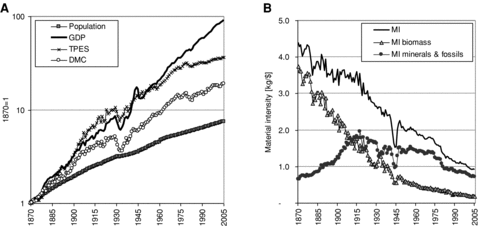
\includegraphics{fig/material_use_US.png}

\emph{Figure: Material use and economic development in the United States:
(a) development of population, gross domestic product (GDP),domestic material consumption (DMC),
and total primary energy supply (TPES); and
(b) material intensity (MI) in kilograms per unit GDP.
MI is defined as DMC/GDP.
Note the logarithmic scale}

\href{https://onlinelibrary.wiley.com/doi/full/10.1111/j.1530-9290.2011.00404.x}{Gierlinger (2011) Physical Economy of United States}
\href{pdf/Gierlinger_2011_Physical_Economy_of_US.pdf}{(pdf)}

\hypertarget{mining}{%
\section{Mining}\label{mining}}

\hypertarget{battery-metals}{%
\subsection{Battery Metals}\label{battery-metals}}

\emph{Beslik}

Rare earth metals are at the core of every major technology today. Smartphones, laptops, wind turbines, electric cars, and medical devices, you name it.

They're also widely used in defence technology like jets and guided missile systems. Rare earth metals are essential to modern technology.

It's important to distinguish between: `rare-', `precious-', and `critical-' earth elements. The terms are not interchangeable, but unfortunately often are in popular media.

It's also important to distinguish between `reserves' and `resources'. Reserves denote the amount that can be technically recovered at a cost that is financially feasible at the present price. Resources include all that can be technically recovered at any price.

Electric vehicles typically use two precious earth metals: gold and silver. These are used in minute quantities in the circuit boards, which also occurs in modern fossil fuelled vehicles. The circuit boards run the electronics. These valuable metals are fully recyclable.

Critical earth elements typically found in EV batteries are: lithium and cobalt, both fully recyclable. Both Lithium and cobalt metals can be reused over and over repeatedly. These two elements are not particularly rare -- cobalt can be found in most rocks, and lithium is the first metal in the periodic table and one of only three elements created in the primordial Big Bang. Lithium is the 32nd most common element on our planet.

But both metals are critical because of modern societies' dependence on lithium-ion battery technology for mobile phones, laptops, and now EVs. And also, in the case of cobalt, because of geopolitics: the bulk of the cobalt supply comes from the politically unstable Democratic Republic of Congo. While there are plenty of lithium and cobalt resources, there are fewer reserves of them. Cobalt is a by-product of nickel and copper mines, and is therefore dependent on the economic viability of those mining operations.

Worldwide sources of lithium are broken down by ore-deposit type as follows: closed-basin brines, 58\%; pegmatites and related granites, 26\%; lithium-enriched clays, 7\%; oilfield brines, 3\%; geothermal brines, 3\%; and lithium-enriched zeolites, 3\% (2013 statistics USGS). Of those, closed basin brines are the most important source of lithium reserves.

Put simplistically, dissolved lithium salts are most commonly mined by drilling down to underground saline deposits and pumping the saline to the surface where it is left to dry in the desert sun, before being processed into lithium metal (and other elements, like potash and magnesium).

China currently holds a near monopoly on supply. China mines 94-97\% of the rare earth metals globally and, while efforts have increased in America and Europe to find alternative supplies, there are still no clear avenues to diversifying supply. China has become the world's largest producer simply because Western nations don't want to do the dirty work that is required to produce rare earths.

The reason most often cited for this shift to China is cheap labour. However another, which is often tacitly acknowledged, is lack of environmental regulation. This has meant that costs associated with proper environmental protection -- required if manufacturing occurred in the west -- have not been built in to the price of goods.

Australia has substantial rare element deposits. However, the current major Australia processing operation involves a site in Malaysia. This controversial project by Lynas has sparked a major local environmental protest campaign led by Malay residents concerned about environmental and health impacts.

Rare earth metals are currently extracted through mining, which comes with a number of downsides. First, it's costly and inefficient because extracting even a very small amount of rare earth metals requires large areas to be mined. Second, the process can have enormous environmental impacts. Mining for rare earth minerals generates large volumes of toxic and radioactive material, due to the co-extraction of thorium and uranium, radioactive metals which cause problems for the environment and human health.

These are the \href{https://www.mining.com/web/ranked-top-25-nations-producing-battery-metals-for-the-ev-supply-chain/}{locations} where the mining of battery metals is taking place.

\href{https://esgonasunday.substack.com/p/week-51-merry-electric-christmas}{Beslik (2021) Merry Electric Christmas}

\hypertarget{pollution}{%
\chapter{Pollution}\label{pollution}}

\hypertarget{fertility}{%
\section{Fertility}\label{fertility}}

Following current projections, the median sperm count is set to reach zero in 2045.

\href{https://www.theguardian.com/us-news/2021/feb/26/falling-sperm-counts-human-survival}{The Guardian}

\emph{Asexuality}

Asexuality, an orientation estimated to apply to 1\% of the global population,
although some think the number is higher.

``Our society is increasingly hyper-sexualised,'' she says, ``and that can make it particularly alienating for asexual people who don't have those feelings, or don't want to live that life.''

Asexuality has sometimes been dubbed the ``forgotten'' or ``invisible'' orientation owing to its lack of public prominence. Until recently it was deemed a medical issue by the US's Diagnostic and Statistical Manual of Mental Disorders -- which added an exception in 2013 to state that asexuals do not have a desire disorder -- and many continue to erroneously dismiss it as an affliction.

It has also been labelled ``the world's first internet orientation,'' implying that people who feel this way have only existed since the advent of the internet -- and suggesting it's a fad.

\href{https://www.theguardian.com/lifeandstyle/2021/mar/21/i-dont-want-sex-with-anyone-the-growing-asexuality-movement}{Guardian}

\hypertarget{plastics}{%
\section{Plastics}\label{plastics}}

\textbf{Extended Producer Responsibility (EPR)}

\emph{Independent}

The United States recycles less than 9 per cent of items
but ``the plastics industry has managed to convince us all that it's our fault''.

Plastic production is booming with more than half of all plastic ever made
created within the last two decades.

Vast amounts of plastic aren't recycled for reasons including its complex mix of resins;
contamination or difficulty in sorting; or the simple fact it's cheaper to make virgin plastic.

The pollution ends up in landfill, is incinerated or shipped overseas to less wealthy nations.

An estimated 10 million tons of plastic ends up in the ocean annually -
the equivalent of a garbage truck every minute.

Despite spending millions of dollars in ad campaigns that highlighted consumers' responsibility for recycling, the plastics industry was aware that large-scale recycling would not work.

The recycling movement is ``often bankrolled by companies that wanted to drill home
the message that it is your responsibility
to deal with the environmental impact of their products.

The ``real behaviour change'' has to come from those who make the plastic in the first place.
Legislation called ``extended producer responsibility (EPR)''
would shift more obligation to industry for the environmental price-tag of their products.

\href{https://www.independent.co.uk/climate-change/news/john-oliver-plastics-recycling-b1820614.html}{Independent}

\hypertarget{dirty-thirty}{%
\subsection{Dirty-Thirty}\label{dirty-thirty}}

\emph{Thoumi}

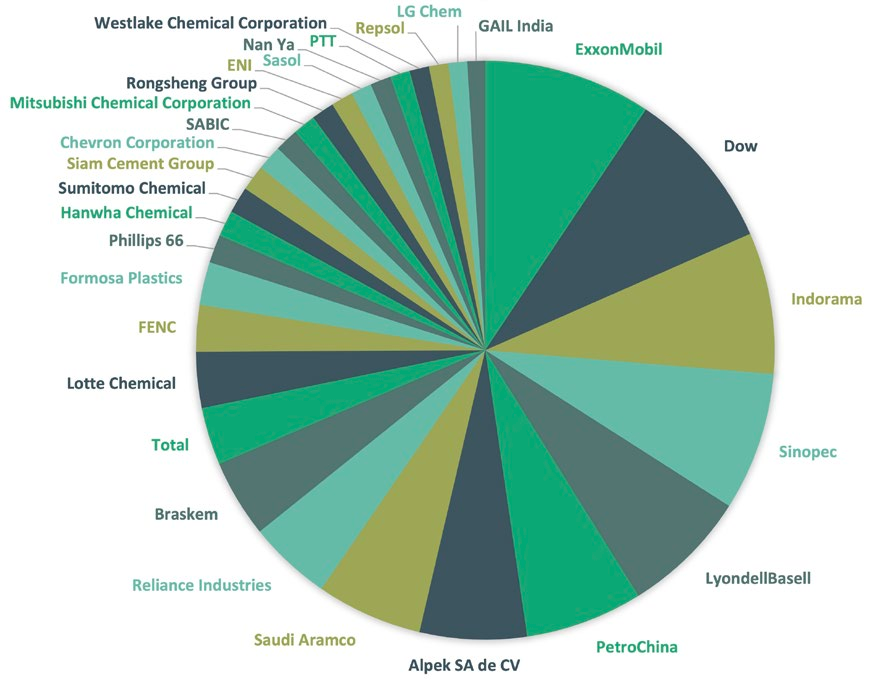
\includegraphics{fig/Dirty-Thirty.png}

• In 2019, 30 publicly traded companies - the Dirty Thirty - produced
58\% of single-use plastic (SUP) 1 . The top 10 - ExxonMobil, Dow, Indorama,
Sinopec, LyondellBasell, PetroChina, Alpek, Aramco, Reliance and Braskem -
were responsible for 39\%.
• The Dirty Thirty footprint is highly concentrated in a few clusters, including
the US Plastic Production Corridor and the EU Trilateral Chemical Region.
• The top ten equity and top ten fixed income investors own 76\% and 43\%
of the Dirty Thirty's equity and debt respectively. BlackRock, Vanguard
and Capital Group are on both lists.
• The Dirty Thirty's SUP supply chain encompasses multiple risk factors ranging
from carbon and other emissions, end-product waste and operational spills.
The industry poses threats to society and human health, with amplified
effects often felt by more marginalised or vulnerable communities.
• As a result of its wide-ranging impact, the industry is more exposed
than others to regulation, policy change and legal challenges. The Dirty
Thirty in particular are experiencing increasing pressure from business
clients to meet 2025 SUP reduction commitments, increasingly viewed as
accountable for combatting plastic pollution.
• Plastic pollution is forecast to triple by 2040, with 80\% expected to come
i
from SUP. Without serious change, by 2050, in a 1.5°C scenario, plastic
lifecycle emissions are forecast to make up roughly 13\% of carbon budgets. ii
• Solving the plastic pollution crisis, including the pollution from plastic
production itself - for example, GhG emissions and toxic chemical releases
- will play a key role in addressing the climate crisis and achieving goals
outlined in the Paris Agreement.
• Both solutions and green financing are available for companies looking to
retool towards sustainable plastic production, but uptake is slow among the
Dirty Thirty, many of whom appear to be adopting a wait-and-see approach.

\href{pdf/Dirty-Thirty.pdf}{Thoumi (2021) Dirty-Thirty (pdf)}

\hypertarget{virgin-polymer-production}{%
\subsection{Virgin Polymer Production}\label{virgin-polymer-production}}

\emph{Guardian}

Twenty companies are responsible for producing more than half of all the single-use plastic waste in the world, fuelling the climate crisis and creating an environmental catastrophe, new research reveals.

Among the global businesses responsible for 55\% of the world's plastic packaging waste are both state-owned and multinational corporations, including oil and gas giants and chemical companies, according to a comprehensive new analysis.

The Plastic Waste Makers index reveals for the first time the companies who produce the polymers that become throwaway plastic items, from face masks to plastic bags and bottles, which at the end of their short life pollute the oceans or are burned or thrown into landfill.

The enormous plastic waste footprint of the top 20 global companies amounts to more than half of the 130m metric tonnes of single-use plastic thrown away in 2019, the analysis says.

\href{https://www.theguardian.com/environment/2021/may/18/twenty-firms-produce-55-of-worlds-plastic-waste-report-reveals}{Guardian}

\emph{Mindero Foundation}

\begin{quote}
The Minderoo Foundation is funded in part by one of the world's largest suppliers of iron ore.
The plastics industry has been allowed to operate with minimal regulation and transparency for decades. Government policies, where they exist, tend to focus on the vast number of companies that sell finished plastic products. Relatively little attention has been paid to the smaller number of businesses at the base of the supply chain that make ``polymers'' -- the building blocks of all plastics -- almost exclusively from fossil fuels.
\end{quote}

These companies are the source of the single-use plastic crisis: their production of new ``virgin'' polymers from oil, gas and coal feedstocks perpetuates the take-make-waste dynamic of the plastics economy. The economies of scale for fossil-fuel-based production are undermining transition to a ``circular'' plastic economy, with negative impacts on waste collection rates, on end-of-life management and on rates of plastic pollution. The focus needs to be on producing recycled polymers from plastic waste, on re-use models and on alternative substitute materials.

\begin{verbatim}
1. In 2019, just 20 polymer producers accounted for more than half of all single-use plastic waste generated globally – and the top 100 accounted for 90 per cent.  
2. Major global investors and banks are enabling the single-use plastics crisis.  
3. There has been a collective industry failure to transition away from fossil-fuel-based feedstocks.  
4. Planned expansion of virgin polymer production capacity threatens to overwhelm hopes of a circular plastics economy.  
5. Single-use plastic waste is an entrenched geopolitical problem.  
\end{verbatim}

\href{https://sourceofplasticwaste.org/}{Media Story}

\href{https://www.minderoo.org/plastic-waste-makers-index/findings/executive-summary/}{Mindero Foundation: Plastic Waste Makers Index}

\emph{American Chemistry Council}

\textbf{Minderoo Report Fails To Factor In Plastics' Key Role In Lowering Greenhouse Gas Emissions.}

The Minderoo Foundation misconstrues the relationship between plastics and our carbon footprint. Some of the most comprehensive studies to date have found that replacing plastics with other materials would drive up waste and carbon impacts.

Glaringly absent from the Minderoo report is a recognition of plastic's critical role in enabling innovations we need for sustainable infrastructure, such as solar panels, wind turbines, and electric vehicles and charging stations.

\href{https://www.prnewswire.com/news-releases/misleading-minderoo-report-fails-to-factor-in-plastics-key-role-in-lowering-greenhouse-gas-emissions-301293161.html}{American Chemistry Council}

\hypertarget{nurdles}{%
\subsection{Nurdles}\label{nurdles}}

\emph{McVeigh}

Nurdles, the colloquial term for ``pre-production plastic pellets'', are the little-known building block for all our plastic products. The tiny beads can be made of polyethylene, polypropylene, polystyrene, polyvinyl chloride and other plastics. Released into the environment from plastic plants or when shipped around the world as raw material to factories, they will sink or float, depending on the density of the pellets and if they are in freshwater or saltwater.

They are often mistaken for food by seabirds, fish and other wildlife. In the environment, they fragment into nanoparticles whose hazards are more complex. They are the second-largest source of micropollutants in the ocean, by weight, after tyre dust. An astounding 230,000 tonnes of nurdles end up in oceans every year.

Like crude oil, nurdles are highly persistent pollutants, and will continue to circulate in ocean currents and wash ashore for decades. They are also ``toxic sponges'', which attract chemical toxins and other pollutants on to their surfaces.

``The pellets themselves are a mixture of chemicals -- they are fossil fuels,'' says Tom Gammage, at the Environmental Investigation Agency (EIA), an international campaign group. ``But they act as toxic sponges. A lot of toxic chemicals -- which in the case of Sri Lanka are already in the water -- are hydrophobic {[}repel water{]}, so they gather on the surface of microplastics.

``Pollutants can be a million times more concentrated on the surface of pellets than in the water,'' he says. ``And we know from lab studies that when a fish eats a pellet, some of those pollutants come loose.''

Nurdles also act as ``rafts'' for harmful bacteria such as E coli or even cholera, one study found, transporting them from sewage outfalls and agricultural runoff to bathing waters and shellfish beds. The phenomenon of ``plastic rafting'' is increasing.
Advertisement

Yet nurdles, unlike substances such as kerosene, diesel and petrol, are not deemed hazardous under the International Maritime Organization's (IMO's) dangerous goods code for safe handling and storage. This is despite the threat to the environment from plastic pellets being known about for three decades, as detailed in a 1993 report from the US government's Environmental Protection Agency on how the plastics industry could reduce spillages.

McVeigh (Guardian) (2021) Nurdles: the worst toxic waste you've probably never heard of{]}(\url{https://www.theguardian.com/environment/2021/nov/29/nurdles-plastic-pellets-environmental-ocean-spills-toxic-waste-not-classified-hazardous})

\hypertarget{finance}{%
\subsection{Finance}\label{finance}}

\emph{Memo}

To address plastic pollution, a fundamental shift
away from business models that depend on sin-
gle-use packaging towards those that prioritise
reuse and more localized supply chains and services
is needed.
Banks should make funding of corporate
actors within the plastic packaging supply
chain contingent on companies implement-
ing best practice.
Governments should stop protecting banks
and re-write the rules of finance to hold
banks liable for the damage caused by their
lending.
Companies must adopt international best
practice to reduce the production and use
of virgin plastic and increase the reusability
of plastic packaging products.

Banks are silent and out of touch
with reality
This global public outcry led to a set of govern-
ment and business responses. As of June 2020, it
was reported that 69 countries had passed a full or
partial ban on plastic bags. Some companies have
made comparatively strong commitments to reduce
plastic packaging. Despite public outcry over the serious impacts
of plastic pollution, and efforts by some companies
within the plastic value chain to reduce their impacts,
none of the banks analysed have developed due
diligence systems, contingent loan criteria or financ-
ing exclusions when it comes to this industry. This
means banks are currently not taking responsibility
to understand, measure, and reduce the impacts of
their loans within the plastics value chain.
By indiscriminately funding actors in the plastic
supply chain, banks have failed to acknowledge
their role in enabling global plastic pollution. They
have fallen far behind the crowd of other actors that
contribute to the plastic pollution crisis.

By indiscriminately funding actors in the plastic
supply chain, banks have failed to acknowledge
their role in enabling global plastic pollution.
They have fallen far behind other actors that
contribute to the plastic pollution crisis.

The concentration of finance
from banks Headquarted in
a few jurisdictions indicates
that legislative measures, such
as introducing lender liability
which holds financiers and
investors responsible for the
impacts their financing has on
biodiversity, could be highly
impactful even when initially
implemented in a small number
of geographic regions.

A limited number of banks have started to adopt
policies that allow them to limit investments for other
high biodiversity impacting sectors such as fossil
fuels, forest products, and some agricultural commod-
ities. However, this has not yet occurred for plastics.

Governments and financial institutions
should both recognise that investment in the plastics
supply chain without sufficient investment in the
plastics value recovery chain (reduction, recovery,
re-use and recycling), causes and contributes to this
harm. To remedy the problem, governments should:

Extend investor liability for any future envi-
ronmental or health related legal challenges
to those responsible for plastic pollution,
especially effects of it entering the food
chain.

Introduce a mandatory tax on virgin plastic
at the point of importation to or production
within a country, in order to raise its price
relative to recycled plastics, achieving
equivalence by channeling the receipts from
the tax into incentives to recover and reuse
plastics waste streams. This would require
trade related controls to ensure equivalence
in imported packaging.

Invest in a new generation of recycled
plastics markets by establishing forward
contracting arrangements akin to renew-
able energy feed in tariffs to incentivise
investment in modern recycled plastics
value chains.

\href{https://portfolio.earth/campaigns/bankrolling-plastics/}{Portfolio.earth Bankrolling Plastics}

\hypertarget{chemicals}{%
\section{Chemicals}\label{chemicals}}

\hypertarget{chemicals-pollution}{%
\subsection{Chemicals' Pollution}\label{chemicals-pollution}}

\begin{quote}
The chemicals industry consumes more than 10\% of fossil fuels produced globally and emits an estimated 3.3 gigatons of greenhouse gas emissions a year, more than India's annual emissions.
\end{quote}

While the industry has an important role to play in moving to low-carbon economies -- providing coatings for solar panels, lightweight plastics to reduce vehicles' energy consumption and insulating materials for buildings -- it's also hugely carbon intensive and predicted to become more so.

Oil companies have been betting on chemicals as a way to remain profitable as the world pledges to turn away from fossil fuel energy. The International Energy Agency predicted that petrochemicals could account for 60\% of oil demand in the next decade.

The chemicals sector is the largest industrial user of oil and gas but it has the third-largest carbon footprint -- behind steel and cement -- because only about half of the fossil fuels that the industry consumes are burned for their energy. The rest is used as feedstock for products such as plastics with the emissions released only when these products reach the end of their lives, for example, when waste plastic packaging or an old mattress is incinerated.

Most of the industry's direct carbon dioxide emissions come from burning fossil fuels to power chemical transformations, many of which take place at high temperatures and pressures.

Chemists continue to look for ways to power traditionally heat-driven chemical transformations with electricity instead -- such as the process of converting nitrogen to ammonia, mostly used for fertilizer, which requires temperatures of about 500C (932F).

Many chemical products themselves cannot be decarbonized because they are made of carbon.

Removing fossil fuels from the raw materials used to create carbon-based chemicals and materials is crucial. Products made from fossil fuels -- such as clothes, toys and paints -- is a carbon debt, because the carbon embedded within them will only be emitted in the future.

To stop adding to this debt, chemicals and materials could be made with sources of carbon that are already above ground, such as plants. Bioplastics -- made with plant materials such as sugar, corn or seaweed -- are booming.

Another idea is to turn waste products into raw materials for the chemical industry. Chemists have been using agricultural waste or waste plastics -- even the ultimate waste material, carbon dioxide -- as feedstocks. A Berlin-based startup, Made of Air, is attempting to create plastics from wood waste, while an Icelandic company, Carbon Recycling International, turns captured carbon dioxide emissions into methanol, used in fuels and for making other chemicals such as formaldehyde.

But all these ideas -- especially those involving a shift in feedstocks -- are very hard to implement.

Technologies to turn agricultural or plastic waste into new chemicals are still unproven on a large scale and using carbon dioxide as a raw material will require vast amounts of zero-carbon energy.

Manufacturers making products with plants rather than fossil fuels need to ensure that they do not create new problems through deforestation, destroying wildlife habitat, raising food prices or increasing the use of water or pesticides. Biomass resources also tend to be more spread out, whereas traditionally, chemical plants stay close to where fossil fuel resources are easily accessible.

The clean power infrastructure requirements alone are tremendous. Electrifying Europe's chemicals sector would require 4,900 terawatts of renewable electricity - almost double the total amount of electricity Europe generated in 2019.

One important, but neglected, lever for cutting emissions from the chemical sector is to simply use and produce fewer chemicals.

The business model is driven by how many chemicals you sell, it's not necessarily driven by the added societal value of the chemical.

\href{https://www.theguardian.com/environment/2021/nov/22/chemicals-industry-pollution-emissions-climate}{Guardian (2021) How the chemicals industry's pollution slipped under the radar}

\hypertarget{pfas---forever-chemicals}{%
\subsection{PFAS - ``forever chemicals''*}\label{pfas---forever-chemicals}}

The end of humankind? It may be coming sooner than we think, thanks to hormone-disrupting chemicals that are decimating fertility at an alarming rate around the globe. A new book called Countdown, by Shanna Swan, an environmental and reproductive epidemiologist at Icahn School of Medicine at Mount Sinai in New York, finds that sperm counts have \href{https://www.theguardian.com/us-news/2021/feb/26/falling-sperm-counts-human-survival}{dropped almost 60\% since 1973}. Following the trajectory we are on, Swan's research suggests sperm counts could reach zero by 2045. Zero. Let that sink in. That would mean no babies. No reproduction. No more humans. Forgive me for asking: why isn't the UN calling an emergency meeting on this right now?

The chemicals to blame for this crisis are found in everything from plastic containers and food wrapping, to waterproof clothes and fragrances in cleaning products, to soaps and shampoos, to electronics and carpeting. Some of them, called PFAS, are known as ``forever chemicals'', because they don't breakdown in the environment or the human body. They just accumulate and accumulate -- doing more and more damage, minute by minute, hour by hour, day by day. Now, it seems, humanity is reaching a breaking point.

As if this wasn't terrifying enough, Swan's research finds that these chemicals aren't just dramatically reducing semen quality, they are also shrinking penis size and volume of the testes.

In the state of Washington, lawmakers managed to pass the Pollution Prevention for Our Future Act, which ``directs state agencies to address classes of chemicals and moves away from a chemical by chemical approach, which has historically resulted in companies switching to equally bad or worse substitutes. The first chemical classes to be addressed in products include phthalates, PFAS, PCBs, alkyphenol ethoxylate and bisphenol compounds, and organohalogen flame retardants.'' The state has taken important steps to address the extent of chemical pollution, but by and large, the United States, like many other countries, is fighting a losing battle because of weak, inadequate legislation.

\href{https://www.theguardian.com/commentisfree/2021/mar/18/toxic-chemicals-health-humanity-erin-brokovich}{guardian}

Perfluoroalkyl compounds (PFCs) are a class of organic molecules that are used in many
everyday products such as oil and water repellents, coatings for cookware, carpets, and
textiles. Their attractive physio-chemical characteristics (i.e., colourless, odourless, high
thermal stability, low chemical reactivity and durability), high availability and low cost
ensure widespread use in the industry but also drive persistent accumulation into the
environment, making them a potential biohazard for human health.
Indeed, PFCs have been found in human fluids and tissues including
the brain, placenta, and testis, which are protected by strong selective barriers.
Interestingly, and for unknown reasons, there
seems to be a sex-dependent pharmacodynamic profile, with adult males having a much
higher tendency to PFCs accumulation and lower clearance.

PFCs may be absorbed by the intestine or inhaled and,
once in the circulation, they may act as endocrine disruptors (ED) ultimately leading to
genital disorders, such as impaired spermatogenesis and reproductive defects, and
antiandrogenic-driven conditions, such as testicular dysgenesis syndrome, which is an
established risk factor for testis cancer.
PFCs could exert their toxicity on the foetus,
new-born, as well as during development, especially in teenagers due to alterations in sex
hormones biosynthesis.

This study documents that PFCs have a substantial impact on human male health as they
directly interfere with hormonal pathways potentially leading to male infertility. We found
that increased levels of PFCs in plasma and seminal fluid positively correlate with circulating
T and with a reduction of semen quality, testicular volume, penile length and AGD (ano-genital distance).

\href{https://www.documentcloud.org/documents/5316830-EDCs-Androgenic-Activity-Perfluoroakyl.html}{Di Nisio (2018) EDCs Androgenic Activity Perfluoroakyl}
\href{pdf/Di_Nisio_2018_EDCs-Androgenic-Activity-Perfluoroakyl.pdf}{(pdf)}

\emph{PFAS}

The UK government is not testing drinking water for a group of toxic manmade chemicals linked to a range of diseases including cancers, while across the world people are falling sick and suing for hundreds of millions of dollars at a time after finding the substances in their tap water.

Known collectively as PFAS (per- and polyfluoroalkyl substances), or ``forever chemicals'' because they are designed never to break down in the environment, the substances are used for their water- and grease-repellent properties in everything from cookware and clothing to furniture, carpets, packaging, coatings and firefighting foams.

When PFAS, of which there are thousands, enter the environment, they accumulate in soil, water, animals and human blood. Following a landmark legal case in the US made famous by the Mark Ruffalo film Dark Waters, a huge epidemiological study was carried out that linked PFAS to high cholesterol, ulcerative colitis, thyroid disease, testicular cancer, kidney cancer and pregnancy-induced hypertension.

Separate studies have made connections between PFAS and miscarriage, reduced birth weight, endocrine disruption, reduced sperm quality, delayed puberty, early menopause and reduced immune response to tetanus vaccination. Scientists have also found that the substances can be passed from mother to baby via the placenta and breast milk.

The EU recently revised its drinking water directive, reducing the acceptable level to 100ng/l for 20 types of PFAS and 500 ng/l for all PFAS substances. The directive entered into force in January and member states have two years to adopt it.

An outright ban on all non-essential uses of PFAS is under discussion among EU countries, but there are no signs that the UK intends to take the same tack.

Responding to the use restrictions put in place on PFOS and PFOA, the industry has created replacement chemicals known as \href{https://www.endsreport.com/article/1589354/pfoa-replacement-deemed-substance-high-concern}{GenX}, but researchers suggest these could be just as harmful to humans and the environment, and could be even harder to detect.

\href{https://www.theguardian.com/environment/2021/mar/25/uk-flying-blind-on-levels-of-toxic-chemicals-in-tap-water}{Guardian PFAS Tap Water}

\textbf{Perfluorinated Chemicals}

Perfluorinated chemicals is a term that some scientists use to refer to the group of toxic chemicals that includes PFOA and PFOS and other per- and polyfluoroalkyl substances (PFASs).

\textbf{Perfluorocarbons}

The other ``PFCs'' -- perfluorocarbons --
is a group of chemicals closely related to PFASs that share common features with PFASs:

\begin{itemize}
\tightlist
\item
  Both perfluorocarbon and PFAS molecules contain fluorine and carbon atoms.
\item
  Both persist in the environment for long periods.
\item
  PFAS are not found naturally in the environment. The same is true for perfluorocarbons, with the exception that small amounts of one perfluorocarbon, carbon tetrafluoride, are emitted from granite.
\end{itemize}

Perfluorocarbons, however, are quite different from PFASs in significant respects:

\begin{itemize}
\tightlist
\item
  Unlike PFAS molecules, which can include oxygen, hydrogen, sulfur and/or nitrogen atoms, perfluorocarbon molecules contain only carbon and fluorine atoms.
\item
  Perfluorocarbons are used in and emitted from different applications and industries than PFASs are.
\item
  The effects of perfluorocarbons on human health and the environment are substantially different than the effects of PFASs:

  \begin{itemize}
  \item
    Perfluorocarbons are not toxic, and there are no direct health effects associated with exposures to them.
  \item
    However, perfluorocarbons are among the most potent and longest-lasting type of greenhouse gases emitted by human activities; the chief impact of environmental concern is global climate change. Some Clean Air Act regulations apply to perfluorocarbons. If you view an EPA web page about atmospheric or climate issues or programs, and you see the term ``PFCs'', that page is likely to be referring to perfluorocarbons, rather than to the larger set of perfluorinated chemicals (PFASs). EPA programs that seek to understand and reduce emissions of perfluorocarbons include the:
  \end{itemize}
\end{itemize}

\href{https://www.epa.gov/pfas/what-are-pfcs-and-how-do-they-relate-and-polyfluoroalkyl-substances-pfass}{EPA on PFCs}

\hypertarget{tce---parkinson}{%
\subsection{TCE -\textgreater{} Parkinson}\label{tce---parkinson}}

A Parkinson's epidemic is on the horizon. Parkinson's is already the fastest-growing neurological disorder in the world; in the US, the number of people with Parkinson's has increased 35\% the last 10 years, says Dorsey, and ``We think over the next 25 years it will double again.''

Most cases of Parkinson's disease are considered idiopathic -- they lack a clear cause. Yet researchers increasingly believe that one factor is environmental exposure to trichloroethylene (TCE), a chemical compound used in industrial degreasing, dry-cleaning and household products such as some shoe polishes and carpet cleaners.

Six-fold increase in the risk of developing Parkinson's in individuals exposed in the workplace to trichloroethylene (TCE)

TCE is a carcinogen linked to renal cell carcinoma, cancers of the cervix, liver, biliary passages, lymphatic system and male breast tissue, and fetal cardiac defects, among other effects. Its known relationship to Parkinson's may often be overlooked due to the fact that exposure to TCE can predate the disease's onset by decades.

Its use is banned in the EU without special authorization.

\textbf{Silicon Valley Exposure}

Those near National Priorities List Superfund sites (sites known to be contaminated with hazardous substances such as TCE) are at especially high risk of exposure. Santa Clara county, California, for example, is home not only to Silicon Valley, but 23 superfund sites -- the highest concentration in the country. Google Quad Campus sits atop one such site; for several months in 2012 and 2013, the Environmental Protection Agency (EPA) found employees of the company were inhaling unsafe levels of TCE in the form of toxic vapor rising up from the ground beneath their offices.

\href{https://www.theguardian.com/commentisfree/2021/apr/07/rates-of-parkinsons-disease-are-exploding-a-common-chemical-may-be-to-blame}{Parkinson}

\hypertarget{voc}{%
\subsection{VOC}\label{voc}}

While emissions from petroleum products like gasoline or jet fuel have long been known to be dangerous and are subject to state and federal regulation, asphalt and No.~6 fuel oil, classified as ``heavy refinery liquids,'' have been largely ignored by regulators because it was thought that their emissions were negligible.

But in an 18-month investigation, Inside Climate News found that emissions from heated tanks containing asphalt and No.~6 fuel oil pose a risk to the health of millions of Americans who live close to the tanks, one that federal and state regulators have failed to adequately address.

Changes in the petroleum refining process over the last 30 years have resulted in significant emissions from the two products when they are heated in tanks, as they must be to keep their contents in liquid form. And these emissions often contain VOCs that can pose a threat to human health, in some cases at levels high enough to violate federal clean air standards. The chemicals also combine with other pollutants to form ozone, a greenhouse gas that contributes to climate change.

Yet companies that own the tanks have been routinely underreporting the extent of their emissions because instead of measuring the vapors from tanks, they estimate them using a set of equations developed by the petroleum industry and approved by the U.S. Environmental Protection Agency.

And those equations, it turns out, are often wrong.

Federal regulators and some industry insiders have known this for more than a decade, but have taken no action to mandate that companies report emissions or measure them directly. As a result, some states do not even require companies to track emissions from tanks containing asphalt or No.~6, and an overwhelming majority of states that do require it rely on the estimates from the petroleum industry equations.

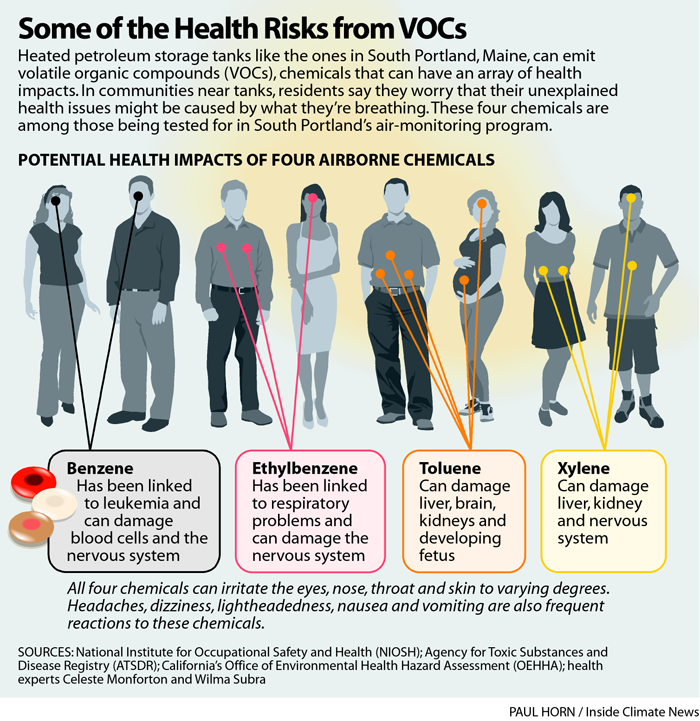
\includegraphics{fig/VOCs_Chemical_Health_Effects.png}

\href{https://insideclimatenews.org/news/18042021/toxic-neighbords-tank-fumes-epa-harmful-chemicals/}{Inside Climate News}

\hypertarget{effect-on-marine-life}{%
\subsection{Effect on Marine Life}\label{effect-on-marine-life}}

\textbf{Regulators missing pollution's effect on marine life, study finds}

Increasing chemical and plastic pollution are ``significant'' contributors to the decline of fish and other aquatic organisms, yet their impact is being missed by regulators.
The report, \href{https://ipen.org/transfer/embargo/aquatic_pollutants_in_oceans_and_fisheries_ipen-en.pdf}{Aquatic Pollutants in Oceans and Fisheries}, by the International Pollutants Elimination Network and the National Toxics Network, draws together scientific research on how pollution is adversely affecting the aquatic food chain. It catalogues the ``serious impacts'' of ``invisible killers'' such as persistent organic pollutants and excessive nutrients on the immunity, fertility, development and survivaL of aquatic animals.

Regulation of fisheries does not always take into account biologically or scientifically relevant data on all contributors to the health of fish populations, leading to a ``narrow view'' of declining numbers based on quota catch rates and efforts. ``Regulators have yet to grasp the impact of pollution,'' the report says.

\href{https://www.theguardian.com/environment/2021/apr/27/regulators-missing-pollutions-effect-on-marine-life-study-finds}{Guardian}

\hypertarget{pesticides}{%
\subsection{Pesticides}\label{pesticides}}

\emph{Jones}

When different pesticides mix together, as they often do on farms, they can amplify the effect of one another, according to a new \href{https://www.nature.com/articles/s41586-021-03787-7}{study} published in the journal Nature. In deadly combination, they can be even more damaging to bees. \href{https://www.fisheries.noaa.gov/feature-story/pesticide-mixtures-deadly-synergy-salmon}{Previous research} has found that these ``synergies'' can harm fish and other creatures, too.

What's most troubling is that regulators in the US and elsewhere don't take the dangers of these interactions fully into account --- even though they've long been aware of them. The Environmental Protection Agency, which oversees pesticides in the US, effectively ignored a recommendation to determine which chemicals farmers most commonly mix together, and what risk those combinations pose to bees. Europe is making more progress, but its regulations still fall short, experts say.

So how exactly do things like pesticides and parasites interact to harm bees?

Siviter and his co-authors answered that question through a meta-analysis, which is essentially a study of studies. First, they combed scientific literature about how multiple stressors affect bees, ultimately turning up 90 papers that had relevant data. They then pooled the results in a large analysis in their own paper that shows which combinations are most deadly.

The analysis revealed especially bad news about pesticides. When present together, multiple chemicals can amplify the effect of one another, the analysis found, making them more deadly than you'd expect if you just added up the sum of their individual effects. (Pesticides, which include insecticides, fungicides, and herbicides, work in a variety of different ways; many insecticides target insects' immune systems.)

All of this matters so much because study after study finds that insects are exposed to more than one chemical at a time. ``When we look for pesticides, whether it's in our water or on our pollinator plants, we're finding them in mixtures,'' Code said.

A \href{https://pubmed.ncbi.nlm.nih.gov/28968582/}{study from 2018}, for example, found as many as seven pesticides per sample of pollen collected by honeybees in Italy, while \href{https://www.sciencedirect.com/science/article/abs/pii/S0269749121001445\#}{other research} has found residue from more than 20 chemicals in US hives.

The root of the problem may be bureaucracy, not biology. Regulations in the US and Europe have been slow to consider the impacts of pesticide mixtures on pollinator health. To register a chemical, companies typically don't have to test how it might interact with other compounds found on a farm or in the environment.

When doctors prescribe medicines, they're carefully attuned to the ways that different drugs could interact. We would not accept a doctor who didn't understand the impacts of mixing those medicines. We shouldn't accept it for our pesticides either.

\href{https://www.vox.com/22612979/pesticide-mixtures-kill-bees-insects-pollinators}{Jones (2021) Pesticides can amplify each other. Bees have become the victims.}

\hypertarget{sewage}{%
\section{Sewage}\label{sewage}}

\hypertarget{overflows}{%
\subsection{Overflows}\label{overflows}}

Raw sewage had been pumped into English rivers via storm overflows more than 200,000 times in 2019. In November, Surfers Against Sewage (SAS) published \href{https://www.theguardian.com/environment/2020/nov/06/raw-sewage-dumped-into-english-and-welsh-beaches-2900-times-this-year}{data} showing that untreated wastewater was discharged on to English and Welsh beaches on 2,900 occasions in a year.

The Environment Agency published, for the first time, full \href{https://www.theguardian.com/environment/2021/mar/31/water-firms-discharged-raw-sewage-into-english-waters-400000-times-last-year}{data} on raw sewage discharges last year, showing a 37\% year-on-year increase: 3.1m hours of human effluent flows, pumped via storm drains into English waters in some 400,000 occasions.

The prevalence of raw sewage in British waters is not only about the horror of swimming amid human waste but about the health and environmental threats of microplastics (especially from laundry water), endocrine disruptors (chemicals that interfere with hormones found in plastics, detergents and cosmetics), phosphorus (which causes algae blooms), antibiotic-resistant bacteria and even Covid-19 -- all spread through wastewater.

Good days are increasingly rare. Previously, only freak storms would fill the system to the point that the toxic soup would spill out into waterways (to avoid the even grislier prospect of it spouting back up our drains).

Vast tanks, such as those under the promenades in Blackpool and Brighton, have been built to hold excess stormwater, so it can be fed back into sewers once the water levels in the sewers drop. But this ``grey infrastructure approach'' is not a long-term solution.

\textbf{Sustainable Drainage Systems (SuDS)}

A key example of green infrastructure solutions are \emph{sustainable drainage systems}, known as SuDS. These allow the environment to absorb, slow and divert water. They use wetlands, ponds and green ditches called swales, as well as green roofs, rainwater-harvesting systems and replacing nonabsorbent surfaces with porous asphalt or gravel.

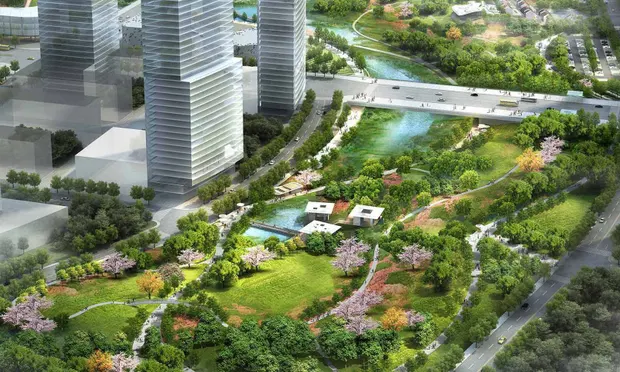
\includegraphics{fig/Wuhan-Storm_Corridor.png}

\emph{Figure: Xinyuexie Park, Wuhan, China, designed to improve a natural storm corridor.}

SuDS have been used to stunning effect in China, where flood-prone cities, such as Wuhan, have come to be known as ``sponge cities'', full of beautiful, biodiverse parkland that holds on to water. Other examples include Malmö in Sweden, which blazed a trail for ``blue-green cities'' at the turn of the century after introducing a series of trenches, ponds and wetlands to absorb up to 90\% of its stormwater. Davis says the Environment Agency is also looking at ``Copenhagen, as well as some of the American and Canadian examples -- Seattle and Vancouver -- where they're trying these different approaches''.

\textbf{Fuzzy Logic Network}

SuDS and concrete tanks are not the only weapons in the anti-sewage spill arsenal. Fatbergs and other blockages can trigger sewage pollution events, so having a better idea of what's going on underground is essential. Harrison says Yorkshire Water is working with Siemens on a \href{https://www.waterindustryjournal.co.uk/fuzzy-logic-clear-up-blockage-prediction-for-yorkshire-water}{pilot ``fuzzy logic'' network} around Ilkley, which uses real-time rainfall data, AI and sensors to better predict blockages. So far, the project has been able to predict nine out of 10 blockages -- three times more accurate than existing statistical modelling -- while reducing false alarms by half.

\textbf{Flushless Toilets}

A more radical solution to the sewage crisis is to do away with sewers altogether.

For people with gardens, waste would be sanitised and deodorised within the toilet unit, ``and the end-product would be made available directly to the user: this would likely involve heat-treatment as the best way to stabilise and dewater the waste as much as possible''. The sanitised waste could then be added to compost heaps.

Another concept is to use a municipal collection system where the product is combined with garden or food waste collections.

The nano-membrane toilet, developed by Cranfield University. Liquids undergo evaporation, killing many pathogens in the process, and can then be used for washing or irrigation, while solids are burned, producing enough energy to power the unit.
Fails to recover some of the useful resources in human waste.

\href{https://www.theguardian.com/environment/2021/apr/19/sewage-island-how-britain-spews-untreated-waste-rivers-sea}{Guardian -Sewage Island: How Britain spews sewage into sea}

\hypertarget{genetic-pollution}{%
\section{Genetic Pollution}\label{genetic-pollution}}

\textbf{Study on DNA spread by genetically modified mosquitoes prompts backlash}

For 10 years, the company Oxitec has been testing whether genetically modified (GM) mosquitoes can suppress populations of their natural brethren, which carry devastating viruses such as Zika and dengue. Its strategy: Deploy (nonbiting) male Aedes aegypti mosquitoes bearing a gene that should doom most of their offspring before adulthood.

Now, a team of independent researchers analyzing an early trial of Oxitec's technology is raising alarm---and drawing fire from the firm---with a report that some offspring of the GM mosquitoes survived and produced offspring that also made it to sexual maturity. As a result, local mosquitoes inherited pieces of the genomes of the GM mosquitoes, the team revealed last week in \href{https://www.nature.com/articles/s41598-019-49660-6}{Scientific Reports}.

There's no evidence that these hybrids endanger humans more than the wild mosquitoes or that they'll render Oxitec's strategy ineffective, both the paper's authors and the company agree. ``The important thing is something unanticipated happened,'' says population geneticist Jeffrey Powell of Yale University, who did the study with Brazilian researchers. ``When people develop transgenic lines or anything to release, almost all of their information comes from laboratory studies. \ldots{} Things don't always work out the way you expect.''

But the paper's suggestion that this genetic mixing could have made the mosquito population ``more robust''---more resistant to insecticides, for example, or more likely to transmit disease---has triggered anti-GM news reports, a backlash from some scientists, and strong pushback from Oxitec. The company, a subsidiary of U.S. biotech Intrexon, has a lot at stake; it recently submitted a new generation of its GM mosquitoes for U.S. regulatory review and hopes to conduct its first U.S. field test next year.

Even before Oxitec conducted pilot releases of its altered mosquitoes in Brazil, Malaysia, and the Cayman Islands, it knew the inserted gene wasn't inevitably lethal. Lab tests had shown that when the GM males mated with wild females, roughly 3\% of their offspring survived. ``We've been very clear about that,'' Rose says.

What wasn't clear was whether those rare offspring, often sickly in the lab, could themselves produce progeny, Powell says. To see whether the survivors fared well enough in the wild to spread their DNA, he contacted Oxitec's collaborators on the eve of a large field trial in the Brazilian city of Jacobina. From 2013 to 2015, Oxitec released roughly 450,000 GM male mosquitoes per week there---which the company reported reduced the overall mosquito population by about 90\%. Powell and his collaborators collected mosquitoes from several neighborhoods before, during, and in the 3 months after the trial. Within these populations, they estimate, between 5\% and 60\% of the insects had some DNA from the Oxitec strain in their genome---as much as 13\% of the genome in one case.

Oxitec's latest strain of GM mosquitoes is designed to spread the lethal gene more effectively. Instead of killing offspring regardless of sex, it eliminates only the females. Male offspring survive to pass on the lethal gene. In a Brazilian field trial, these second-generation mosquitoes caused local populations to dip by as much as 96\%, Oxitec announced in June.

\href{https://www.sciencemag.org/news/2019/09/study-dna-spread-genetically-modified-mosquitoes-prompts-backlash}{Servick in Science}

\hypertarget{light-pollution}{%
\section{Light Pollution}\label{light-pollution}}

\emph{Guardian}

\textbf{Transition to blue light radiation across Europe increases suppression of sleep hormone melatonin}

The orange-coloured emissions from older sodium lights are rapidly being replaced by white-coloured emissions produced by LEDs.
The increased blue light radiation associated with it is causing ``substantial biological impacts''.

Chief among the health consequences of blue light is its ability to suppress the production of melatonin, the hormone that regulates sleep patterns in humans and other organisms.

The increase in blue light radiation in Europe has also reduced the visibility of stars in the night sky, which the study says ``may have impacts on people's sense of nature''. Blue light can also alter the behavioural patterns of animals including bats and moths, as it can change their movements towards or away from light sources.

Local street lighting has dramatically reduced the abundance of nocturnal insect populations.

Light pollution can dramatically impact invertebrates, whether that be how they go about their daily lives, or even by reducing populations of species that live in habitats lit by LED lights. Given that invertebrates are already suffering dramatic declines, it is vital that we relieve them from all pressures to provide the best chance of recovery.

We should consider light from a wider biological perspective than that of just humans {[}and{]} we must focus on better quality lighting that is harmonious with our natural world. Better quality and lower levels of lighting would help save energy, and lower financial costs, while also making our environment safer for invertebrates.

National targets to reduce levels of light pollution are needed.
Measurements are patchy and uncoordinated.

\href{https://www.theguardian.com/environment/2022/sep/14/increase-in-led-lighting-risks-harming-human-and-animal-health}{Guardian (2022) Increase in LED lighting `risks harming human and animal health'}

\emph{Sanchez de Miguel Abstarct}

The nighttime environment of much of Earth is being changed rapidly by the introduction of artificial lighting. While data on spatial and temporal variation in the intensity of artificial lighting have been available at a regional and global scale, data on variation in its spectral composition have only been collected for a few locations, preventing variation in associated environmental and human health risks from being mapped. Here, we use imagery obtained using digital cameras by astronauts on the International Space Station to map variation in the spectral composition of lighting across Europe for 2012--2013 and 2014--2020. These show a regionally widespread spectral shift, from that associated principally with high-pressure sodium lighting to that associated with broad white light-emitting diodes and with greater blue emissions. Reexpressing the color maps in terms of spectral indicators of environmental pressures, we find that this trend is widely increasing the risk of harmful effects to ecosystems.

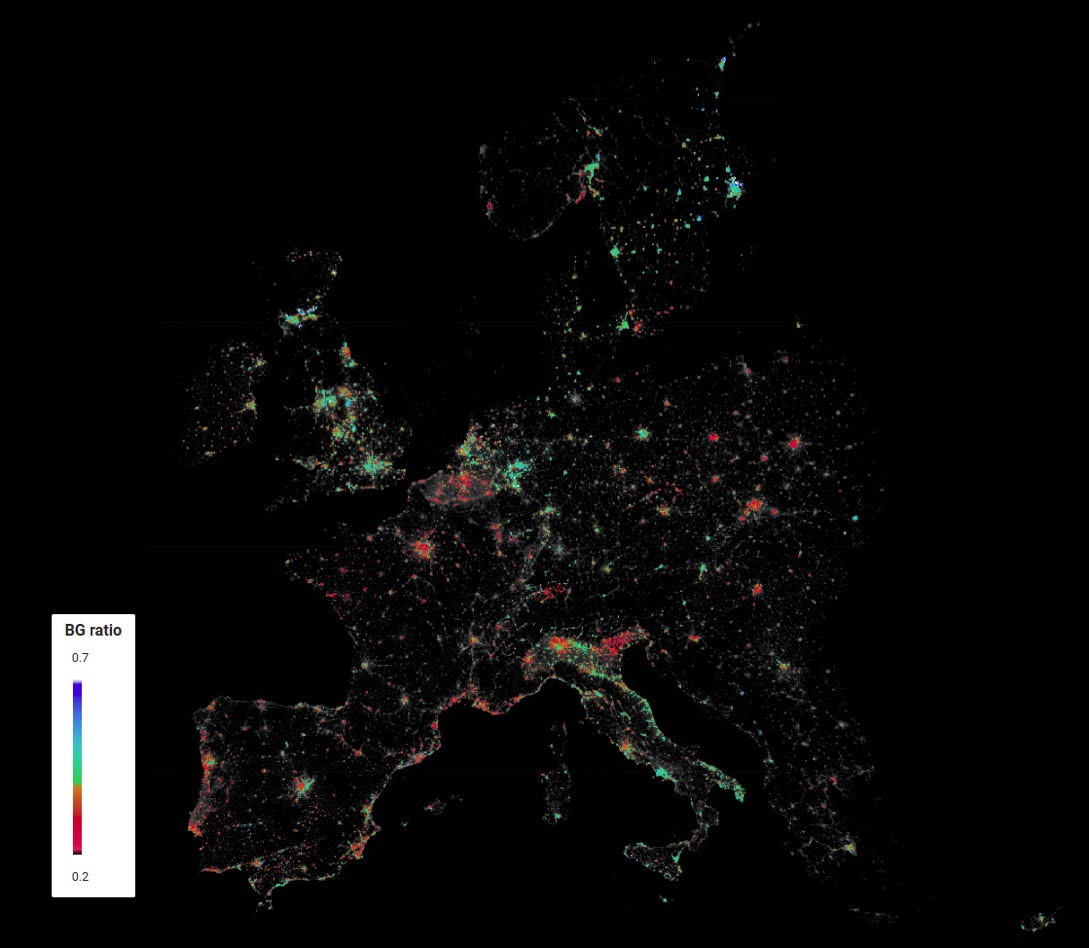
\includegraphics{fig/Light_Pollution_Europe.png}

\href{https://www.science.org/doi/10.1126/sciadv.abl6891}{Sanchez de Miguel (2022) Environmental risks from artificial nighttime lighting widespread and increasing across Europe}
\href{pdf/Sanchez-de_Miguel_2022_Environmetal_Risks_from_Artificalial_Nighttime_Lightning.pdf}{(pdf)}
\href{pdf/Sanchez-de_Miguel_2022_Environmetal_Risks_from_Artificalial_Nighttime_Lightning_SI.pdf}{(pdf SI)}

\hypertarget{species}{%
\chapter{Species}\label{species}}

\hypertarget{birds}{%
\section{Birds}\label{birds}}

\emph{Guardian}

Researchers pored over data collected since the mid-60s in Britain and the Netherlands on 60 different species, including the house sparrow, the crested tit, the reed bunting, the bullfinch and the willow warbler. They zero in on how these birds have changed over time with regard to their egg-laying schedules, number of offspring and morphology.

The scientists investigated what proportion of changes over time were linked to warming, and whether warming affected some species or traits more than others, as well as whether other factors unrelated to temperature reinforced these effects.

\href{https://www.theguardian.com/environment/2022/mar/10/climate-change-fundamentally-affecting-european-birds-study-shows}{Guardian (2022) Climate change fundamentally affecting European birds}

\emph{McLean Abstract}

Many wild populations are experiencing temporal changes in life-
history and other phenotypic traits, and these changes are fre-
quently assumed to be driven by climate change rather than
nonclimatic drivers. However, this assumption relies on three con-
ditions: that local climate is changing, traits are sensitive to climate
variability, and other drivers are not also changing over time.
Although many studies acknowledge one or more of these condi-
tions, all three are rarely checked simultaneously. Consequently,
the relative contribution of climate change to trait change, and the
variation in this contribution across traits and species, remain
unclear. We used long-term datasets on 60 bird species in Europe
to test the three conditions in laying date, offspring number, and
body condition and used a method that quantifies the contribu-
tion of warming temperatures to changes in traits relative to other
effects. Across species, approximately half of the magnitude of
changes in traits could be attributed to rising mean temperature,
suggesting that increasing temperatures are likely the single most
important contributor to temporal trends and emphasizes the
impact that global warming is having on natural populations.
There were also substantial nontemperature-related temporal
trends (presumably due to other changes such as urbanization),
which generally caused trait change in the same direction as
warming. Attributing temporal trends solely to warming thus
overestimates the impact of warming. Furthermore, contributions
from nontemperature drivers explained most of the interspecific
variation in trait changes, raising concerns about comparative
studies that attribute differences in temporal trends to species dif-
ferences in climate-change sensitivity.

\href{https://www.pnas.org/doi/epdf/10.1073/pnas.2105416119}{McLean (2022) Warming temperatures drive at least half of themagnitude of long-term trait changes inEuropean birds}
\href{pdf/McLean_2022_Warming_Bird_Traits.pdf}{(pdf)}

\hypertarget{polar-bear}{%
\section{Polar Bear}\label{polar-bear}}

\emph{Today}

Polar bears are among the few large carnivores that are still found in roughly their original habitat and range--and in some places, in roughly their natural numbers.

Although most of the world's 19 populations have returned to healthy numbers, there are differences between them. Some are stable, some seem to be increasing, and some are decreasing due to various pressures.

Status of the polar bear populations
Updated 2019 with data from the IUCN Polar Bear Specialists Group

\begin{verbatim}
4 populations are in decline
2 populations are increasing
5 populations are stable
8 populations are data-deficient (information missing or outdated)
\end{verbatim}

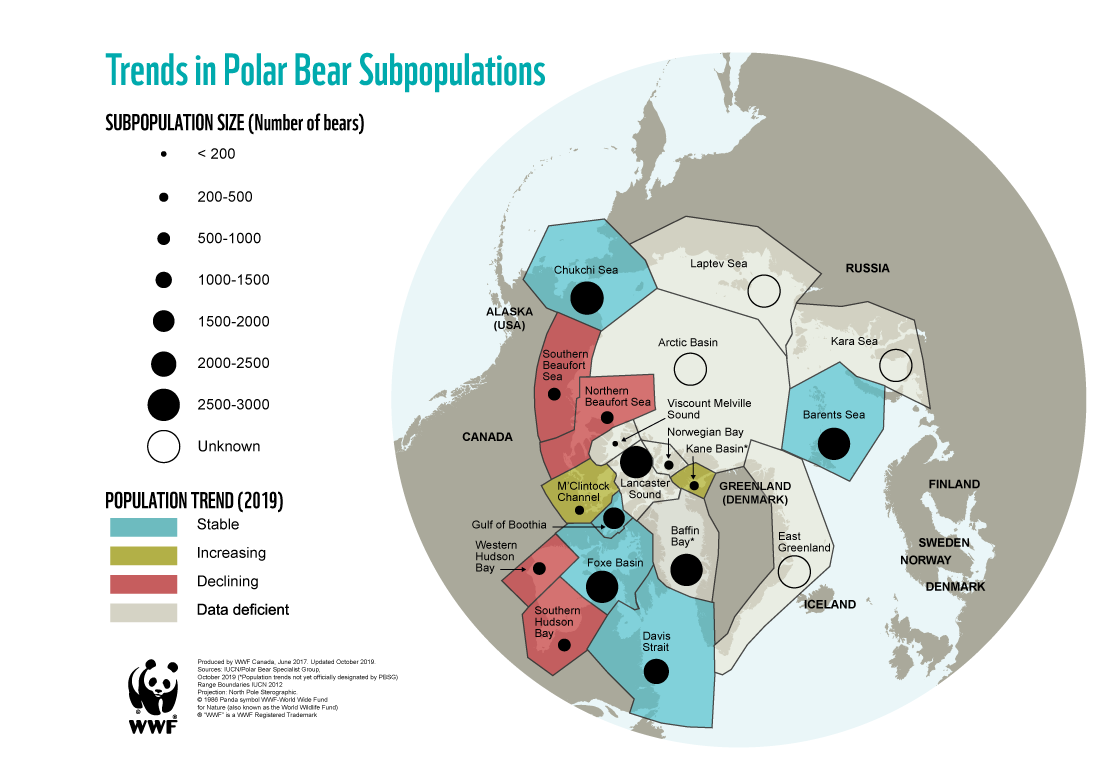
\includegraphics{fig/polar_bear_populations.png}

\emph{In the future}

By 2040, scientists predict that only a fringe of ice will remain in Northeast Canada and Northern Greenland when all other large areas of summer ice are gone. This ``Last Ice Area'' is likely to become important for polar bears and other life that depends on ice.

A projection of sea ice in the archipelago, supported by WWF, shows that much of the region is facing significant ice loss in the coming decades - with potentially serious consequences for polar bears.

Global polar bear numbers are projected to decline by 30\% by 2050.

\href{https://arcticwwf.org/species/polar-bear/population/}{WWF}

\emph{Polar Bear Threatened at Svalbard}

Dag Vongraven er ekspert på isbjørn. I elleve år har han ledet en internasjonal gruppe med spesialister på den hvite kjempen, International Union for Conservation of Nature (IUCN).

Før han nå gir ledervervet videre, tegner han et dystert bilde av isbjørnens fremtid.

-- Jeg er redd for at den kommer til å være helt borte fra Svalbard om 50 år.

Vongraven mener vi nå er i starten av en periode som vil føre til isbjørnens utryddelse på Svalbard, om oppvarmingen fortsetter i samme tempo som de siste tiårene.

Årsaken til hans dystre spådom er polhavet og havisen som smelter raskere enn før.

Oppvarmingen skjer dobbelt så raskt som for 25 år siden.

Om femti år frykter Vongraven at flerårsisen vil være helt borte, og isbjørnen med den.

Lite havis = lite mat

Havisen er viktig for isbjørnen. Slik transporterer den seg mellom områder der det er mat og mellom steder der den kan finne hi, forteller isbjørneksperten.

-- Isbjørn klarer ikke å fange ringsel på landet eller i vann. Den er tilpasset til å fange ringsel på isen, sier Vongraven.

Det finnes i dag rundt 26.000 isbjørner i verden, fordelt på 19 ulike delbestander. Barentshavbestanden er mellom 1900 og 3600 isbjørn, ifølge tall fra Norsk Polarinstitutt.

På Svalbard er det cirka 300 «fastboende» isbjørner.

-- Det går linjer tilbake, fra Svalbardtraktaten i 1920, via Svalbardmiljøloven og fram til i dag der det står at man skal bevare dyrelivet på Svalbard. Isbjørnen er selve kroneksempelet på hvor viktig dette er.

Innen 50 år har gått så har vi to tredeler færre isbjørn. Den nye rødlistevurderingen fra gruppa jeg har ledet viser det samme. Det er store endringer, og det er forferdelig trist å jobbe med dette og se utviklingen vi står overfor.

\href{https://www.nrk.no/tromsogfinnmark/mener-isbjorn-kan-vaere-utryddet-pa-svalbard-om-50-ar-1.15559199}{nrk}

\hypertarget{pandemics}{%
\chapter{Pandemics}\label{pandemics}}

\hypertarget{loss-of-habitat-as-a-driver}{%
\section{Loss of habitat as a driver}\label{loss-of-habitat-as-a-driver}}

Som text on the linksbetween loss of biodiversity and pandemics

\begin{quote}
Almost all pandemics start with a single infection event. For zoonoses from wildlife, this is a person, or group of people that made contact with an animal infected by a pathogen that infects them, replicates in their cells and then is transmitted to others. Surveillance data suggest that spillover events happen frequently around the world, but most infections are unable to cause further transmission among people. Sometimes, pathogens spill over and are able to transmit to a handful of people, undergoing a few cycles of transmission before the outbreak dies out. Where pathogens spread into dense human communities (e.g.~COVID-19 within the live animal market and city of Wuhan 10 ), and when they are able to easily transmit from person-to-person, they can become pandemics. Preventing pandemics will require efforts to reduce the risk each of these stages occurring, through measures that diminish the underlying drivers of spillover, their spread among people and their ability to move globally through rapidly urbanizing landscapes, megacities and travel and trade networks.
\end{quote}

\begin{quote}
Pandemics represent an existential threat to the health and welfare of people across the planet, and their emergence, impact and control are deeply embedded in biodiversity and the major causes of biodiversity loss. New diseases emerge largely in tropical or subtropical countries with high wildlife biodiversity. The first people to be infected are often from communities in remote or rural regions, in developing countries with lower capacity to rapidly diagnose and treat novel diseases, and control and contain pandemic spread. Land use change and the wildlife trade (especially unsustainable, illegal or poorly regulated wildlife trade) are key drivers of pandemic emergence, including the recent emergence of COVID-19. Pandemics, such as COVID-19, underscore both the indivisible interconnectedness of the world community and the rising threat posed by global inequality to the health, wellbeing and security of all people: Exponential growth in consumption of products from land use change and globalized trade, often driven by developed countries, have led to the repeated emergence of diseases from developing countries with high biodiversity, and thus conditions that increase potential for zoonotic emergence.
\end{quote}

\hypertarget{bats-habitat-loss-drives-diseases}{%
\subsection{Bats habitat loss drives diseases}\label{bats-habitat-loss-drives-diseases}}

Many of the recently emerging highly virulent zoonotic diseases have a
likely bat origin, for example Hendra, Nipah, Ebola and diseases caused
by coronaviruses.
Presumably because of their long history of coevolution, most of these
viruses remain subclinical in bats,
but have the potential to cause severe illnesses
in domestic and wildlife animals and also humans.

Increasing numbers of breakouts of zoonotic viral diseases among
humans and livestock have mainly been accounted to human encroachment
into natural habitat, as well as agricultural intensification,
deforestation and bushmeat consumption.
Persecution of bats, including the destruction of their roosts and culling of
whole colonies, has led not only to declines of protected bat species,
but also to an increase in virus prevalence in some of these populations.

\href{https://www.researchgate.net/publication/286449572\%20_Zoonotic_Viruses_and_Conservation_of_Bats}{Zoonotic Diseases and Conservation of Bats}
\href{/pdf/Schneeberger_Voigt_2016_Bats_Zoonotic.pdf}{(pdf)}

\href{https://www.bbc.com/future/article/20210106-nipah-virus-how-bats-could-cause-the-\%20next-pandemic}{Nipah (BBC)}

\hypertarget{apolitical-public-health}{%
\section{Apolitical Public Health}\label{apolitical-public-health}}

\emph{Memo}

Global health is a discipline that holds within itself a deep contradiction---global health was birthed in supremacy, but its mission is to reduce or eliminate inequities globally.

Most epidemiological analyses and modeling studies to be devoid of any analyses of power. ``For the most part, epidemiology as a method of science is considered apolitical; it actually serves as an ideological apparatus of imperialism by shielding structural causes of health inequities in the Global South,''

Epidemiological analyses of disease dynamics that fail to consider sociohistorical forces. In doing so, these studies end up diverting the public's gaze from legacies of colonialism, white supremacy, structural adjustment, institutional racism, and purposeful under-development which leaves health systems so weak and ineffective.

Move away from the notion of a universal truth.
Reject the notion that social inquiry can produce objective, value-neutral, and univocal understanding. Instead, we must embrace the critical and the polyvocal.

\href{https://naturemicrobiologycommunity.nature.com/posts/a-mind-bending-take-on-the-coloniality-of-global-public-health}{Epidemic Illusions}

\hypertarget{pandemic-risk-management}{%
\section{Pandemic Risk Management}\label{pandemic-risk-management}}

\emph{Memo}

We are dealing with an extreme fat-tailed process owing to an increased connectivity,
which increases the spreading in a nonlinear way.
Fat tailed processeshave special attributes, making conventional risk-management
approaches inadequate.

The general (non-naive) precautionary principle delineates conditions where actions
must be taken to reduce risk
of ruin, and traditional cost-benefit analyses must not be used.
These are ruin problems where, over time, exposure to tail
events leads to a certain eventual extinction. While there
is a very high probability for humanity surviving a single
such event, over time, there is eventually zero probability of
surviving repeated exposures to such events. While repeated
risks can be taken by individuals with a limited life expectancy,
ruin exposures must never be taken at the systemic and
collective level. In technical terms, the precautionary principle
applies when traditional statistical averages are invalid because
risks are not ergodic.

Estimates of the virus's reproductive
ratio \$R\_\{0\} - the number of cases one case generates on average
over the course of its infectious period in an otherwise
uninfected population - are biased downwards. This property
comes from fat-tailedness {[}4{]} due to individual `superspreader'
events. Simply, R 0 is estimated from an average which takes
longer to converge as it is itself a fat-tailed variable

Standard individual-scale policy approaches
such as isolation, contact tracing and monitoring are rapidly
(computationally) overwhelmed in the face of mass infection,
and thus also cannot be relied upon to stop a pandemic. Multi-
scale population approaches including drastically pruning con-
tact networks using collective boundaries and social behavior
change, and community self-monitoring, are essential.
Together, these observations lead to the necessity of a
precautionary approach to current and potential pandemic
outbreaks that must include constraining mobility patterns in
the early stages of an outbreak, especially when little is known
about the true parameters of the pathogen.
It will cost something to reduce mobility in the short term,
but to fail do so will eventually cost everything---if not from
this event, then one in the future. Outbreaks are inevitable, but
an appropriately precautionary response can mitigate systemic
risk to the globe at large. But policy- and decision-makers must
act swiftly and avoid the fallacy that to have an appropriate
respect for uncertainty in the face of possible irreversible
catastrophe amounts to ``paranoia,'' or the converse a belief
that nothing can be done.

\href{https://necsi.edu/systemic-risk-of-pandemic-via-novel-pathogens-coronavirus-a-note}{Norman/Bar-Yam/Taleb Note}
\href{/pdf/Joseph_Norman_2020_Systemic_Risk_of_Pandemic_via_Novel_Pathogenes.pdf}{(pdf)}

\hypertarget{land-use}{%
\chapter{Land Use}\label{land-use}}

\hypertarget{agriculuture}{%
\section{Agriculuture}\label{agriculuture}}

Our industrial food boom spawned similar failures of systemic context. Our inventive, so-called green revolution of food solutions produced a lot of food and made profits for large corporations, but depleted soil nutrients, spread toxins, severed mycelial networks, and disrupted nutrient cycles, creating eutrophic lakes and dead zones in our oceans.

\href{https://mahb.stanford.edu/blog/thresholds-cascades-and-wicked-problems/}{Wicked Complexity}

\hypertarget{forests}{%
\section{Forests}\label{forests}}

\hypertarget{tropical-rainforest}{%
\subsection{Tropical Rainforest}\label{tropical-rainforest}}

Analysed and compiled Global Forest Watch data from all of the 73 countries
that are home to the world's tropical rainforests,
the planet's oldest and most diverse terrestrial ecosystem.

Of the approximately 14.5 million square kilometres of tropical rainforest that once covered Earth's surface, only 36 \% remains intact. Just over a third, 34 \%, is completely gone and the last 30 \% is in various forms of degradation.

Of the current rainforest cover, almost half (45 \%) is in a degraded state.

An area half the size of Europe is still completely intact.

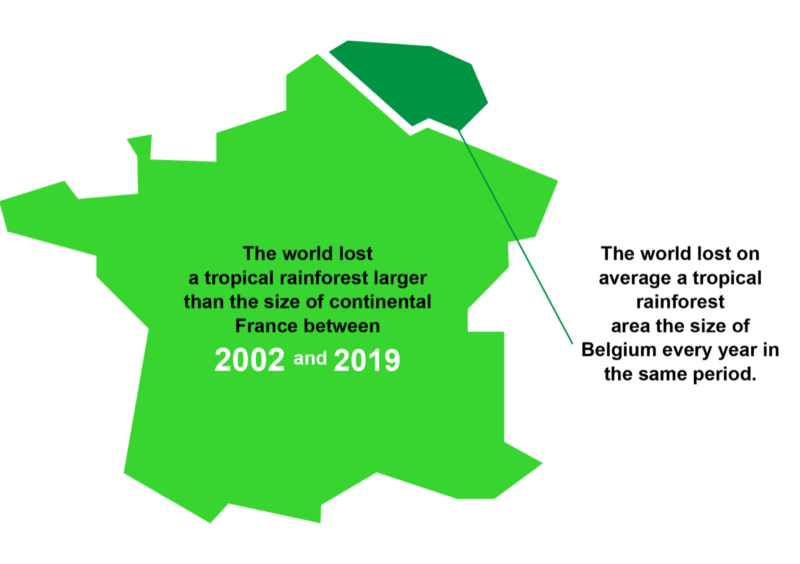
\includegraphics{fig/rainforest_loss_as_france_belgium.png}

The remaining tropical rainforests are either severely damaged or increasingly fragmented.
Humans are chopping these once vast and impenetrable forests into smaller and smaller pieces,
undermining their ability to store carbon, cool the planet, produce rain and provide habitats.

\href{https://www.regnskog.no/en/news/only-half-of-the-worlds-rainforests-remains-intact}{State of Tropical Rainforest Report 2020}

\hypertarget{deforestation-footprint}{%
\section{Deforestation Footprint}\label{deforestation-footprint}}

\emph{Carbonbrief}

Agriculture and forestry are responsible for 80\% of global deforestation.
This is mainly driven by demand for goods --
including coffee, chocolate, cattle, soy, palm oil and timber --
that are often then traded and consumed in countries around the world.

The UK, Germany, France, Italy and Japan ``imported'' more than
90\% of their national deforestation footprints from abroad between 2001 and 2015,
the study finds, of which between 46\% and 57\% was from tropical forests.

Residents in G7 countries drove an average loss of 3.9 trees or 58m2 of forest per capita through their consumption patterns in 2015, the results show, with the per-capita tree loss of the US in 2015 clocking in at twice that of Japan, Germany, France or the UK.

Tree loss in Singapore was almost entirely imported from south-east Asia, the study notes. Meanwhile, Brazilian deforestation was predominantly categorised as domestic -- although much of it was the result of producing goods that would be exported.

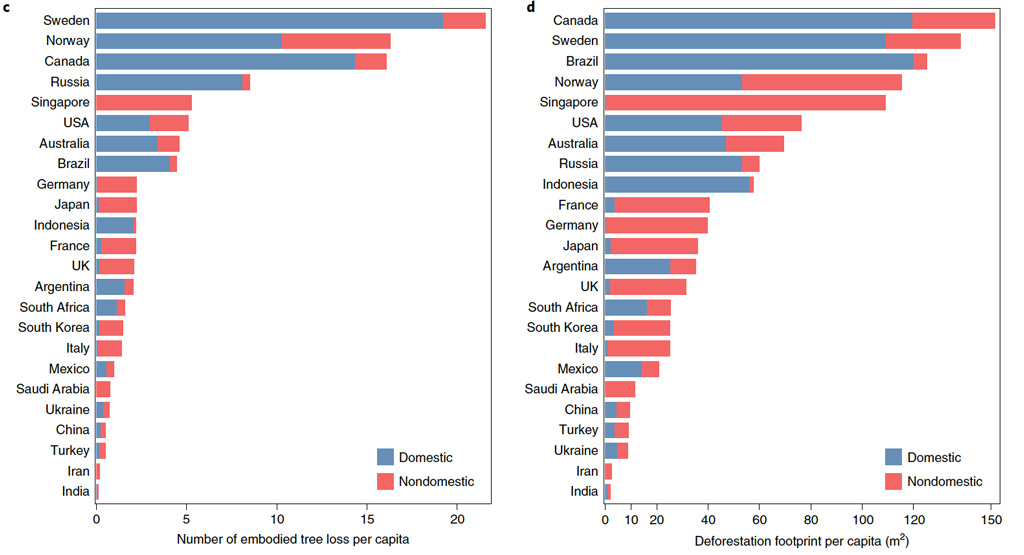
\includegraphics{fig/deforestaion_footprint.jpg}

Obtaining net forest gains domestically,
but expanding non-domestic deforestation footprints --
especially in the tropics -- might do more harm than good for climate change mitigation.

Deforestation is now one of the largest sources of greenhouse-gas emissions on the planet.

It's easy to look at the farmers, foresters and countries where deforestation is occurring and wish they would stop. But they are responding to signals from the global market. We are buying their soy as feed for our hamburgers and salmon and their palm oil as input to our lipstick.

\href{https://www.carbonbrief.org/scientists-calculate-trade-related-deforestation-footprint-of-rich-countries}{Carbonbrief (2021) On Hoang}

\emph{Hoang}

Deforestation, a significant threat to biodiversity, is accelerated by global demand for commodities. Although prior literature has linked deforestation to global supply chains, here we provide a fine-scale representation of spatial patterns of deforestation associated with international trade. Using remote sensing data and a multi-region input--output model, we quantify and map the spatiotemporal changes in global deforestation footprints over 15 years (2001--2015) at a 30-m resolution. We find that, while many developed countries, China and India have obtained net forest gains domestically, they have also increased the deforestation embodied in their imports, of which tropical forests are the most threatened biome. Consumption patterns of G7 countries drive an average loss of 3.9 trees per person per year. Some of the hotspots of deforestation embodied in international trade are also biodiversity hotspots, such as in Southeast Asia, Madagascar, Liberia, Central America and the Amazonian rainforest. Our results emphasize the need to reform zero-deforestation policies through strong transnational efforts and by improving supply chain transparency, public--private engagement and financial support for the tropics.

\href{https://www.nature.com/articles/s41559-021-01417-z}{Hoang (2021) Mapping Deforestation Footprint(Nature, paywall)}

\hypertarget{wetland}{%
\section{Wetland}\label{wetland}}

\emph{Global Wetland Outlook}

\href{https://www.global-wetland-outlook.ramsar.org/outlook}{Global Wetland Outlook 2021 Update}

-- Våtmarker lagrer over 30 prosent av alt landbasert karbon og er viktige for helse- mat- og vannsikkerhet.

Den internasjonale avtalen om våtmarker -- Ramsarkonvensjonen -- har lansert en ny spesialrapport om situasjonen for verdens gjenværende våtmarker, Global Wetland Outlook: Special Edition 2021.

Rapporten viser at vi fortsetter å ødelegge eller forringe våtmarkene i et alarmerende tempo. Globalt har 35 prosent av våtmarkene gått tapt siden 1970. Våtmarker er vårt mest truede økosystem, og de forsvinner tre ganger raskere enn skogene.

Våtmarker er vårt mest effektive landbaserte økosystem for å fange karbon. Torvmarker, som blant annet inkluderer det meste av norske myrer, dekker kun 3 prosent av jordens landoverflate, men lagrer ifølge rapporten likevel 30 prosent av alt landbasert karbon.

Hovedfunn fra rapporten:

\begin{itemize}
\tightlist
\item
  En fjerdedel av verdens våtmarksavhengige arter er i ferd med å bli utryddet.
\item
  Effektene av klimaendringer på våtmark kommer mye raskere enn forventet. Dette slår særlig ut i arktiske strøk og i fjellet, men også langs kysten.
\item
  Arealbruksendringer er den viktigste årsaken til at våtmarker har forsvunnet på land. Globalt har landbruk ødelagt eller forringet mer enn halvparten av verdens våtmarker.
\item
  Dårlig forvaltning av våtmarker har økt graden av vannmangel og vannbårne sykdommer, og det er anslått at dette bidrar til millioner av dødsfall hvert år.
\item
  Våtmark er mange steder avgjørende for tilpasning til et klima med våtere og villere vær, blant annet mangroveskog og torvmarker.
\item
  Intakte og velfungerende våtmarker er avgjørende for å nå de globale klimamålene, FNs bærekraftsmål og målene i det globale rammeverket for biologisk mangfold som skal vedtas i 2022.
\end{itemize}

\href{https://www.miljodirektoratet.no/aktuelt/nyheter/2021/desember-2021/vatmark-forsvinner-tre-ganger-raskere-enn-skogene/}{Miljødirektoratet (Norway)}

\hypertarget{soil}{%
\section{Soil}\label{soil}}

\textbf{SoilDepth}

No-till farming was developed and promoted in the mid-20th century as an erosion control measure. Under conventional tillage, soil is broken up and mixed mechanically. In no-till farming, soil disturbance is minimized and crop residues are left on the soil surface. Reducing or eliminating tillage improves water infiltration rates and protects against wind and water erosion. Reducing tillage also improves soil structure, allowing ``aggregates'' (intact clumps of soil) to form when they otherwise would have been broken into smaller pieces. Aggregates are often carbon rich, and are thought to have a role in protecting organic matter from decay.Although this suggests that eliminating or reducing tillage might be a way to increase the overall amount of carbon stored in soil, the relationship between tillage and soil carbon storage remains a heavily debated topic. No fewer than 11 synthesis papers published in the past five years have addressed the relationship between tillage and soil carbon storage.

These papers each analyzed data from hundreds of individual studies. While the synthesis papers analyzed many of the same studies, they reached a range of conclusions. Some have concluded that tillage has no statistically detectable effect on overall soil carbon storage, while others have identified positive effects or indicated that tillage effects depend on other factors such as climate and soil type

Sampling depth is likely a key source of the disagreement. It has two main effects, which we call the ``carbon redistribution effect'' and ``density change effect''. We'll describe each in turn.

\href{https://carbonplan.org/research/soil-depth-sampling}{carbinPlan}

\hypertarget{lakes}{%
\section{Lakes}\label{lakes}}

\hypertarget{mountains}{%
\section{Mountains}\label{mountains}}

\hypertarget{urban}{%
\section{Urban}\label{urban}}

\hypertarget{monoculture}{%
\chapter{Monoculture}\label{monoculture}}

\hypertarget{bananas}{%
\section{Bananas}\label{bananas}}

\hypertarget{panama-disease}{%
\subsection{Panama Disease}\label{panama-disease}}

In a long-feared development, an extremely damaging banana disease has apparently reached Latin America. Late last week, the Colombian Agricultural Institute (ICA) in Bogotá confirmed that four plantations in northern Colombia have been quarantined because of suspected infection with Fusarium wilt tropical race 4 (TR4), a fungus that kills plants by clogging their vascular system. Already widespread in Asia, the disease can wipe out entire plantations.

The finding has yet to be confirmed, but countries in the region are on high alert. Neighboring Ecuador is the largest banana exporter in the world; Colombia, Costa Rica, and Guatemala are big producers as well. A major outbreak of TR4 could ruin many farmers and drive up banana prices globally. ``It poses a big threat,'' says Rob Reeder, a plant pathologist at CABI, a nonprofit research and outreach center for plant diseases in the developing world, based in Egham, U.K. ``This should really start raising alarm bells.'' ``We should take this extremely seriously,'' adds Gert Kema, a plant pathologist at Wageningen University in the Netherlands.

TR4 is a variant of Panama disease, which wiped out banana plantations across Latin America in the mid-20th century. The industry recovered after it replaced the most widely cultivated banana variety at the time, Gros Michel---also known as the Big Mike---with a new one, the Cavendish, that is resistant to Panama disease and now dominates the export industry.

TR4, which easily overcomes the defenses of the Cavendish and many other banana varieties, emerged in Indonesia in the 1960s and has spread to many other countries since then. It surfaced in Jordan in 2013, in Mozambique 2 years later, and also in India, the world's largest banana producer. Scientists dreaded its jump to the Americas, suspecting it was only a matter of time.

\emph{Fusarium} is spread largely by contaminated soil and infected plant materials. It's possible that the strain arrived with farm machinery from abroad, or was carried by traveling farm workers or tourists. Banana leaves, used for wrapping food in many countries, are another potential infection route. (Bananas themselves do not spread the disease.)

New ways to battle the scourge are on the horizon. Adding certain types of biomass to the soil and covering it in plastic can kill the spores, as the material decomposes and releases gas toxic to bacteria and fungi. In trials conducted by Kema and his colleagues in the Philippines, the technique significantly reduced the number of spores, suggesting it might help contain the disease.

The longer-term solution is the same one that saved plantations decades ago: replacing the vulnerable plants with a resistant variety. The Honduras Foundation for Agricultural Research in La Lima has spent decades breeding TR4-resistant bananas, but so far the results have not lived up to the Cavendish in properties such as taste and resistance to blemishes. A genetically modified Cavendish produced in Dale's lab has shown resistance to the fungus in early field trials. Dale says that banana is now in larger trials; he hopes it can be commercialized in 2023. But whether consumers will buy transgenic bananas remains a question.

What's already clear from TR4's apparent arrival in Latin America, Kema says, is that banana cultivation cannot continue without major changes. ``This is a turning point for the industry,'' he says.

\href{https://www.sciencemag.org/news/2019/07/devastating-banana-disease-may-have-reached-latin-america-could-drive-global-prices}{Science}

\hypertarget{sea-use}{%
\chapter{Sea Use}\label{sea-use}}

Seaspiracy shows why we must treat fish not as seafood, but as wildlife.
(\citet{GeorgeMonbiot})

\hypertarget{actions}{%
\chapter{Actions}\label{actions}}

\begin{quote}
Desertification and climate change is happening so fast,
we need action on the ground.
Enough seminars, talks, talks, talks.
\end{quote}

\hypertarget{analysis}{%
\section{Analysis}\label{analysis}}

I remember thinking, in the 1970s, that once people became aware of the ecological crisis --- disappearing species, polluted rivers, poisoned air --- that the necessary changes would be simple to achieve. Humanity only had to curb industrial waste and destruction, preserve wilderness for other species, put limits on our consumption, stabilize human population, and just be smart about how to live on Earth without destroying it.

Of course, I was naive to think any of that would be easy. Since that time, human population has doubled, consumption of material resources has quadrupled, biodiversity collapse has accelerated, and after 34 international climate meetings, we are emitting more carbon than ever before. Meanwhile, we have not exactly ended war, vanquished racism, nor achieved gender or economic parity. Even worse, giant corporate interests actively work to halt and reverse any ecological regulation on industrial activity.

Our emotional responses to crisis evolved over millennia, primarily to meet immediate needs, perhaps to benefit our tribe or community, not necessarily to solve complex, multi-dimensional, long-term dilemmas. Our ideas about ``solutions'' tend to be linear, short-term, and linked to a perception of simple cause and effect. Our educational institutions encourage this linear thinking about problems and solutions. Meanwhile, our social and ecological challenges are systemic, multidimensional, and complex.

Living ecosystems are dynamic, always changing, and possess qualities such as thresholds, cascades, feedback loops, tipping points, lags, and generally unintended consequences to input. Maybe we need to learn more about how change actually occurs in nature, not just in our imaginations or in our engineering dissertations.

\href{https://mahb.stanford.edu/blog/thresholds-cascades-and-wicked-problems/}{Wicked Complexity}

\hypertarget{actionism}{%
\section{Actionism}\label{actionism}}

\begin{quote}
Any activist group needs a sound theory of change and a clear strategy for gaining influence.
\end{quote}

\href{https://jacobinmag.com/2020/12/climate-change-protest-strategy-electoral-politics-sunrise-extinction-rebellion}{Organizing Actions (Edward Carver on Sunrise and XR)}

\hypertarget{bankrolling}{%
\section{Bankrolling}\label{bankrolling}}

\emph{Bankrolling} is about making finance institutions responsible for the environmental
impacts of what they finance.

\hypertarget{bankrolling-plastics}{%
\subsection{Bankrolling Plastics}\label{bankrolling-plastics}}

Banks are failing to address the global plastic-pollution crisis,
having provided \$1.7 trillion in financing to packaging companies, retailers and
related businesses.

The banks haven't put in place due-diligence processes for packaging companies or
made funding contingent on policies that reduces plastic and favors recycling
over virgin plastics.

Banks are currently not taking any responsibility to understand, measure or reduce
the impacts of their loans within the plastics value chain.
By indiscriminately funding actors in the plastics supply chain, banks have failed
to acknowledge their role in enabling global plastic pollution.

Banks need to mitigate their role in enabling plastic pollution in a number of ways
-- for example, by aligning their lending portfolios with public policy
on plastic reduction, reusability and recycling,
and ceasing the financing of new plants that use virgin feedstock
to produce single-use plastic packaging.

\href{https://www.bloomberg.com/news/articles/2021-01-07/banks-directed-1-7-trillion-to-firms-causing-plastic-pollution}{Bloomberg News}

\href{https://portfolio.earth/}{Portfolio Earth}

\hypertarget{bankrolling-extinction}{%
\section{Bankrolling Extinction}\label{bankrolling-extinction}}

\emph{Memo}

It is clear banks
do not consider
themselves
responsible
or liable for
biodiversity
impacts caused
by their lending
activities

In 2019 the world's largest banks invested more than USD 2.6 trillion (equivalent to Canada's GDP) in sectors governments and scientists agree are the primary drivers of biodiversity destruction.

The financial sector is bankrolling the mass extinction crisis, while undermining human rights and indigenous sovereignty.

We are currently in the midst of a mass
extinction event. Termed the `Anthropocene
Extinction', this is the first of its kind to be
caused by humans. Humans have impacted
nearly every corner of the planet and are
approaching planetary boundaries which
could take millions of years to recover
from. 1 Scientists are warning of `biological
annihilation'. 2 While governments and
companies have been the focus of attention
on this issue, actors in the finance sector
have largely evaded scrutiny until recently.

The report calls for:

\begin{itemize}
\tightlist
\item
  Banks to disclose and radically reduce their
  impact on nature and stop finance for new
  fossil fuels, deforestation, overfishing and
  ecosystem destruction.
\end{itemize}

-Governments to stop protecting banks' role
in biodiversity destruction and rewrite the
rules of finance to hold banks liable for the
damage caused by their lending.

\begin{itemize}
\tightlist
\item
  People everywhere to have a say in how
  their money is invested, and a right to stop
  banks from causing serious harm to people
  and planet.
\end{itemize}

We cannot rely on banks to find the answer. We need
a radical overhaul of how our financial system creates
liability, accountability, and responsibility to protect
and restore nature.

To prevent extinction, banks have to stop
funding it.

\href{https://portfolio.earth/campaigns/bankrolling-extinction/}{bankrolling Extinction}

\hypertarget{heros}{%
\section{Heros}\label{heros}}

\href{https://edition.cnn.com/2020/12/31/world/new-years-resolution-2021-heal-nature-c2e-spc-intl/index.html}{Environmental Heros 2020 (CNN)}

\hypertarget{rewilding}{%
\section{Rewilding}\label{rewilding}}

\href{https://edition.cnn.com/2020/10/01/world/knepp-farm-rewilding-scn-cte-spc/index.html}{Kent Farm rewilds}

\hypertarget{conservation}{%
\section{Conservation}\label{conservation}}

\emph{Guardian}

About 17\% of land and inland water ecosystems and 8\% of marine areas are within formal protected areas, with the total coverage increasing by 42\% since the beginning of the last decade, according to the \href{https://livereport.protectedplanet.net/}{Protected Planet report} by the UN Environment Programme (Unep) and International Union for Conservation of Nature (IUCN).

The Protected Planet report is the final report card on \href{http://url3193.iucn-crm.org/ls/click}{Aichi Target 11} -- the global 10-year target on protected and conserved areas. The UN calculated that 16.64\% of land and inland waters has been protected to date but concluded that governments had met the 17\% target because of a lag in reporting on data. The 17\% ambition was just one of seven parts of Aichi Target 11. Governments \href{https://www.theguardian.com/environment/2020/sep/15/every-global-target-to-stem-destruction-of-nature-by-2020-missed-un-report-aoe}{have not fully met} any of the 20 Aichi biodiversity targets agreed in Nagoya, Japan, in 2010.

Despite making significant progress, the report warns, a third of key biodiversity areas lack any coverage, connectivity between areas protected for nature remains poor and gaps remain in the quality of conservation work.

\href{https://www.theguardian.com/environment/2021/may/19/governments-achieve-10-year-target-of-protecting-17-percent-land-aoe}{Guardian}

\hypertarget{communal-conservation}{%
\subsection{Communal Conservation}\label{communal-conservation}}

\emph{Nijhuis}

In southern Africa in the 1980s, some conservationists recognised that parks and reserves, many created by colonial governments, had divided subsistence hunters and farmers from much of the wildlife that had long sustained them -- and which, in some cases, they'd managed as a commons for generations. The resulting lack of local support meant that even the best-patrolled park boundaries were vulnerable to incursions by human neighbours, people unlikely to tolerate -- much less protect -- the large, sometimes troublesome species that ranged beyond even the largest reserves.

\href{The\%20miracle\%20of\%20the\%20commons}{Nijhuis (2021) The miracle of the commons}

\hypertarget{nashulai}{%
\subsection{Nashulai}\label{nashulai}}

In Kenya, communities are starting to rethink wildlife conservation. Traditional methods often meant moving indigenous people from their land to make way for protected areas and wildlife.
Nashulai, on the edge of Kenya's world famous Maasai Mara National Reserve, wants to change that. It's a conservancy where humans and animals live side-by-side, reviving ancient practices.

\begin{quote}
Capitalism has never saved anything and will never save anything.
So if you move from sustainable livelihoods to capitalism where you seek growth and profit,
it costs something. If you manage your lands for sustainable production and other livelihoods,
you will end up with a beautiful ecosystem. Good grass shared by wildlife,
animals coming through, your livestock coming through.
You will end up with something beautiful.
Then invite tourists to come and enjoy that.
\end{quote}

\href{https://www.bbc.com/news/av/world-africa-55477272}{Nashulai: The community trying to conserve Kenya's wildlife}

\hypertarget{ecotourism}{%
\subsection{Ecotourism}\label{ecotourism}}

\hypertarget{pandemics-ecotourism-bust}{%
\subsubsection{Pandemics Ecotourism Bust}\label{pandemics-ecotourism-bust}}

\href{https://www.theguardian.com/environment/2020/dec/30/a-critical-time-how-covid-19-put-the-natural-world-under-pressure-in-2020-aoe}{Pandemics Ecotourism Conservation (The Guardian)}

\hypertarget{conservation-trends}{%
\subsection{Conservation Trends}\label{conservation-trends}}

\href{https://www.theguardian.com/environment/2020/dec/28/seabird-patrols-to-self-healing-buildings-the-15-conservation-stories-to-watch-in-2021}{Biological Conservation Issues (The Guardian)}

\href{https://www.cell.com/trends/ecology-evolution/fulltext/S0169-5347(20)30306-2}{Emerging Global Biological Conservation Issues (article)}
\href{/pdf/Sutherland_2020_Horizon_Scan_Biological_Conservation_Issues.pdf}{(pdf)}

\hypertarget{legacy-landscapes-fund}{%
\subsection{Legacy Landscapes Fund}\label{legacy-landscapes-fund}}

\emph{Guardian}

A new public-private scheme backed by the German government to provide long-term funding for biodiverse areas in developing countries is launched on Wednesday. Known as the Legacy Landscapes Fund (LLF), it aims to provide stable financing for at least 30 conservation areas by the end of this decade to pay for park rangers, support surrounding communities and maintain infrastructure. Under the 30x30 initiative, more than 50 countries have committed to protect almost a third of the planet by 2030.

Through public and private donors, the LLF aims to become one of the biggest nature conservation foundations in the world, with \$1bn (£700m) of capital by 2030. Pilot projects in Angola, Indonesia and Bolivia are among those selected for the launch.

Stefanie Lang, executive director of the LLF, said: ``It's much easier to find funding for something spectacular like a rhino introduction than operational costs for monitoring and law enforcement. That is the gap the fund wants to close: establish something that ensures funding for perpetuity.''

It is not just about creating new areas. It's the identification and full recognition for existing areas that might be governed by indigenous peoples, local communities and private actors. That is going to be the key to the future.

\href{https://www.theguardian.com/environment/2021/may/19/governments-achieve-10-year-target-of-protecting-17-percent-land-aoe}{Guradian}

\hypertarget{restoration}{%
\section{Restoration}\label{restoration}}

On 5 June -- World Environment Day -- the UN will launch its Decade on Ecosystem Restoration

Ecosystem restoration will be the key to success or failure over the coming decades. It takes many forms, depending on the ecosystem and how badly degraded it is. At one end of the spectrum is passive rewilding, which simply means getting out of the way and letting nature do its thing.

Small-scale rewilding projects such as at Oostvaardersplassen in the Netherlands, where an area of reclaimed polder land has been given over to nature, have shown the way, but the ambition must grow -- and is growing. In Europe, the biggest project aims to leave some 35,000 square kilometres of Lapland in northern Sweden and Norway to rewild. In North America, the Wildlands Network aims to link up protected areas in ``wildways'' in which animals can freely roam spanning Canada, the US and Mexico.

At the other end of the restoration spectrum is active engineering of entire landscapes with mass tree planting, removal of alien species and damaging infrastructure such as dams, and reintroductions of species. This can be done. South Korea adopted an active reforestation policy in the 1950s following the Korean War. The total volume of wood in the country's forests increased from some 64 million cubic metres in 1967 to 925 million cubic metres in 2015, and forests now cover some two-thirds of the country. The Green Belt Movement founded in Kenya by Nobel peace laureate Wangari Maathai has planted tens of millions of trees across Africa, and inspired many similar projects.

Any scaled-up restoration needs to be ecologically sound.
It is not just planting trees everywhere, particularly in places where trees
didn't belong in the first place, like grasslands or wetland.
That will be detrimental to biodiversity.

The headline target of the UNEP initiative is to restore 3.5 million square kilometres of land over the coming decade -- slightly more than the size of India, or just over 2 per cent of the world's land surface.

\href{https://www.newscientist.com/article/mg24933223-300-rescue-plan-for-nature-how-to-fix-the-biodiversity-crisis/}{New Scientist}

\hypertarget{natural-regeneration}{%
\subsection{Natural regeneration}\label{natural-regeneration}}

Tropical forests have the potential to almost fully regrow if they are left untouched by humans for about 20 years. This is due to a multidimensional mechanism whereby old forest flora and fauna help a new generation of forest grow -- a natural process known as ``secondary succession''.

More than 90 researchers from all over the world came together to analyse exactly how tropical forest regrowth takes place. They pored over data about forest recovery from three continents, 77 sites and 2,275 plots of land in the Americas and West Africa. From there, they evaluated 12 specific criteria, such as the soil, plant functioning, ecosystem structure and biodiversity, and more. They then modelled this data -- without which they would have had to wait for over 100 years to see this happen in the real world -- with a technique called chronosequencing, allowing them to infer long-term trends in forest recovery.

The researchers looked in particular at what happens to tropical forest land that has been used for agriculture or farming and is then abandoned after a couple of seasons. They found that the old forest portion -- including some fertile soil, any residual trees, seed banks and maybe stumps that can resprout -- created a nourishing, interconnected ecosystem for new forest to start to grow.

The researchers found that different aspects take, respectively, more or less time to recover to the levels of ``old forest'' before it was used. Soil takes an average of 10 years to recover to its previous status, plant community and animal biodiversity take 60 years, and overall biomass takes a total of 120, according to their calculations.

But overall, tropical forests can get back to roughly 78\% of their old-growth status in just 20 years.

These are calculations, and one of the constraints of chronosequence-based analyses is that every location analysed is assumed to have the same history and successional dynamics.

``The secondary forests are like teenagers. They soak up carbon like crazy and they empty your fridge,''

A lot of the promises that have been made about planting trees in order to restore forests across the world are unrealistic. Most of the time, 30\%-50\% of those trees die, and they only pertain to a couple of species that cannot mimic the natural biodiversity of forests.

Use natural regrowth where you can and plant actively and restore actively where you need to. There's a case-by-case approach, and this all depends on the local conditions and also on the local needs of the people because they live in these landscapes.

\href{http://www.science.org/doi/10.1126/science.abh3629}{Science (paywall)}

\href{https://www.theguardian.com/environment/2021/dec/09/tropical-forests-can-regenerate-in-just-20-years-without-human-interference}{Guardian (2021)}

\hypertarget{regreening-sinai}{%
\subsection{Regreening Sinai}\label{regreening-sinai}}

\emph{The Weather Makers}

Chop down the trees, destroy the ecosystem, and the rains disappear;
restore the ecosystem, make a wetter landscape, and the rains come back.

Discussion about the climate crisis has predominantly focused on fossil fuels and greenhouse gases;
now, we're coming to realise that the other side of that coin is
protecting and replenishing the natural world.
There is no better mechanism for removing carbon dioxide from the atmosphere than nature, but in the past 5,000 years, human activity has reduced the Earth's total biomass by an estimated 50\%, and destroyed or degraded 70\% of the world's forests.

There is evidence that the Sinai once was green -- as recently as 4,500 to 8,000 years ago. Cave paintings found there depict trees and plants. Records in the 1,500-year-old Saint Catherine's monastery, near Mount Sinai, tally harvests of wood. Satellite images reveal a network of rivers flowing from the mountains in the south towards the Mediterranean.

What turned the Sinai into a desert was, most likely, human activity. Wherever they settle, humans tend to chop down trees and clear land. This loss of vegetation affects the land's ability to retain moisture. Grazing animals trample and consume plants when they try to grow back. The soil loses its structure and is washed away

Regreening the Sinai is to some extent a question of restarting that ``water begets water'' feedback loop. After restoring Lake Bardawil, the second phase is to expand and restore the wetlands around it so as to evaporate more moisture and increase biodiversity. The Sinai coast is already a major global crossing point for migratory birds; restored wetlands would encourage more birds, which would add fertility and new plant species.

\emph{Eco-Machine}

Tthe ``eco machine'' -- a low-tech installation consisting of
clear-sided water barrels covered by a greenhouse
- basically a living technology.
The principle is that water flows from one barrel to the next, and each barrel contains a mini ecosystem: algae, plants, bacteria, fungi, worms, insects, fish; like a series of manmade ponds. As the water flows, it becomes cleaner and cleaner. ``You could design one that would treat toxic waste or sewage, or you could design one to grow food. They are solar-driven, and have within them a very large amount of biodiversity -- in a sense, they reflect the aggregate experience of life on Earth over the last 3.5bn years.'' In the Sinai, eco machines would be used to grow plants and to produce fresh water.

The water feeding the eco machine would be salt water, but the water that condenses inside would be fresh water, which can then be used to irrigate plants. If the structure is designed correctly, one would only need to drum on the outside to create an artificial ``rain'' inside. When the plants and the soil inside the greenhouse reach a certain maturity, they become self-sustaining. The greenhouse can then be removed and the process repeated in a different spot.

In the Sinai, the sediment from Lake Bardawil would be pumped up to the hills, 50km inland, where it would then trickle back down through a network of eco machines. The saltiness of the sediment is actually an asset, says Van Hout, in that it has preserved all the nutrients. Flushing them through the eco machines will ``reactivate'' them.

\emph{Loess Plateau}

The Loess plateau was much like the Sinai: a dry, barren, heavily eroded landscape. The soil was washing away and silting up the Yellow river. Farmers could barely grow any crops. The plan to restore it was huge in scale but relatively low tech: planting trees on the hilltops; terracing the steep slopes (by hand); adding organic material to the soil; controlling grazing animals; retaining water. The transformation has been astonishing. Within 20 years, the deserts of the Loess plateau became green valleys and productive farmland

\emph{Costal Spain}

Building on the Spanish coast was creating floods in Germany.

\emph{Climate Change}

Another useful measure could be global temperature. In addition to sequestering carbon, green areas also help cool the planet. Deserts are heat producers, reflecting around 60\% to 70\% of the solar energy that falls on them straight back into the atmosphere. In areas covered by vegetation, much of that solar energy is instead used in evapotranspiration: the process of condensation and evaporation by which water moves between plants and the atmosphere. ``If vegetation comes back, you increase cover, you reduce temperature, you reduce solar reflection, you start creating a stable climate,'' says Van der Hoeven. ``If we want to do something about global warming, we have to do something about deserts.''

\emph{Sinai}

At present, the hot Sinai acts as a ``vacuum cleaner'', drawing moist air from the Mediterranean and funnelling it towards the Indian Ocean. A cooler Sinai would mean less of that moisture being ``lost''. Instead, it would fall as rain across the Middle East and north Africa, thus boosting the entire region's natural potential. Van der Hoeven describes the Sinai peninsula as an ``acupuncture point'': ``There are certain points in this world where, if we accumulate our joint energy, we can make a big difference.''

\emph{UN}

After decades of compartmentalising environmental issues and missing its own targets,
the UN, too, has come to realise that the only viable solution is to do it all at once.

Ecosystem restoration is not a technical challenge; it's a social challenge.

\href{https://www.inkl.com/news/our-biggest-challenge-lack-of-imagination-the-scientists-turning-the-desert-green}{Guardian inkl}

\hypertarget{legal}{%
\section{Legal}\label{legal}}

The EJ Atlas is a teaching, networking and advocacy resource. Strategists, activist organizers, scholars, and teachers will find many uses for the database, as well as citizens wanting to learn more about the often invisible conflicts taking place.

Please click the markers on the map for more information.

\href{https://www.ejatlas.org/}{Environmental Justice Atlas}

\hypertarget{conflict-atlas}{%
\section{Conflict Atlas}\label{conflict-atlas}}

\emph{El Pais}

A sus 82 años, el economista catalán Joan Martínez Alier pasa cada mañana un par de horas revisando el \href{https://ejatlas.org/?translate=es}{Atlas de la Justicia Ambiental (EJAtlas)} que comenzó con un equipo de trabajo en 2012. Ahora recoge casi 3.500 conflictos en el mundo que requieren de una defensa sólida para resolver problemas con las nucleares, de combustibles fósiles, de gestión de aguas y residuos, de extracción de minerales y materiales de construcción, o de amenaza a la vida de activistas o a la biodiversidad.

Su principal tesis consiste en demostrar que la economía industrial que rige el planeta es ``entrópica'' {[}que genera desorden{]}, no circular: ``La producción y el consumo se basa en buscar materias primas, recursos materiales y naturales que no se reciclan. El 90\% de ellos se convierten en basura, se disipan en un mundo finito y se recurre de nuevo a la extracción para comenzar el proceso'', explica. Y en esta práctica de explotación radican los conflictos que después recogen en el atlas interactivo, donde se acumulan centenares de círculos de colores que los identifican por tipos. Destacan hasta ahora en la costa occidental de Sudamérica, el golfo de Guinea, los países del mar Mediterráneo y en el sudeste asiático.

\href{https://elpais.com/clima-y-medio-ambiente/2021-07-09/los-conflictos-ambientales-no-son-anecdoticos-son-sistemicos.html}{El Pais}

\hypertarget{policy}{%
\chapter{Policy}\label{policy}}

\hypertarget{strategy}{%
\section{Strategy}\label{strategy}}

\hypertarget{vml---voluntary-market-led---fix-fails}{%
\subsection{VML - Voluntary Market Led - fix fails}\label{vml---voluntary-market-led---fix-fails}}

\emph{Austin}

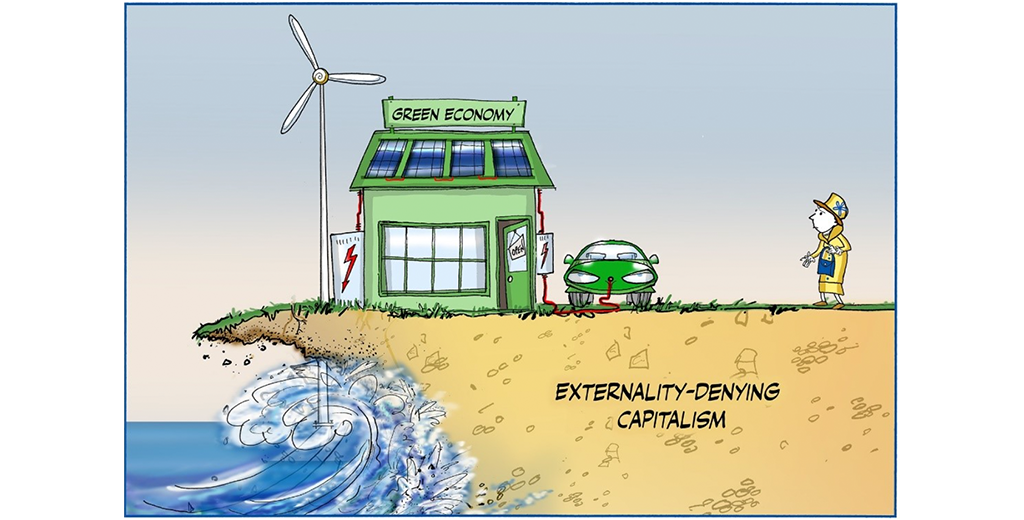
\includegraphics{fig/Market_Led _sustainability_is_a_fix_that_fails.png}

VML stands for two conflicting ideas at once. VML's explicit message is that we must urgently solve social and environmental problems. But the unavoidable, tacit meta-message of VML, as a market-based movement, is that `markets are the solution', which reinforces many of the underlying dynamics that perpetuate the problems.

A sustainability discourse conducted in business and economics terms continues to miss the physics for the finance. Our climate and biodiversity challenges are fundamentally driven by human transformation of matter and energy at a scale and pace that exceeds Nature's capacity to absorb. In response, VML aims to transform the world more sustainably, but the building of a clean economy has simply become the new banner by which we accelerate our transformation of the physical world. We frame the build-out of a clean economy as `greener', but the Earth just registers `yet more' transformation of matter and energy overwhelming natural processes. VML denies that a large part of our sustainability response requires establishing a slower and gentler interaction with Nature to fall back into balance with its pace. Less, not more.

Neoliberalism's capture of environmentalism is virtually complete.

\href{https://www.responsible-investor.com/articles/market-led-sustainability-is-a-fix-that-fails}{Austin (2021) Responsible Investor}

\href{https://bothbrainsrequired.com/2021/10/25/fix-that-fails/}{Austin (2021) Market-led Sustainability is a `Fix that Fails'\ldots\ldots but It May Have Been the Necessary `Defence at First Depth'}
\href{pdf/Austin_2021_Market_Led_Sustainability_Fix_Fails.pdf}{(pdf)}

\hypertarget{regulations}{%
\section{Regulations}\label{regulations}}

\hypertarget{carbon-pricing}{%
\section{Carbon Pricing}\label{carbon-pricing}}

\emph{Memo} See Volts

\hypertarget{part-appendices}{%
\part{Appendices}\label{part-appendices}}

\hypertarget{appendix-appendices}{%
\appendix}


\hypertarget{about}{%
\chapter{About}\label{about}}


\includegraphics{fig/me.jpg}

\emph{Dyre Haugen} and \emph{Dyrehaugen} is Webian for \emph{Jon Martin} -
self-owned Globian, Webian, Norwegian and Canarian with
a background from industrial research policy, urban planning and
economic development consulting on global, regional and urban scales.
I am deeply concerned about the (insane) way
humanity (i.e.~capitalism) interfere with nature.
In an effort to gain insights in how and why this happens
stuff is collected from around the web and put together
in a linked set of web-sites.
The sites are operated as personal notebooks.
However, these days things can be easily published to the
benefit of others concerned with the same issues.
But be aware - this is not polished for presentation or
peer-reviewed for exactness.
I offer you just to have a look at my `work-desk' as it appears in the moment.
Any comment or suggestion can be mailed to \href{mailto:dyrehaugen@gmail.com}{\nolinkurl{dyrehaugen@gmail.com}}
You can follow me on twitter as @dyrehaugen.
Thanks for visiting!

\hypertarget{links}{%
\chapter{Links}\label{links}}

\textbf{Current Dyrehaugen Sites:}

\begin{itemize}
\tightlist
\item
  \href{https://dyrehaugen.github.io/rcap}{rcap - On Capitalism} \href{http://localhost/rcap}{(loc)}
\item
  \href{https://dyrehaugen.github.io/rclm}{rclm - On Climate Change} \href{http://localhost/rclm}{(loc)}
\item
  \href{https://dyrehaugen.github.io/recs}{recs - On Economics} \href{http://localhost/recs}{(loc)}
\item
  \href{https://dyrehaugen.github.io/rngy}{rfin - On Finance} \href{http://localhost/rfin}{(loc)}
\item
  \href{https://dyrehaugen.github.io/rngy}{rngy - On Energy} \href{http://localhost/rngy}{(loc)}
\item
  \href{https://dyrehaugen.github.io/renv}{renv - On Environment} \href{http://localhost/renv}{(loc)}
\item
  \href{https://dyrehaugen.github.io/rsts}{rsts - On Statistics} \href{http://localhost/rsts}{(loc)}
\item
  \href{https://dyrehaugen.github.io/rurb}{rurb - On Urbanization} \href{http://localhost/rurb}{(loc)}
\item
  \href{https://dyrehaugen.github.io/rvar}{rvar - On Varia} \href{http://localhost/rvar}{(loc)}
\item
  \href{https://dyrehaugen.github.io/rwsd}{rwsd - On Wisdom} \href{http://localhost/rwsd}{(loc)}
\end{itemize}

\textbf{Blogs:}

\begin{itemize}
\tightlist
\item
  \href{https://dyrehaugen.github.io/rde}{rde - Blog in English} \href{http://localhost/rde}{(loc)}
\item
  \href{https://dyrehaugen.github.io/rdn}{rdn - Blog in Norwegian} \href{http://localhost/rdn}{(loc)}
\end{itemize}

\textbf{Discontinued:}

\begin{itemize}
\tightlist
\item
  \href{https://dyrehaugen.github.io/jdt}{jdt - Collection (Jekyll)} \href{http://localhost/jdt}{(loc)}
\item
  \href{https://dyrehaugen.github.io/hdt}{hdt - Collection (Hugo)} \href{http://localhost/hdt}{(loc)}
\end{itemize}

\textbf{Not listed:}

\begin{itemize}
\tightlist
\item
  (q:) dhe dhn jrw56
\item
  (z:) rcsa rpad rstart
\end{itemize}

\hypertarget{news}{%
\chapter{NEWS}\label{news}}

210704 TFND

An international Taskforce on Nature-related Financial Disclosures (TNFD) launched last month. Over the next two years, the TNFD will develop a framework for corporations and financial institutions to report on nature-related physical and transition risks that include immediate, material financial risks, as well as nature dependencies and impacts and related organisational and societal risks.

This ambitious scope of work has already been endorsed by the G7 finance ministers and, with the TNFD officially under way, nature risk will ascend quickly to claim its place alongside climate risk at the top of board agendas.

\href{https://www.theguardian.com/commentisfree/2021/jul/04/biodiversity-loss-could-wreck-the-global-financial-system-and-its-only-a-matter-of-time}{Guardian}

210703 Treaty to end Virgin Plastic Production

Since the 1950s about 8bn tonnes of plastic has been produced. The effects are everywhere. One of the reports authors, Nils Simon, said: ``Plastics are ubiquitously found in increasing amounts worldwide, including in terrestrial environments and even inside the human body.''

Science senior editor Jesse Smith, writes: ``As for much new technology, their development and proliferation occurred with little consideration for their impacts, but now it's impossible to deny their dark side as we confront a rapidly growing plastic pollution problem.

The report calls for a new global treaty ``to cover the entire lifecycle of plastics, from the extraction of the raw materials needed for its manufacture to its legacy pollution''.

The largest proportion of plastic waste comes from packaging materials (47\%), while textiles are responsible for 14\% and transport 6\%.

Each year, 3\% of worldwide plastic waste ends up in the oceans; in 2010 that amounted to about 8m tonnes of plastic.

Yet plastic production has continued to increase. In 2019, 368m tonnes of newly made, or virgin, plastics were produced. By 2050, the production of new plastic from fossil fuels could consume 10-13\% of the remaining global carbon budget permissible to ensure temperatures rise to no more than 1.5C above pre-industrial levels as required by the Paris climate agreement.

\href{https://www.theguardian.com/environment/2021/jul/01/call-for-global-treaty-to-end-production-of-virgin-plastic-by-2040}{The Guardian}

\emph{Simon}

Amid the global plastic pollution crisis, a growing number of governments and nongovernmental actors are proposing a new global treaty. In February 2021, at the fifth meeting of the United Nations Environment Assembly (UNEA)---the world's highest-level decision-making body on the environment---many governments spoke in favor of an international agreement to combat plastic pollution. In the past, the international community tended to view the plastics problem from a predominantly ocean-focused and waste-centered perspective. However, plastics are increasingly found in all environmental media, including terrestrial ecosystems and the atmosphere, as well as human matrices, including lungs and placenta. We therefore argue for a new international legally binding agreement that addresses the entire life cycle of plastics, from extraction of raw materials to legacy plastic pollution. Only by taking this approach can efforts match the magnitude and transboundary nature of this escalating problem and its social, environmental, and economic impacts. Targeting the full life cycle of plastics allows for a more equitable distribution of the costs and benefits of relevant actions across the global value chain.

\href{https://science.sciencemag.org/content/373/6550/43}{Simon (2021) A binding global agreement to address the life cycle of plastics (paywall)}

210623 Ecocide Defined

fter six months of deliberation, a team of international lawyers has unveiled a new legal definition of ``ecocide'' that, if adopted, would put environmental destruction on a par with war crimes -- paving the way for the prosecution of world leaders and corporate chiefs for the worst attacks on nature.

The expert panel published the core text of the proposed law on Tuesday, outlining ecocide as

\begin{quote}
``unlawful or wanton acts committed with knowledge that there is a substantial likelihood of severe and either widespread or long-term damage to the environment being caused by those acts''.
\end{quote}

Its authors want the members of the International Criminal Court (ICC) to endorse it and hold big polluters to account in a bid to halt the unbridled destruction of the world's ecosystems.

\href{https://www.aljazeera.com/news/2021/6/22/legal-experts-unveil-new-definition-ecocide}{Al Jazeera}

210411 Rare European vultures being poisoned by livestock drug

\textbf{Diclofenac}

A recently approved veterinary drug has been confirmed as the cause of death of a vulture in Spain. Conservationists say the incident could be the tip of an iceberg, and warn that the drug could wipe out many of Europe's vultures as well as harming related species, including golden eagles.

The anti-inflammatory agent diclofenac has already been banned in India, Pakistan, Nepal and Bangladesh after it was found to kill vultures that ate the carcasses of cattle treated with the drug. Tens of millions of vultures are believed to have died in this way with some species declining by a staggering 99.9\% in parts of south Asia.

Nevertheless diclofenac was approved in Spain and other European nations because farmers, drug companies and regulators argued that cattle carcasses were disposed of differently in Europe than in India. This meant vultures would not be able to eat meat tainted with diclofenac.

That claim has now been shown to be wrong.

Europe has four species of vulture: bearded, cinereous, Egyptian and griffon vultures. Recent research has also found that diclofenac not only kills vultures but is fatal to eagles of the genus Aquila whose members include the golden eagle and the Spanish imperial eagle. There are only about 300 pairs of imperial Spanish eagles left.

210406 Biodegradable Plastics from Fish Waste

Previous studies have developed methods for producing plastics from fish waste, but the latest research goes further in determining how the material might be easily broken down again at the end of its useful life.

To produce the new material, the researchers used oil extracted from bits of salmon left after the flesh had been removed and processed for human consumption.

They developed a way of converting the fish oil into a polyurethane-like polymer, first by adding oxygen to the oil in a controlled way to form epoxides, molecules similar to those in epoxy resin.

Then, carbon dioxide was added to the epoxides and the resulting molecules combined with nitrogen-containing chemical compound amines to form the new material.

``When we start the process with the fish oil, there is a faint kind of fish smell, but as we go through the steps, that smell disappears.''

Experiments suggested the new material might biodegrade readily when required.
In one, pieces of the plastic were soaked in water, some with lipase, an enzyme that breaks down fats in fish oil.
Under a microscope, the researchers saw microbial growth on the samples, including those that had been placed just in plain water. The team said the results offered an encouraging sign that the new material might biodegrade readily.

Polyurethanes are traditionally made using crude oil and phosgene, a toxic gas, and the process generates isocyanates, which are powerful irritants to the eyes and gastrointestinal and respiratory tracts, with links to severe asthma attacks.

In addition, the final product does not readily break down in the environment and the limited biodegradation that does occur can release carcinogenic compounds.

Past research has resulted in polyurethanes made using plant-derived oils to replace petroleum, however the researchers said these were not without their downsides either as the crops, often soybeans, require land and resources.

\href{https://www.independent.co.uk/news/science/plastic-fish-waste-biodegradable-study-b1826844.html}{Independent}

210322 Siberian Microplastics

Microplastics have been found in snow in Siberia, one of the world's remotest regions, in a sign of how far damaging human-made pollution has pervaded the environment.
Researchers gathered snow samples from 20 different Siberian regions - from the Altai mountains near Mongolia in the east to the Arctic, and said their preliminary findings confirmed that airborne plastic fibres were turning up in snow in these wildernesses.

``It's clear that it's not just rivers and seas that are involved circulating microplastics around the world, but also soil, living creatures and even the atmosphere,'' said Yulia Frank, scientific director at the university's Microplastics Siberia centre.

Tomsk scientists have previously found microplastics in the digestive systems of fish caught in Siberian rivers, confirming that the Arctic Ocean is polluted with microscopic plastics.

\href{https://www.independent.co.uk/climate-change/news/microplastic-snow-siberia-pollution-b1819682.html}{Independent}

\hypertarget{counting-elephants-from-space}{%
\section{210122 Counting Elephants from Space}\label{counting-elephants-from-space}}

Scientists have been able to identify Elephants from space for the first time - technology that could be used to empower efforts to challenge wildlife poaching.
Researchers used commercial earth observation satellites Worldview 3 and 4 to capture high resolution images of African elephants moving through grasslands and forests.
And combined with computer deep learning, an automated system was able to pick out animals with the same level of accuracy as a human would.

The algorithm, designed by Dr Olga Isupova of the University of Bath, could allow vast landmasses to be scanned and assessed in a matter of minutes - outpacing human observers who would typically carry out such work from low-flying planes.

Poaching as well as damage to habitats has caused the population of African elephants to nosedive in the past century, with roughly 415,000 savannah elephants believed to still be left in the wild.

\href{https://www.independent.co.uk/environment/wildlife-trade-campaign-study-elephants-b1790797.html}{Independent}

\hypertarget{biomass-energy-policy-got-it-wrong}{%
\section{210114 Biomass Energy Policy got it wrong}\label{biomass-energy-policy-got-it-wrong}}

`Green Energy' demand drives unsustainable logging, taking a toll on bird species
like the black grouse, woodlark and others. Woodland birds are declining.

The clearances are damaging the ability forests to store carbon,
undermine climate goals.

Wood pellets are sold as a clean alternative to coal. But is the subsidised bioenergy boom accelerating the climate crisis?

There is a direct connection between the subsidised growth in the biomass industry encouraged by EU renewable energy policies and the acceleration of unsustainable Baltic tree-felling

The intensification of logging is at least partly driven by higher demand for biomass for heat and power

A switch to burning wood in the form of pellets appears to offer a simple and in theory carbon-neutral alternative to coal-fired power stations because trees take up carbon dioxide from the air as they grow. As long as the burned trees are replaced with new plantings, there is no net addition to the stock of carbon in the atmosphere.

However, that process of carbon take-up can take many decades. And in the furnace, burning wood releases more carbon dioxide per unit of energy than burning gas, oil, or even coal. By accelerating carbon dioxide emissions in the short term, burning wood for electricity could be fatal for states' ability to meet the Paris Agreemen

A flaw in the legislation meant that woody biomass was fully categorised as renewable, even if it came not just from wood residues or waste, but from whole trees. This meant that companies could directly harvest forests for pellets -- rather than making pellets from the by-products of timber cut for other uses -- in the name of sustainable forest management.

As the EU moved in 2018 to double the use of renewable energy by 2030, scientists warned the European Parliament that this loophole in the sustainability criteria of the revised EU legislation would accelerate the climate crisis and devastate mature forests. But against the competing interests of the multibillion euro biomass lobby, it went unamended.

Scientists and campaigners say we simply don't have time to cut down trees for energy production if we are going to meet climate goals.

The urgency has completely changed in the last 15 years.
We don't have until 2070 -- emissions have to come down sooner.
Biomass that increases carbon emissions in the next 10 to 30 years
is not compatible with climate change policy.

\href{https://www.theguardian.com/world/2021/jan/14/carbon-neutrality-is-a-fairy-tale-how-the-race-for-renewables-is-burning-europes-forests}{Guardian}

\hypertarget{rewilding-farming}{%
\subparagraph{210102 Rewilding Farming}\label{rewilding-farming}}

\begin{quote}
In West Sussex, England, Charlie Burrell and Isabella Tree have let their property become overrun
and the rsults are spectacular.
The 3,500 acre-Knepp Estate was once a traditional farm, but poor agricultural land and
a ``pretty bleak'' financial future forced a change of direction from the couple.
Over the last 20 years they have let their livestock roam free, and nature has flooded
back in alongside the pigs and deer.
Species that were never previously seen in the area, like the turtle dove and
the purple emperor butterfly, have set up in Knepp and thrived.
``To see the landscape of your own country, and what you've been missing, suddenly come to life has been this extraordinary revelation,'' says Burrell.
\end{quote}

\href{https://edition.cnn.com/2020/10/01/world/knepp-farm-rewilding-scn-cte-spc/index.html}{Rewilding (CNN)}

\hypertarget{biological-conservation}{%
\section{201231 Biological Conservation}\label{biological-conservation}}

Horizon scanning is a form of foresight research.
For 12 years it has been practized for identification of upcoming
biological conservation issues.
The 2021 scanning presents these major issues

\begin{itemize}
\item
  Underestimated Effects of Deoxygenation on Coral Reef Health and Survival
\item
  Increases in Dissolved Iron Availability and Polar Coastal Productivity
\item
  Substantial Increase in Decommissioning of Offshore Energy Platforms
\item
  Use of Seabirds to Locate Fishing Vessels Remotely
\item
  Proliferation of False Information Reported by Global Navigation Satellite and Automatic
  Identification Systems
\item
  Multigenerational Effects of Low Levels of Exposure to Endocrine Disruptors
\item
  Changes in Coastal Low Clouds
\item
  Challenges to Tree Plantations as a Simple Carbon Sequestration Solution
\item
  Increased Logging in Response to Fire Risk
\item
  Complete Coverage of Indian States with Sustainable Farming
\item
  Low Earth Orbit Satellites May Mislead Animals Responding to Celestial Cues
\item
  Emergence of a Global Market for Stranded Energy
\item
  Open-Source Investigation of Environmental Threats
\item
  Self-Healing Building Materials
\item
  2000-km E40 Waterway Linking the Baltic and Black Seas
\end{itemize}

\href{https://www.theguardian.com/environment/2020/dec/28/seabird-patrols-to-self-healing-buildings-the-15-conservation-stories-to-watch-in-2021}{Biological Conservation Issues (The Guardian)}

\href{https://www.cell.com/trends/ecology-evolution/fulltext/S0169-5347(20)30306-2}{Emerging Global Biological Conservation Issues (article)}
\href{/pdf/Sutherland_2020_Horizon_Scan_Biological_Conservation_Issues.pdf}{(pdf)}

\hypertarget{architecture-of-degrowth}{%
\section{201231 Architecture of Degrowth}\label{architecture-of-degrowth}}

\href{http://oslotriennale.no/en/aboutoat2019}{ENOUGH Oslo Architecture Trienale}
\textgreater For the last two centuries, the engine of architectural production and the basis of societies around the world has been the pursuit of economic growth. The desire for infinite growth has forced aside common and ecological goals measuring acts of culture and community as mere bumps in GDP. Yet the limits to this paradigm have become abundantly clear. As equity, wellbeing and non-monetary measures of prosperity falter, rising sea temperatures, extreme weather and other indicators of climate breakdown converge on the conclusion that the days of growth's predominance are running out.

\begin{quote}
Architecture is no exception. The promise of a meaningful life's work harnessing the transformative power of design to mix beauty and social justice is deeply felt. Yet for many, our daily practice looks very different to the work we aspired to. The majority of urban practitioners are not the agents of social change they might have been, but cogs in a vast value-producing machine whose hunger for expansion is never abated. Homes have become vehicles of capital speculation, galleries have become billboards for attracting investment, streets have become the infrastructure of consumption, universities export enlightenment for profit.
\end{quote}

\begin{quote}
In our bones we know that infinite economic growth is impossible. We know that money cannot buy happiness. We know that change is coming. Yet our professions continue to toil at the coalface of economic expansion cultivating consumption in pursuit of a prize that is never enough.
\end{quote}

\begin{quote}
ENOUGH responds to an era of climate emergency and social inequality by proposing alternatives to the unsustainable and unfair paradigm of growth. The festival explores the architecture of Degrowth, an economy of shared plenty in which human and ecological flourishing matter most. It is time to call time on too much for the few and too little for the many. Join us as we propose a vision of Enough for all.
\end{quote}

\href{https://failedarchitecture.com/degrowth-is-about-redistribution-by-design-not-by-collapse/}{Failed Archtecture}

\hypertarget{royal-insanity}{%
\section{201230 Royal Insanity}\label{royal-insanity}}

\href{https://www.independent.co.uk/life-style/royal-family/prince-charles-radio-4-indigenous-communities-b1779998.html}{The Independent}
The Prince of Wales has described humanity's exploitation of nature as ``insanity''.
Speaking to novelist Margaret Atwood on BBC Radio 4's Today Programme, Prince Charles explained how humans have become increasingly detached from the natural world in recent years.
``We are a microcosm of the macrocosm, but we've forgotten that, or somehow been brainwashed into thinking that we have nothing to do with nature, nature can just be exploited,'' he said.
``And if we go on exploiting where we are, whatever we do to nature, however much pollution, we do to ourselves - it is insanity.''
Charles also urged people to listen to the ``wisdom of indigenous communities'' in order to better understand how to combat the climate crisis.

May be time to get back to Enlightened Monarchy

  \bibliography{book.bib,packages.bib}

\end{document}
